\documentclass[11pt,a4paper]{article}

\usepackage[utf8]{inputenc}
\PassOptionsToPackage{hyphens}{url}
\usepackage{amsmath,amssymb,amsthm}
\usepackage{mathtools}
\usepackage{graphicx}
\usepackage{booktabs}
\usepackage{array}
\usepackage[hypertexnames=false,colorlinks=true,linkcolor=blue,citecolor=blue,urlcolor=blue,pdfauthor={Kyle Elliott Mathewson},pdftitle={Mechanics and Balance of Magic Gems: Radial Vector Laws, Symmetric-Top Precession, Nested Core Inclusions, and Mirror-Twin Towers}]{hyperref}
\usepackage{geometry}
\usepackage{float}

% \Cref / \cref: reference with the type name inferred from the label prefix (fig:, thm:, sec:, ...).
\makeatletter
\def\Cref@getprefix#1:#2\relax{#1}
\def\Cref@prefix@sec{sec}
\def\Cref@prefix@subsec{subsec}
\def\Cref@prefix@fig{fig}
\def\Cref@prefix@tab{tab}
\def\Cref@prefix@eq{eq}
\def\Cref@prefix@thm{thm}
\def\Cref@prefix@prop{prop}
\def\Cref@prefix@lem{lem}
\def\Cref@prefix@cor{cor}
\def\Cref@prefix@conj{conj}
\def\Cref@prefix@def{def}
\def\Cref@prefix@rem{rem}
\def\Cref@prefix@ex{ex}

\def\Cref@type@cap#1{%
  \edef\Cref@tmp{#1}%
  \ifx\Cref@tmp\Cref@prefix@sec Section%
  \else\ifx\Cref@tmp\Cref@prefix@subsec Section%
  \else\ifx\Cref@tmp\Cref@prefix@fig Figure%
  \else\ifx\Cref@tmp\Cref@prefix@tab Table%
  \else\ifx\Cref@tmp\Cref@prefix@eq Equation%
  \else\ifx\Cref@tmp\Cref@prefix@thm Theorem%
  \else\ifx\Cref@tmp\Cref@prefix@prop Proposition%
  \else\ifx\Cref@tmp\Cref@prefix@lem Lemma%
  \else\ifx\Cref@tmp\Cref@prefix@cor Corollary%
  \else\ifx\Cref@tmp\Cref@prefix@conj Conjecture%
  \else\ifx\Cref@tmp\Cref@prefix@def Definition%
  \else\ifx\Cref@tmp\Cref@prefix@rem Remark%
  \else\ifx\Cref@tmp\Cref@prefix@ex Example%
  \else Ref.%
  \fi\fi\fi\fi\fi\fi\fi\fi\fi\fi\fi\fi\fi
}

\def\Cref@type@low#1{%
  \edef\Cref@tmp{#1}%
  \ifx\Cref@tmp\Cref@prefix@sec section%
  \else\ifx\Cref@tmp\Cref@prefix@subsec section%
  \else\ifx\Cref@tmp\Cref@prefix@fig figure%
  \else\ifx\Cref@tmp\Cref@prefix@tab table%
  \else\ifx\Cref@tmp\Cref@prefix@eq equation%
  \else\ifx\Cref@tmp\Cref@prefix@thm theorem%
  \else\ifx\Cref@tmp\Cref@prefix@prop proposition%
  \else\ifx\Cref@tmp\Cref@prefix@lem lemma%
  \else\ifx\Cref@tmp\Cref@prefix@cor corollary%
  \else\ifx\Cref@tmp\Cref@prefix@conj conjecture%
  \else\ifx\Cref@tmp\Cref@prefix@def definition%
  \else\ifx\Cref@tmp\Cref@prefix@rem remark%
  \else\ifx\Cref@tmp\Cref@prefix@ex example%
  \else ref.%
  \fi\fi\fi\fi\fi\fi\fi\fi\fi\fi\fi\fi\fi
}

\DeclareRobustCommand{\Cref}[1]{%
  \begingroup
  \edef\Cref@label{#1}%
  \edef\Cref@prefix{\expandafter\Cref@getprefix\Cref@label:\relax}%
  \hyperref[#1]{\Cref@type@cap{\Cref@prefix}~\ref*{#1}}%
  \endgroup
}
\DeclareRobustCommand{\cref}[1]{%
  \begingroup
  \edef\Cref@label{#1}%
  \edef\Cref@prefix{\expandafter\Cref@getprefix\Cref@label:\relax}%
  \hyperref[#1]{\Cref@type@low{\Cref@prefix}~\ref*{#1}}%
  \endgroup
}
\makeatother

\geometry{margin=0.9in}
\setlength{\emergencystretch}{2em}
\setlength{\textfloatsep}{10pt plus 2pt minus 2pt}
\setlength{\intextsep}{8pt plus 2pt minus 2pt}
\setlength{\abovecaptionskip}{4pt}
\makeatletter
\long\def\@makecaption#1#2{\vskip\abovecaptionskip\small\sbox\@tempboxa{#1: #2}\ifdim\wd\@tempboxa>\hsize #1: #2\par\else\global\@minipagefalse\hb@xt@\hsize{\hfil\box\@tempboxa\hfil}\fi\vskip\belowcaptionskip}
\makeatother
\renewcommand{\topfraction}{0.9}
\renewcommand{\bottomfraction}{0.6}
\renewcommand{\textfraction}{0.07}
\renewcommand{\floatpagefraction}{0.85}
\setcounter{topnumber}{3}
\setcounter{totalnumber}{5}

% Theorem environments
\theoremstyle{plain}
\newtheorem{theorem}{Theorem}[section]
\newtheorem{lemma}[theorem]{Lemma}
\newtheorem{proposition}[theorem]{Proposition}
\newtheorem{corollary}[theorem]{Corollary}
\newtheorem{conjecture}[theorem]{Conjecture}

\theoremstyle{definition}
\newtheorem{definition}[theorem]{Definition}
\newtheorem{example}[theorem]{Example}

\theoremstyle{remark}
\newtheorem{remark}[theorem]{Remark}

% Custom commands
\newcommand{\R}{\mathbb{R}}
\newcommand{\Z}{\mathbb{Z}}
\newcommand{\N}{\mathbb{N}}
\newcommand{\Q}{\mathbb{Q}}
\newcommand{\tr}{\operatorname{tr}}
\newcommand{\conv}{\operatorname{conv}}
\newcommand{\vertset}{\operatorname{vert}}
\newcommand{\vol}{\operatorname{vol}}
\newcommand{\cone}{\operatorname{cone}}
\newcommand{\diag}{\operatorname{diag}}

\title{\textbf{Mechanics and Balance of Magic Gems:\\ Radial Vector Laws, Symmetric-Top Precession,\\ Nested Core Inclusions, and Mirror-Twin Towers}}

\author{Kyle Elliott Mathewson\\
\textit{Faculty of Science, University of Alberta}\\
\texttt{kyle.mathewson@ualberta.ca}}

\date{}

\begin{document}

\maketitle

\begin{abstract}
A magic square is a combinatorial paradigm of \emph{balance in inequality}: its $n^2$ entries $\{1,\dots,n^2\}$ are strictly distinct, yet every row, column, and main diagonal sums to the same constant $\mu_n=n(n^2+1)/2$. Lifting the centred grid cells into $\R^3$ as radial vectors $\mathbf p_{ij}(\lambda)=(x_j,y_i,\lambda z_{ij})$ and taking their convex hull—the \emph{Magic Gem} $\mathcal G_\lambda(S)$—raises a central mechanical question: when does combinatorial line-sum equality suffice for physical equilibrium in three dimensions, and when a nonlinear physical realization breaks that balance, how can an opposing inequality restore it? We test this principle across all $880$ order-four magic squares by progressing from one-dimensional radial spokes to three-dimensional rotation, continuous solid and skeletal hulls, and freestanding stacked columns. For radial spokes from the origin $O$, natural vector lengths balance identically, whereas trimming the spokes to equal unit length breaks equilibrium on all $832$ non-associative squares in 3D and on every square in 2D, where the irrational ring-radius ratio $r_2/r_1=\sqrt{5}$ bounds the resultant below by the Pell convergent $9/4\approx\sqrt{5}$ ($18\sqrt{10}/5-8\sqrt{2}\approx0.0705$). By length--weight duality, radial equilibrium is restored either by assigning positive unequal tip weights $\mathbf w^*>\mathbf 0$ on the unit sphere $S^2$ or by scaling spoke lengths as a power law ($r^{\alpha^*}$ in 2D and cubic vertical vanishing $(\mathbf V_3)_z=0$ in 3D). In three-dimensional rotation, equal point masses at the unequal vertices $\mathbf p_{ij}(\lambda)$ make every semi-magic square an axisymmetric top with universal inertia ratio $I_\perp(\lambda)/I_{zz}=\frac12(1+\lambda^2(n^2+1))$ and spherical-top transition $\lambda_{\mathrm{iso}}=(n^2+1)^{-1/2}$, whereas weighting the vertices by their unequal entries $m_{ij}=s_{ij}$ exposes the quadrant quadrupole $Q_{xy}=\sum z_{ij}x_jy_i$, splitting the horizontal principal moments by $2|Q_{xy}|$ and triggering $180^\circ$ Dzhanibekov flips on $824$ squares. Passing from discrete points to the uniform solid hull $\mathcal G_0(S)$ shifts the centre of mass off $O$ on $829$ squares because interior grid points $P_S^{(1)}$ are omitted and hull facets are weighted by unequal simplex volumes; because the outer hull vertices and inner core points pull in strictly opposite directions ($V_0\overline{\mathbf p}_{\mathrm{outer}}+V_1\overline{\mathbf p}_{\mathrm{inner}}=\mathbf 0$), re-engaging the inner core $\mathcal G_1(S)=\conv P_S^{(1)}$ restores balance via two-density core inclusions, two-gauge nested wireframes, or the complete $\binom{n^2}{2}$-rod network $K_{n^2}$ ($\Sigma_{\mathrm{rods}}=\frac{2n^2-3}{3(n^2-1)}\Sigma(\lambda)$), while every boundary hull unfolds into a non-overlapping papercraft net with $f_0-1$ glue tabs. Finally, compressing the vertical aspect to the cubic print scale $\lambda=1/5$ stabilizes $74.5\%$ of all gem facets on a flat table, and alternating any gem $\mathcal G_\lambda(S)$ with its inverted mirror twin $\mathcal G_\lambda(r^2\overline S)=-\mathcal G_\lambda(S)$ cancels opposing facet tilts to lock chiral blocks into a straight vertical tower.
\end{abstract}

\section{Introduction}
\label{sec:intro}

Over five centuries ago, Albrecht D\"urer contributed two enduring landmarks at the intersection of mathematics and the visual arts: the order-four magic square in his 1514 engraving \emph{Melencolia~I} (square \#175 in Fr\'enicle's 1693 census of the $880$ order-four magic squares \cite{frenicle1693,dudeney1917amusements,andrews1960magic}) and the first printed polyhedral net unfoldings in his 1525 treatise \emph{Underweysung der Messung} \cite{durer1525underweysung,shephard1975convex,demaine2007geometric,ghomi2014durer}. Recall that an arrangement $S=(s_{ij})_{0\le i,j<n}$ of the integers $\{1,\dots,N\}$, $N=n^2$, is a \emph{semi-magic square} if every row and column sums to the magic constant $\mu_n=n(N+1)/2$, and a \emph{magic square} if the two main diagonals also sum to $\mu_n$. Measuring coordinates from the board centre and the mean entry $\bar s=(N+1)/2$,
\begin{equation}
\label{eq:coords}
x_j = j - \frac{n-1}{2},\qquad
y_i = \frac{n-1}{2} - i,\qquad
z_{ij} = s_{ij} - \frac{N+1}{2},
\end{equation}
turns each cell $(i,j)$ into a three-dimensional point and radial vector from the origin $O=(0,0,0)$:
\[
\mathbf p_{ij}(\lambda) = (x_j,\, y_i,\, \lambda z_{ij}) \in \R^3,\qquad
P_S(\lambda) = \bigl\{\mathbf p_{ij}(\lambda) : 0\le i,j<n\bigr\},
\]
where $\lambda>0$ is the vertical lift scale (\Cref{fig:origin-vectors-3d}(a)). The convex hull
\[
\mathcal G_\lambda(S) := \conv P_S(\lambda) \subset \R^3
\qquad\bigl(\mathcal G(S):=\mathcal G_1(S)\bigr)
\]
is a three-dimensional convex polyhedron that we call the \emph{Magic Gem} of $S$, reuniting D\"urer's magic squares with his polyhedral geometry.

In classical work on the planar mechanics of magic squares, Loly \cite{loly2004invariance} and Rogers and Loly \cite{rogers2004inertia,rogers2005multipole} interpreted the entries $s_{ij}$ as point masses on the flat grid $\mathbf r_{ij}=(x_j,y_i)$, proving that the planar centre of mass lies at the origin $O$ and that the polar moment of inertia $\sum_{i,j}s_{ij}(x_j^2+y_i^2)=n^2(n^4-1)/12$ is invariant across all semi-magic squares of order $n$. Inspired by fabricating physical 3D-printed models, radial balance wheels, ball-and-rod wireframes, interconnected strut sculptures, and folded cardstock cutouts in the open-source \texttt{magicGemWeb} studio \cite{mathewson2025magicgemweb}, this paper investigates one unifying physical and sculptural question across dimensions:

\begin{quote}
\itshape
When a magic square is lifted into $\R^3$ and fabricated as a physical sculpture---whether as a $16$-spoke radial star or weighted balance wheel from the origin (\Cref{sec:vectors}), a kinetic spinning top on a central pivot (\Cref{sec:dynamics}), a cast solid, nested two-material core, 3D-printed wireframe, complete $K_{16}$ strut network, or folded papercraft shell (\Cref{sec:nested}), or a freestanding column of stacked blocks (\Cref{sec:stacking})---when does the combinatorial balance of the magic square translate into physical equilibrium, smooth rotation, and structural stability?
\end{quote}

\Cref{fig:hero-squares} introduces the six flagship order-four magic squares (\#175, \#70, \#45$\leftrightarrow$\#54, \#46, \#673, and \#763$\leftrightarrow$\#756) that serve as our recurring physical exemplars across four progressive mechanical regimes:

\begin{figure}[htbp]
\centering
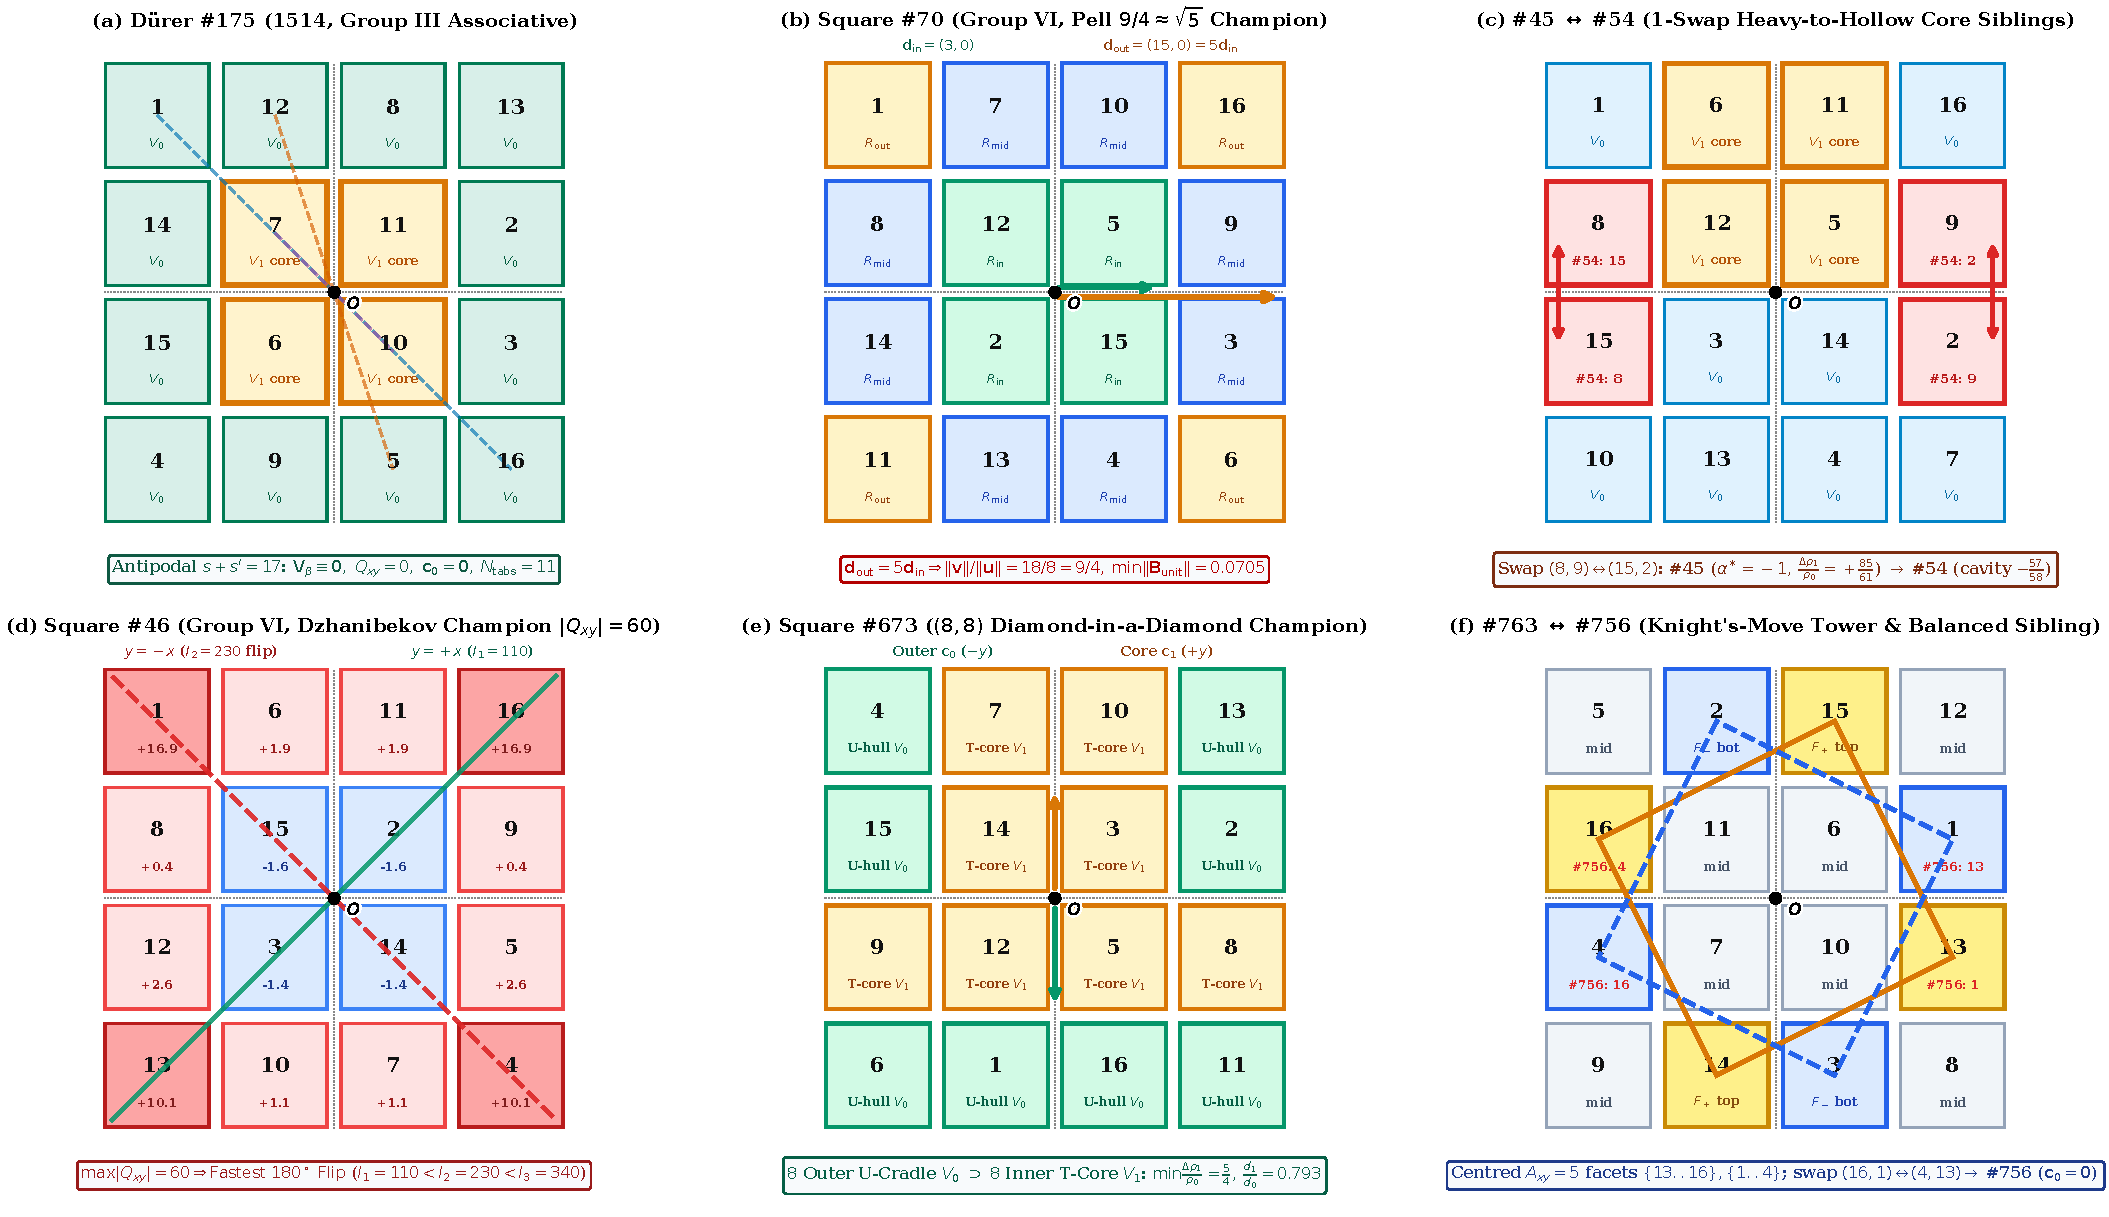
\includegraphics[width=\textwidth]{figures/fig_hero_squares_gallery.pdf}
\caption{Visual anatomy of the six flagship order-four magic squares across Sections~\ref{sec:vectors}--\ref{sec:stacking}. (a)~D\"urer's associative square \#175 (1514, Group~III), whose antipodal pairs sum to $17$ across $O$, partitioning into $12$ outer hull vertices $V_0$ and $4$ inner core vertices $V_1=\{6,7,10,11\}$. (b)~Square \#70 (Group~VI), coloured by concentric rings $R_{\mathrm{in}},R_{\mathrm{mid}},R_{\mathrm{out}}$, where parallel ring dipoles $\mathbf d_{\mathrm{out}}=(15,0)=5\mathbf d_{\mathrm{in}}$ achieve the fundamental Pell ratio $\|\mathbf v\|/\|\mathbf u\|=18/8=9/4\approx\sqrt{5}$. (c)~Square \#45 ($\kappa=+9$, inverse-radial root $\alpha^*=-1$, heavy core $\Delta\rho_1/\rho_0=+85/61$), where swapping the single outer border pair $(8,9)\leftrightarrow(15,2)$ between rows~$2$ and~$3$ yields sibling \#54 with the same $(V_0,V_1)=(10,6)$ vertex partition but a nearly hollow core cavity ($\Delta\rho_1/\rho_0=-57/58$). (d)~Square \#46 (Group~VI), shaded by cell quadrupole contribution $z_{ij}x_jy_i$, attaining the global maximum $|Q_{xy}|=60$ ($I_1=110<I_2=230<I_3=340$) and fastest $180^\circ$ Dzhanibekov flip about $y=-x$. (e)~Square \#673 (Group~VI), whose $8$ outer vertices form a U-cradle $V_0$ enclosing an $8$-vertex inverted-T core $V_1$, achieving the minimum solid excess density $\Delta\rho_1/\rho_0=5/4$. (f)~Square \#763 (Group~VI), whose centred $2\times1$ knight's-move facets $\{13,14,15,16\}$ and $\{1,2,3,4\}$ lock into an area-$5$ mirror-twin tower, and whose single border-pair swap $(16,1)\leftrightarrow(4,13)$ produces the naturally balanced solid \#756 ($\mathbf c_0=\mathbf 0$).}
\label{fig:hero-squares}
\end{figure}

\begin{enumerate}
\item \textbf{Radial spoke sculptures and balance wheels from the origin (\Cref{sec:vectors}).} Scaling 3D spoke lengths by $L_{ij}=R_{ij}(\lambda)^\beta$ is mechanically dual to weighting natural vectors $\mathbf p_{ij}(\lambda)$ by $w_{ij}=R_{ij}(\lambda)^{\beta-1}$ (\Cref{prop:reciprocity}). In 3D (\Cref{thm:3d-power}, \Cref{fig:origin-vectors-3d}), cubic spokes ($\beta=3$) have a strictly vanishing vertical resultant $(\mathbf V_3)_z=0$ for every semi-magic square, while on the unit sphere $S^2$ ($\beta=0$) every order-four square admits strictly positive minimum-variance weights $\mathbf w^*(S)>\mathbf 0$ restoring $\sum w_{ij}^*\hat{\mathbf p}_{ij}=\mathbf 0$. In the grid plane (\Cref{thm:three-ring}, \Cref{fig:ring-vectors}), decomposing $A_4$ into three concentric rings of radii $r_1=\sqrt{2}/2$, $r_2=\sqrt{10}/2$, and $r_3=3\sqrt{2}/2$ proves that unit-length planar spokes ($\alpha=0$) can never balance because $r_2/r_1=\sqrt{5}\notin\Q$; instead, $\min_{\mathcal M_4}\|\mathbf B_{\mathrm{unit}}(S)\|_2=\frac{18\sqrt{10}}{5}-8\sqrt{2}\approx0.0705$ is governed by the Pell convergent $9/4\approx\sqrt{5}$ on eight Group~VI squares led by \#70 (\Cref{fig:hero-squares}(b)), while $204$ squares with parallel dipoles $\mathbf d_{\mathrm{out}}=\kappa\mathbf d_{\mathrm{in}}$ admit a second power-law root $\alpha^*(\kappa)\ne1$, including $25$ at $\alpha^*=-1$ (\#45, \Cref{fig:hero-squares}(c)) and $25$ at $\alpha^*=+3$ (\#286; \Cref{cor:planar-power-roots}).

\item \textbf{Three-dimensional rotation: symmetric-top precession and Dzhanibekov flips (\Cref{sec:dynamics}).} For equal point masses at $\mathbf p_{ij}(\lambda)$, vanishing of the first moments makes the inertia tensor about $O$ strictly axisymmetric with universal ratio $I_\perp(\lambda)/I_{zz}=\frac12(1+\lambda^2(n^2+1))$ (\Cref{thm:rotor}, \Cref{fig:precession}(a)): every point-weighted gem passes through an exact \emph{spherical-top transition} at $\lambda_{\mathrm{iso}}=(n^2+1)^{-1/2}$ ($1/\sqrt{17}\approx0.2425$ at $n=4$) and a $9:1$ closed-orbit prolate regime at $\lambda=1$. Conversely, entry-weighted masses $m_{ij}=s_{ij}$ (\Cref{thm:quadrupole-split}) split the horizontal principal moments by $2|Q_{xy}(S)|=2|\sum z_{ij}x_jy_i|$ along $y=\pm x$ and couple the vertical products of inertia to $\mathbf V_3(S;\lambda)$, triggering $180^\circ$ Dzhanibekov flips on $824$ of the $880$ squares (led by \#46 at $|Q_{xy}|=60$, \Cref{fig:hero-squares}(d) and \Cref{fig:precession}(b--d)).

\item \textbf{Restoring solid, skeletal, and thin-shell balance via ``diamond-in-a-diamond'' layers, complete $K_N$ networks, and papercraft nets (\Cref{sec:nested}).} Casting a uniform solid $\mathcal G_0(S)=\conv P_S$ shifts $\mathbf c_0(S)$ away from $O$ on $829$ of the $880$ squares, leaving $51$ naturally balanced solids ($48$ associative plus Group~VI squares \#86, \#739, and \#756; \Cref{prop:51-balanced}). Peeling $\mathcal G_0(S)\supset\mathcal G_1(S)$ (\Cref{prop:opposition}) yields $35$ two-density balanced solids (\Cref{thm:diamond-balance}, \Cref{fig:nested-diamonds}): $33$ with a denser inner core (led by \#673 at $\Delta\rho_1/\rho_0=5/4$, \Cref{fig:hero-squares}(e)) and $2$ (\#123 and \#54, \Cref{fig:hero-squares}(c)) where volumetric simplex weighting pulls $\mathbf c_0$ to the same side of $O$ as $\mathbf c_1$, requiring a lighter or nearly hollow core cavity. For skeletal and sheet fabrications (\Cref{subsec:wireframes-nets}, \Cref{fig:wireframes-nets}), the complete $\binom{N}{2}$-rod network $K_N$ with equal-mass rods has $\mathbf c(K_N)=\mathbf 0$ and $\Sigma_{\mathrm{rods}}=\frac{2N-3}{3(N-1)}\Sigma(\lambda)=\frac{29}{45}\Sigma(\lambda)$ at $n=4$ (\Cref{thm:complete-network}), tuning inner-to-outer rod diameters $d_1/d_0$ balances $158$ Group~VI wireframes at $\lambda=1$ ($164$ at $\lambda=0.20$), and every gem unfolds along a breadth-first dual spanning tree into a non-overlapping 2D papercraft net with $N_{\mathrm{tabs}}=f_0-1$ glue tabs (\Cref{prop:papercraft-net}).

\item \textbf{Mirror-twin facet locking and chiral vertical towers (\Cref{sec:stacking}).} While only $124$ of the $880$ gems have parallel top and bottom facets on the \emph{same} gem, the half-turned complement $S^*=r^2\overline S$ satisfies $\mathcal G_\lambda(S^*)=-\mathcal G_\lambda(S)$ (\Cref{thm:mirror-tower}), pairing every upper facet $F_+\subset\mathcal G_\lambda(S)$ with a congruent parallel lower facet $-F_+\subset\mathcal G_\lambda(S^*)$. Alternating unrotated translates of $\mathcal G_\lambda(S)$ and $\mathcal G_\lambda(S^*)$ along centrally symmetric vertical-axis facets forms a zero-drift vertical tower for $48$ gems (\Cref{prop:knights-move}, \Cref{fig:mirror-stacking}), led by $17$ gems with area-$5$ centred knight's-move square facets such as chiral Group~VI gem \#763 (\Cref{fig:hero-squares}(f), \Cref{rem:chirality}).
\end{enumerate}

Every theorem and census table in this paper is certified in exact integer and rational arithmetic (\texttt{fractions.Fraction}) by \texttt{anc/verify\_paper\_c.py} (\Cref{sec:appendix}), and all five mechanical regimes can be explored in real time in the companion interactive browser visual essay (\texttt{web/index.html}).

\paragraph{Conventions, indexing, and relation to companion work.}
Let $A_n=\{(x_j,y_i):0\le i,j<n\}$ denote the centred grid \eqref{eq:coords}, let $a_n=(n^2-1)/12$ and $b_n=(n^4-1)/12=(n^2+1)a_n$ denote the marginal variances of $x_j$ and $z_{ij}$, and let the dihedral group $D_4=\langle r,h\rangle$ (with $90^\circ$ rotation $r$ and horizontal/vertical reflections $h,v$) act on arrangements together with the complement involution $\tau(S)=\overline S=(N+1)\mathbf 1-S$. An arrangement $S$ is \emph{associative} (Dudeney's Group~III of $48$ squares at $n=4$, including D\"urer's \#175) if $r^2 S=\overline S$, i.e.\ $z(-x,-y)=-z(x,y)$, and belongs to Dudeney's \emph{Group~VI} ($304$ squares at $n=4$) if $\overline S$ equals $hS$ or $vS$, inducing a $180^\circ$ half-turn symmetry ($C_2\subset SO(3)$) of $\mathcal G_\lambda(S)$ in $\R^3$. Companion preprints \cite{mathewson2026gems,mathewson2026moments} catalogue the static polyhedral combinatorics and bivariate Prouhet--Tarry--Escott moment hierarchy of semi-magic squares; the present paper is self-contained. Order-four magic squares are numbered $\#1,\dots,\#880$ by their 1-based position in Fr\'enicle's standard list (\texttt{anc/squares880.txt}); Tables~\ref{tab:two-density} and \ref{tab:knights-move} also list the 0-based index ($\#0=\#1-1$).

\section{Test 1: Radial Spokes from the Origin and Length--Weight Duality}
\label{sec:vectors}

In the fabrication suite \texttt{magicGemWeb} \cite{mathewson2025magicgemweb}, the $16$ cells of an order-four magic square are built as two radial sculptures pivoted at the origin $O$: (i)~a \emph{3D $16$-spoke hub-and-strut star} (\texttt{magicGem.scad}, \Cref{fig:origin-vectors-3d}(a)) with spokes $\mathbf p_{ij}(\lambda)=(x_j,y_i,\lambda z_{ij})$ of length $R_{ij}(\lambda)=\|\mathbf p_{ij}(\lambda)\|_2$ along unit directions $\hat{\mathbf p}_{ij}(\lambda)=\mathbf p_{ij}(\lambda)/R_{ij}(\lambda)\in S^2$; and (ii)~a \emph{planar $16$-spoke balance wheel} on a conical fulcrum (\texttt{weighted\_ring.stl}, \Cref{fig:ring-vectors}(a)) with spokes along $\mathbf r_{ij}=(x_j,y_i)$ of radius $r_{ij}=\|\mathbf r_{ij}\|_2$ and unit direction $\mathbf u_{ij}=\mathbf r_{ij}/r_{ij}\in S^1$. At natural linear lengths ($L_{ij}=R_{ij}(\lambda)$ or $\ell(r_{ij})=r_{ij}$), both sculptures balance identically at $O$ because $\sum_{i,j}\mathbf p_{ij}(\lambda)=\mathbf 0$ and $\sum_{i,j}z_{ij}\mathbf r_{ij}=\mathbf 0$ \cite{loly2004invariance,rogers2005multipole}, closing the $16$ planar vectors into a head-to-tail polygon (\Cref{fig:ring-vectors}(b)).

Our first test probes the mechanism of this equilibrium: \emph{does radial balance reside in the directions of the spokes alone, or does it rely on the unequal spoke lengths compensating the unequal directions? When equalizing spoke lengths breaks balance, how can an opposing inequality in tip weights or power-law lengths restore it?}

\subsection{Length--Weight Duality: Why Equalizing Spoke Lengths Breaks Balance}

\begin{definition}[Generalized 3D and planar origin-vector resultants]
\label{def:radial-resultant}
For an arrangement $S$ of order $n$ and vertical lift scale $\lambda>0$, let $R_{ij}(\lambda)=\sqrt{x_j^2+y_i^2+\lambda^2z_{ij}^2}$ and $\hat{\mathbf p}_{ij}(\lambda)=\mathbf p_{ij}(\lambda)/R_{ij}(\lambda)$ ($\mathbf 0$ if $R_{ij}(\lambda)=0$). Given cell weights $w=(w_{ij})$ and prescribed 3D spoke lengths $L=(L_{ij})$, the \emph{3D origin-vector resultant} is
\begin{equation}
\label{eq:V-3d-general}
\mathbf V_{w,L}(S;\lambda) = \sum_{i,j} w_{ij}\,L_{ij}\,\hat{\mathbf p}_{ij}(\lambda)
= \sum_{R_{ij}(\lambda)>0} \left(\frac{w_{ij}L_{ij}}{R_{ij}(\lambda)}\right)\mathbf p_{ij}(\lambda) \in \R^3.
\end{equation}
For equal weights $w_{ij}=1$ and power-law 3D lengths $L_{ij}=R_{ij}(\lambda)^\beta$ ($\beta\in\R$), we write
\begin{equation}
\label{eq:V-beta}
\mathbf V_\beta(S;\lambda) := \sum_{i,j} R_{ij}(\lambda)^\beta\,\hat{\mathbf p}_{ij}(\lambda)
= \sum_{i,j} R_{ij}(\lambda)^{\beta-1}\,\mathbf p_{ij}(\lambda) \in \R^3,
\end{equation}
and for weighted unit vectors ($L_{ij}=1$) on $S^2$, we write $\mathbf B^{(3)}_{w,\lambda}(S):=\mathbf V_{w,1}(S;\lambda)=\sum_{i,j}w_{ij}\hat{\mathbf p}_{ij}(\lambda)$. Similarly, in the grid plane, given cell masses $m=(m_{ij})$ and a radial length profile $\ell\colon[0,\infty)\to[0,\infty)$ along unit rays $\mathbf u_{ij}=\mathbf r_{ij}/r_{ij}$, the \emph{planar radial resultant} is
\begin{equation}
\label{eq:B-planar}
\mathbf B_{m,\ell}(S) = \sum_{i,j} m_{ij}\,\ell(r_{ij})\,\mathbf u_{ij}
= \sum_{r_{ij}>0} \left(\frac{m_{ij}\ell(r_{ij})}{r_{ij}}\right)(x_j,y_i) \in \R^2.
\end{equation}
\end{definition}

Because $\ell(r_{ij})$ depends only on the radius $r_{ij}$, grid symmetry gives $\sum_{i,j}\ell(r_{ij})\mathbf u_{ij}=\mathbf 0$, so replacing the positive entry masses $m_{ij}=s_{ij}=\bar s+z_{ij}$ by the signed heights $m_{ij}=z_{ij}$ leaves the planar resultant unchanged: $\mathbf B_{s,\ell}(S)=\mathbf B_{z,\ell}(S)$.

\begin{proposition}[Length--weight duality and the order-three two-ring warm-up]
\label{prop:reciprocity}
Let $n\ge3$ and $\lambda>0$.
\begin{enumerate}
\item \emph{(3D and 2D length--weight duality.)} Scaling 3D vector lengths from the origin to $L_{ij}$ with weights $w_{ij}$ produces the same resultant \eqref{eq:V-3d-general} as keeping the natural 3D vectors $\mathbf p_{ij}(\lambda)$ ($L'_{ij}=R_{ij}(\lambda)$) and assigning effective weights $w'_{ij}=w_{ij}L_{ij}/R_{ij}(\lambda)$. In particular:
\begin{enumerate}
\item Power-law 3D vector lengths $L_{ij}=R_{ij}(\lambda)^\beta$ with unit weights ($w_{ij}=1$) are mechanically dual to natural 3D vectors $\mathbf p_{ij}(\lambda)$ with weights $w'_{ij}=R_{ij}(\lambda)^{\beta-1}$.
\item Unit-length 3D vectors on $S^2$ ($L_{ij}=1$) balance identically ($\sum_{i,j}w_{ij}\hat{\mathbf p}_{ij}(\lambda)=\mathbf 0$) for every arrangement $S$ if weighted by their unequal 3D lengths $w_{ij}=c\,R_{ij}(\lambda)$ ($c\in\R$).
\item In the grid plane, unit vectors $\mathbf u_{ij}$ balance for every semi-magic square ($\sum_{i,j}m_{ij}\mathbf u_{ij}=\mathbf 0$) whenever $m_{ij}=c\,z_{ij}r_{ij}$, and a radial profile $\ell_{ij}$ with $m_{ij}=z_{ij}$ balances every semi-magic square if and only if $(\ell_{ij}/r_{ij})\mathbf r_{ij}$ has components in the row--column subspace $W_{\mathrm{rc}}=\{a(x_j)+b(y_i)\}$.
\end{enumerate}
\item \emph{(Order-three exact formula.)} At order $n=3$, the eight non-central cells of $A_3$ lie on two concentric rings: four edge midpoints $R_1=\{(\pm1,0),(0,\pm1)\}$ ($r_1=1$) and four corners $R_{\sqrt{2}}=\{(\pm1,\pm1)\}$ ($r_2=\sqrt{2}$). Every semi-magic square $S$ of order~$3$ satisfies $\mathbf d_1(S)+\mathbf d_2(S)=\mathbf 0$, where $\mathbf d_k(S)=\sum_{(i,j)\in R_k}z_{ij}\mathbf r_{ij}$, and hence
\begin{equation}
\label{eq:n3-radial}
\mathbf B_{z,\ell}(S) = \left(\ell(1) - \frac{\ell(\sqrt{2})}{\sqrt{2}}\right)\mathbf d_1(S).
\end{equation}
For all eight magic squares of order~$3$ (the $D_4$-orbit of the Lo Shu square), $\|\mathbf d_1(S)\|_2=\sqrt{80}=4\sqrt{5}$, giving
\begin{equation}
\label{eq:n3-norm}
\|\mathbf B_{z,\ell}(S)\|_2 = 4\sqrt{5}\,\left|\ell(1) - \frac{\ell(\sqrt{2})}{\sqrt{2}}\right|,
\qquad
\|\mathbf B_{\mathrm{unit}}(S)\|_2 = 4\sqrt{5} - 2\sqrt{10} \approx 2.619717.
\end{equation}
Thus $\mathbf B_{z,\ell}(S)=\mathbf 0$ at $n=3$ if and only if $\ell(\sqrt{2})=\sqrt{2}\,\ell(1)$.
\end{enumerate}
\end{proposition}

\begin{proof}
Part~(1) follows directly from \eqref{eq:V-3d-general}--\eqref{eq:B-planar}, the identity $\sum_{i,j}\mathbf p_{ij}(\lambda)=\mathbf 0$, and the characterization of $W_{\mathrm{rc}}$ as the orthogonal complement of the zero-line-sum space \cite[Sect.~2]{mathewson2026moments}. In Part~(2), $\mathbf r_{11}=(0,0)$ implies $\mathbf d_1(S)+\mathbf d_2(S)=\sum_{i,j}z_{ij}\mathbf r_{ij}=\mathbf 0$ for every semi-magic square, which yields \eqref{eq:n3-radial} upon grouping \eqref{eq:B-planar} over $R_1$ and $R_{\sqrt{2}}$. Evaluating $\mathbf d_1=(-8,4)$ on the Lo Shu square gives $\|\mathbf d_1\|_2=\sqrt{80}=4\sqrt{5}$, and $D_4$-invariance of the Euclidean norm yields \eqref{eq:n3-norm}.
\end{proof}

\Cref{prop:reciprocity} makes the mechanics of spoke normalization transparent: forcing unequal spokes to equal unit length ($L_{ij}=1$ or $\ell=1$) divides each coordinate vector by its irrational radius $R_{ij}(\lambda)$ or $r_{ij}$. At order $n=3$, the corner ring sits at an irrational ratio $r_2/r_1=\sqrt{2}$, so equalizing the spoke lengths breaks the cancellation between $\mathbf d_1$ and $\mathbf d_2=-\mathbf d_1$. We now see how this irrationality mechanism operates across the three concentric rings of order $n=4$.

\subsection{Planar Balance Wheels: The \texorpdfstring{$\sqrt{5}$}{sqrt(5)} Irrationality Barrier and Power-Law Restoration}

At order $n=4$, the sixteen cells of $A_4=\{-\frac32,-\frac12,\frac12,\frac32\}^2$ partition into three concentric rings around the origin $O$ (\Cref{fig:hero-squares}(b), \Cref{fig:ring-vectors}(a)):
\begin{align*}
R_{\mathrm{in}} &= \bigl\{(\pm\tfrac12,\pm\tfrac12)\bigr\} && (4\text{ inner cells},\quad r_1 = \tfrac{\sqrt{2}}{2}),\\
R_{\mathrm{mid}} &= \bigl\{(\pm\tfrac32,\pm\tfrac12),\,(\pm\tfrac12,\pm\tfrac32)\bigr\} && (8\text{ edge-interior cells},\quad r_2 = \tfrac{\sqrt{10}}{2}),\\
R_{\mathrm{out}} &= \bigl\{(\pm\tfrac32,\pm\tfrac32)\bigr\} && (4\text{ corner cells},\quad r_3 = \tfrac{3\sqrt{2}}{2}).
\end{align*}
Whereas the outer and inner radii have a rational ratio $r_3/r_1=3$, the middle and inner radii have the irrational ratio $r_2/r_1=\sqrt{5}\notin\Q$. Consequently, when spokes are trimmed to unit length ($\alpha=0$), the inner and outer rings combine into a rational lattice vector $\mathbf u(S)$ that attempts to cancel an irrational multiple $\mathbf v(S)/\sqrt{5}$ from the middle ring.

\begin{figure}[htbp]
\centering
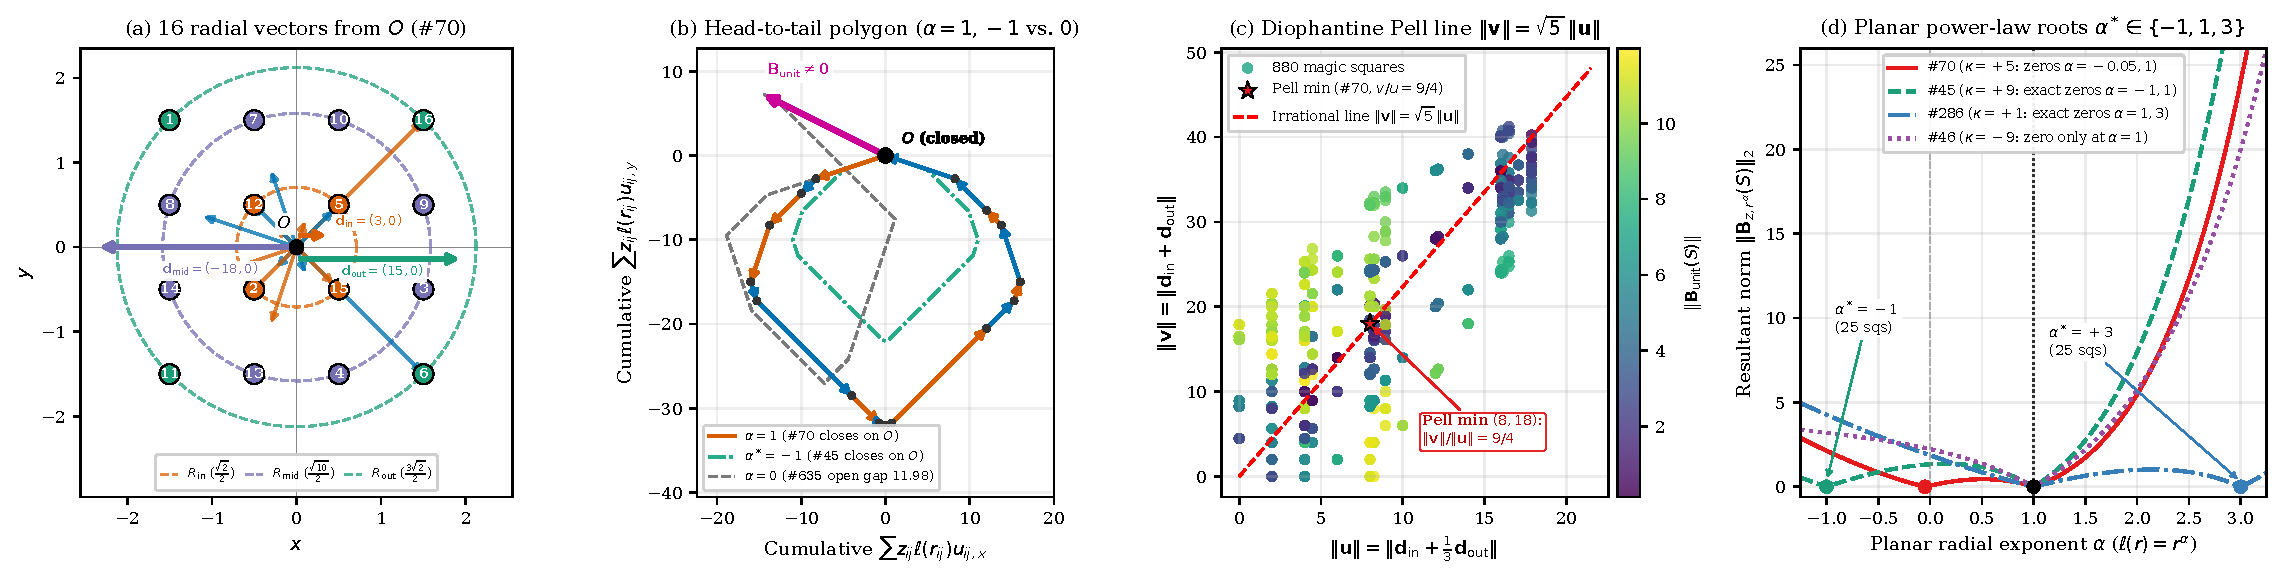
\includegraphics[width=\textwidth]{figures/fig_ring_vectors.pdf}
\caption{Planar radial vectors from the origin $O=(0,0)$, head-to-tail polygon closure, and the Diophantine Pell minimum at order four. (a)~The $16$ radial vectors $z_{ij}\mathbf r_{ij}$ radiating from $O$ (orange $z_{ij}>0$ outward, blue $z_{ij}<0$ inward) across the three concentric rings $R_{\mathrm{in}},R_{\mathrm{mid}},R_{\mathrm{out}}$ on square \#70, together with the three ring dipole resultants $\mathbf d_{\mathrm{in}}=(3,0)$, $\mathbf d_{\mathrm{out}}=(15,0)$, and $\mathbf d_{\mathrm{mid}}=(-18,0)$. (b)~Placing the $16$ vectors $z_{ij}\ell(r_{ij})\mathbf u_{ij}$ head-to-tail in order of angle around $O$ produces a closed $16$-gon at linear lengths $\alpha=1$ ($\ell(r)=r$ on \#70, solid orange/blue) and at inverse radial lengths $\alpha^*=-1$ ($\ell(r)=1/r$ on \#45, green dash-dot), whereas unit lengths $\alpha=0$ ($\ell(r)=1$ on \#635, dashed) fail to close by the magenta gap vector $\mathbf B_{\mathrm{unit}}(S)$. (c)~Scatter plot of $\|\mathbf v(S)\|_2=\|\mathbf d_{\mathrm{in}}+\mathbf d_{\mathrm{out}}\|_2$ versus $\|\mathbf u(S)\|_2=\|\mathbf d_{\mathrm{in}}+\frac13\mathbf d_{\mathrm{out}}\|_2$ across all $880$ magic squares against the irrational balance line $\|\mathbf v\|=\sqrt{5}\,\|\mathbf u\|$, with the eight Pell-minimum squares ($v/u=9/4$) marked by red stars. (d)~Resultant norm $\|\mathbf B_{z,r^\alpha}(S)\|_2$ versus power-law exponent $\alpha$, highlighting the universal root at $\alpha=1$ and the exact second roots at $\alpha^*=-1$ (\#45, $\kappa=+9$), $\alpha^*=-0.050$ (\#70, $\kappa=+5$), and $\alpha^*=+3$ (\#286, $\kappa=+1$).}
\label{fig:ring-vectors}
\end{figure}

\begin{theorem}[Three-Ring Decomposition, Irrationality No-Go, and Pell Minimum]
\label{thm:three-ring}
For any arrangement $S$ of order $4$, define the three ring dipole vectors radiating from $O$:
\[
\mathbf d_{\mathrm{in}}(S) = \sum_{c\in R_{\mathrm{in}}} z_c\mathbf r_c,\qquad
\mathbf d_{\mathrm{mid}}(S) = \sum_{c\in R_{\mathrm{mid}}} z_c\mathbf r_c,\qquad
\mathbf d_{\mathrm{out}}(S) = \sum_{c\in R_{\mathrm{out}}} z_c\mathbf r_c.
\]
\begin{enumerate}
\item \emph{(Ring sums, integrality, and non-vanishing.)} For every $4\times4$ arrangement $S$ of distinct integers, $\mathbf d_{\mathrm{in}}(S)\ne\mathbf 0$ and $\mathbf d_{\mathrm{out}}(S)\ne\mathbf 0$. For every order-four magic square $S\in\mathcal M_4$, both $R_{\mathrm{in}}$ and $R_{\mathrm{out}}$ sum to $\mu_4=34$ (so $\sum_{c\in R_{\mathrm{in}}}z_c=\sum_{c\in R_{\mathrm{out}}}z_c=0$), and hence $\mathbf d_{\mathrm{in}}(S)\in\Z^2\setminus\{\mathbf 0\}$ and $\mathbf d_{\mathrm{out}}(S)\in(3\Z)^2\setminus\{\mathbf 0\}$, with
\begin{equation}
\label{eq:ring-lower}
\|\mathbf d_{\mathrm{in}}(S)\|_2 \ge 1,\qquad \|\mathbf d_{\mathrm{out}}(S)\|_2 \ge 3.
\end{equation}
\item \emph{(Three-ring formula.)} Whenever $\sum_{c\in A_4}z_c\mathbf r_c=\mathbf 0$ (in particular, for every semi-magic square), $\mathbf d_{\mathrm{mid}}(S)=-\bigl(\mathbf d_{\mathrm{in}}(S)+\mathbf d_{\mathrm{out}}(S)\bigr)$, and for every radial length profile $\ell=(\ell_1,\ell_2,\ell_3)$ on $(r_1,r_2,r_3)$,
\begin{equation}
\label{eq:three-ring-general}
\mathbf B_{z,\ell}(S) = \left(\frac{\ell_1}{r_1} - \frac{\ell_2}{r_2}\right)\mathbf d_{\mathrm{in}}(S)
+ \left(\frac{\ell_3}{r_3} - \frac{\ell_2}{r_2}\right)\mathbf d_{\mathrm{out}}(S).
\end{equation}
\item \emph{(No-go theorem for unit vectors and even power laws.)} For planar unit vectors ($\ell_1=\ell_2=\ell_3=1$, i.e.\ $\alpha=0$), substituting $1/r_1=\sqrt{2}$, $1/r_3=\sqrt{2}/3$, and $1/r_2=\sqrt{2}/\sqrt{5}$ into \eqref{eq:three-ring-general} separates the rational $\sqrt{2}$ coefficients from the irrational $\sqrt{2}/\sqrt{5}$ coefficient:
\begin{equation}
\label{eq:unit-uv}
\mathbf B_{\mathrm{unit}}(S) = \sqrt{2}\,\left(\mathbf u(S) - \frac{1}{\sqrt{5}}\,\mathbf v(S)\right),
\end{equation}
where $\mathbf u(S)=\mathbf d_{\mathrm{in}}(S)+\frac13\mathbf d_{\mathrm{out}}(S)\in\Z^2$ collects the inner and outer ring contributions and $\mathbf v(S)=\mathbf d_{\mathrm{in}}(S)+\mathbf d_{\mathrm{out}}(S)=-\mathbf d_{\mathrm{mid}}(S)\in\Z^2$ is the negative middle-ring dipole. Because $\sqrt{5}\notin\Q$ and $\mathbf d_{\mathrm{in}}(S),\mathbf d_{\mathrm{out}}(S)\ne\mathbf 0$, \emph{no $4\times4$ arrangement of distinct integers with vanishing first moments (and hence no $4\times4$ semi-magic or magic square) ever satisfies $\mathbf B_{\mathrm{unit}}(S)=\mathbf 0$}, nor can $\mathbf B_{z,r^\alpha}(S)=\mathbf 0$ hold for any even integer $\alpha\in2\Z$.
\item \emph{(Exact Diophantine Pell minimum over $\mathcal M_4$.)} Across all $880$ magic squares of order~$4$, the global minimum of $\|\mathbf B_{\mathrm{unit}}(S)\|_2$ is
\begin{equation}
\label{eq:pell-min}
\min_{S\in\mathcal M_4} \|\mathbf B_{\mathrm{unit}}(S)\|_2
= \frac{18\sqrt{10}}{5} - 8\sqrt{2}
= \frac{2\sqrt{10}}{5(9+4\sqrt{5})}
= \frac{2\sqrt{10}}{5\varphi^6} \approx 0.07049108,
\end{equation}
where $\varphi=(1+\sqrt{5})/2$. This minimum is attained when $\mathbf d_{\mathrm{out}}(S)=5\mathbf d_{\mathrm{in}}(S)$ with $\|\mathbf d_{\mathrm{in}}(S)\|_2=3$, where $\mathbf u(S)$ and $\mathbf v(S)$ are parallel in the ratio $\|\mathbf v\|/\|\mathbf u\|=18/8=9/4$, the fundamental Pell convergent to $\sqrt{5}$ ($9^2-5\cdot4^2=1$). Up to $D_4$-symmetry, exactly eight magic squares achieve \eqref{eq:pell-min}: squares \#70, \#76, \#121, \#188, \#452, \#459, \#490, and \#574, all in Dudeney's Group~VI.
\end{enumerate}
\end{theorem}

\begin{proof}
(1) Labelling the four entries of $R_{\mathrm{in}}$ at $(-\frac12,\frac12)$, $(\frac12,\frac12)$, $(-\frac12,-\frac12)$, $(\frac12,-\frac12)$ by $a,b,c,d\in\Z$ gives $\mathbf d_{\mathrm{in}}(S)=\frac12\bigl((b+d)-(a+c),(a+b)-(c+d)\bigr)$. If $\mathbf d_{\mathrm{in}}(S)=\mathbf 0$, then $b+d=a+c$ and $a+b=c+d$; adding and subtracting these equations forces $b=c$ and $a=d$, contradicting that $S$ has distinct entries. For $S\in\mathcal M_4$, subtracting the sum of all $16$ cells ($4\mu_4$) from the sum of the two outer rows and two outer columns ($R_0+R_3+C_0+C_3=4\mu_4$) gives $\sum_{c\in R_{\mathrm{out}}}s_c-\sum_{c\in R_{\mathrm{in}}}s_c=0$, while the two main diagonals sum to $D_1+D_2=\sum_{c\in R_{\mathrm{out}}}s_c+\sum_{c\in R_{\mathrm{in}}}s_c=2\mu_4$; hence $\sum_{c\in R_{\mathrm{in}}}s_c=\sum_{c\in R_{\mathrm{out}}}s_c=\mu_4=34$ (an even integer), which implies $\mathbf d_{\mathrm{in}}(S)\in\Z^2\setminus\{\mathbf 0\}$. Since the corner coordinates are $(\pm\frac32,\pm\frac32)=3(\pm\frac12,\pm\frac12)$, identical algebra gives $\mathbf d_{\mathrm{out}}(S)\in(3\Z)^2\setminus\{\mathbf 0\}$ and \eqref{eq:ring-lower}.

(2) Partitioning $A_4=R_{\mathrm{in}}\sqcup R_{\mathrm{mid}}\sqcup R_{\mathrm{out}}$ gives $\mathbf d_{\mathrm{mid}}=-(\mathbf d_{\mathrm{in}}+\mathbf d_{\mathrm{out}})$, and substituting this relation into \eqref{eq:B-planar} yields \eqref{eq:three-ring-general}.

(3) Setting $\ell_1=\ell_2=\ell_3=1$ with $1/r_1=\sqrt{2}$, $1/r_2=\sqrt{2}/\sqrt{5}$, and $1/r_3=\sqrt{2}/3$ in \eqref{eq:three-ring-general} gives $\mathbf B_{\mathrm{unit}}(S)=(\sqrt{2}-\sqrt{2}/\sqrt{5})\mathbf d_{\mathrm{in}}+(\sqrt{2}/3-\sqrt{2}/\sqrt{5})\mathbf d_{\mathrm{out}}=\sqrt{2}\bigl((\mathbf d_{\mathrm{in}}+\frac13\mathbf d_{\mathrm{out}})-\frac{1}{\sqrt{5}}(\mathbf d_{\mathrm{in}}+\mathbf d_{\mathrm{out}})\bigr)$, which is \eqref{eq:unit-uv}. Because $\mathbf u(S),\mathbf v(S)\in\Z^2$ by~(1) and $\sqrt{5}\notin\Q$, $\mathbf B_{\mathrm{unit}}(S)=\mathbf 0$ requires $\mathbf u(S)=\mathbf v(S)=\mathbf 0$, which forces $\mathbf d_{\mathrm{in}}(S)=\mathbf d_{\mathrm{out}}(S)=\mathbf 0$, contradicting~(1). The same irrationality holds for any even exponent $\alpha=2m$, where $r_2^{\alpha-1}/r_1^{\alpha-1}=5^{m-1}\sqrt{5}\notin\Q$.

(4) Since $\mathbf v(S)-\mathbf u(S)=\frac23\mathbf d_{\mathrm{out}}(S)\in(2\Z)^2$, the integer vectors satisfy the parity congruence $\mathbf u(S)\equiv\mathbf v(S)\pmod 2$ for every semi-magic square, while $\mathbf d_{\mathrm{in}},\mathbf d_{\mathrm{out}}\ne\mathbf 0$ implies $\mathbf u\ne\mathbf v$ and $\mathbf v\ne 3\mathbf u$. Decomposing $\mathbf v$ parallel and orthogonal to $\mathbf u$ shows that $\|\mathbf u-\mathbf v/\sqrt{5}\|_2$ is minimized when $\mathbf u=p\mathbf e$ and $\mathbf v=q\mathbf e$ are collinear along a primitive lattice direction $\mathbf e=(a,b)\in\Z^2$ ($\gcd(a,b)=1$), where $\|\mathbf B_{\mathrm{unit}}(S)\|_2=\sqrt{2(a^2+b^2)}\,|p-q/\sqrt{5}|$ and the prefactor $\sqrt{2(a^2+b^2)}$ is minimal along the coordinate axes ($a^2+b^2=1$). Over all integer pairs with $p\equiv q\pmod 2$, the best approximations to $\sqrt{5}$ are governed by the Pell--Lucas equation $q^2-5p^2=\pm 4$, whose positive solutions $(p,q)=(F_k,L_k)$ alternate between odd--odd Fibonacci--Lucas semiconvergents such as $(3,7)$, $(5,11)$, $(13,29)$, $(21,47)$ ($k\not\equiv 0\pmod 3$) and even--even pairs $(F_{3m},L_{3m})=2(p_m,q_m)$ obtained by doubling the principal continued-fraction convergents $q_m/p_m\in\{2/1,9/4,38/17,\dots\}$ of $\sqrt{5}=[2;\overline{4}]$. On $\mathcal M_4$, every pair $(F_k,L_k)$ with $k\ge 7$ is excluded on two independent grounds:
\begin{enumerate}
\item[(i)] \emph{Direct axial collinear bound:} Since $\frac13\mathbf d_{\mathrm{out}}=\frac12(\mathbf v-\mathbf u)$ and $\mathbf d_{\mathrm{in}}=\frac12(3\mathbf u-\mathbf v)$, realizing $(p,q)=(F_k,L_k)$ along a coordinate axis requires $\frac13|d_{\mathrm{out}}|=\frac12(L_k-F_k)$. Across $\mathcal M_4$, $\frac13\|\mathbf d_{\mathrm{out}}\|_\infty\le 12$, which immediately excludes all $k\ge 8$ ($\frac12(L_k-F_k)\ge\frac12(47-21)=13>12$). For $k=7$, $(F_7,L_7)=(13,29)$ requires $\frac13|d_{\mathrm{out}}|=\frac12(29-13)=8$ and $|d_{\mathrm{in}}|=\frac12(39-29)=5$; however, saturating $\frac13|d_{\mathrm{out}}|=8$ along a coordinate axis on $\mathcal M_4$ constrains the inner-ring dipole on every axial collinear square ($\mathbf d_{\mathrm{in}}\parallel\mathbf d_{\mathrm{out}}$) to $|d_{\mathrm{in}}|\le 4$ and hence $p=|d_{\mathrm{in}}+\frac13d_{\mathrm{out}}|\le 12<13$.
\item[(ii)] \emph{Even-lattice property:} Subtracting $C_1+C_2=2\mu_4$ and $C_0+C_3=2\mu_4$ from $D_1+D_2=2\mu_4$ gives $s_{00}+s_{03}=s_{31}+s_{32}$ and $s_{11}+s_{12}=s_{20}+s_{23}$, and across all $24$ modulo-$2$ parity patterns of $\mathcal M_4$ the four top diagonal cells $T_{\mathrm{diag}}=\{(0,0),(0,3),(1,1),(1,2)\}$ (and likewise $R_{\mathrm{diag}}=\{(0,3),(3,3),(1,2),(2,2)\}$) always have an even sum $\sum_{c\in T_{\mathrm{diag}}}s_c\in\{18,20,\dots,42\}$. Because $u_y(S)=\sum_{c\in T_{\mathrm{diag}}}s_c-34$ and $u_x(S)=\sum_{c\in R_{\mathrm{diag}}}s_c-34$, every magic square $S\in\mathcal M_4$ satisfies
\[
\mathbf u(S) = 2\tilde{\mathbf u}(S) \in (2\Z)^2,\enspace
\mathbf v(S) = 2\tilde{\mathbf v}(S) \in (2\Z)^2,\enspace
\|\mathbf u(S)\|_\infty \le 16,\enspace
\|\mathbf u(S)\|_2 \le 8\sqrt{5} \approx 17.89,
\]
excluding all odd--odd Pell--Lucas pairs and reducing \eqref{eq:unit-uv} to $\|\mathbf B_{\mathrm{unit}}(S)\|_2=2\sqrt{2}\,\|\tilde{\mathbf u}(S)-\tilde{\mathbf v}(S)/\sqrt{5}\|_2$ with $\tilde{\mathbf u}(S),\tilde{\mathbf v}(S)\in\Z^2$ and $\|\tilde{\mathbf u}(S)\|_2\le 4\sqrt{5}<9$.
\end{enumerate}
By Lagrange's theorem on continued fractions, across all integer denominators $1\le\tilde u<17$, the unique best rational approximation to $\sqrt{5}$ is the fundamental Pell convergent $\tilde v/\tilde u=9/4$ ($9^2-5\cdot 4^2=1$), corresponding to $(p,q)=(F_6,L_6)=(8,18)$ and giving $2\sqrt{2}(9/\sqrt{5}-4)=18\sqrt{10}/5-8\sqrt{2}=2\sqrt{10}/(5\varphi^6)\approx0.07049108$ (since $\varphi^6=(2+\sqrt{5})^2=9+4\sqrt{5}$), whereas the next convergent $38/17$ requires $\|\tilde{\mathbf u}\|_2\ge 17>4\sqrt{5}$. On square \#70 (\Cref{fig:hero-squares}(b)), the inner ring $\{5,12,2,15\}$ gives $\mathbf d_{\mathrm{in}}=\frac12\bigl((12+15)-(5+2),(12+5)-(2+15)\bigr)=(3,0)$ and the outer corners $\{1,16,11,6\}$ give $\mathbf d_{\mathrm{out}}=\frac32\bigl((16+6)-(1+11),(1+16)-(11+6)\bigr)=(15,0)=5\mathbf d_{\mathrm{in}}$, realizing $\mathbf u=(8,0)$, $\mathbf v=(18,0)$, and \eqref{eq:pell-min}.
\end{proof}

How, then, can a planar balance wheel achieve exact equilibrium at a non-linear length profile $\ell(r)=r^\alpha$ ($\alpha\ne1$)? Equation~\eqref{eq:three-ring-general} shows that balance is restored whenever the inner and outer ring dipoles align in the same direction ($\mathbf d_{\mathrm{out}}=\kappa\mathbf d_{\mathrm{in}}$ with $\kappa>0$), so that both rings jointly oppose the middle ring $\mathbf d_{\mathrm{mid}}=-(1+\kappa)\mathbf d_{\mathrm{in}}$ (\Cref{fig:ring-vectors}(d)).

\begin{corollary}[Restoring planar balance via power-law exponents $\alpha^*\ne1$]
\label{cor:planar-power-roots}
For power-law radial lengths $\ell(r)=r^\alpha$ ($\alpha\in\R$), equation~\eqref{eq:three-ring-general} takes the form
\begin{equation}
\label{eq:planar-power-form}
\mathbf B_{z,r^\alpha}(S) = r_1^{\alpha-1}\Bigl[\bigl(1 - 5^{(\alpha-1)/2}\bigr)\mathbf d_{\mathrm{in}}(S) + \bigl(3^{\alpha-1} - 5^{(\alpha-1)/2}\bigr)\mathbf d_{\mathrm{out}}(S)\Bigr].
\end{equation}
\begin{enumerate}
\item Because $1<\sqrt{5}<3$, the ratio $h(\alpha)=\frac{5^{(\alpha-1)/2}-1}{3^{\alpha-1}-5^{(\alpha-1)/2}}$ (extended by $h(1)=\frac{\ln 5}{\ln(9/5)}\approx2.7381$) is a strictly decreasing bijection from $\R$ onto $(0,\infty)$. Consequently, an order-four magic square $S$ possesses a second power-law balance exponent $\alpha^*(S)\ne1$ satisfying $\mathbf B_{z,r^{\alpha^*}}(S)=\mathbf 0$ if and only if $\mathbf d_{\mathrm{in}}(S)$ and $\mathbf d_{\mathrm{out}}(S)$ are strictly parallel ($\mathbf d_{\mathrm{out}}(S)=\kappa\mathbf d_{\mathrm{in}}(S)$ with $\kappa>0$), which holds for $204$ of the $880$ magic squares (while $204$ squares have anti-parallel dipoles $\kappa<0$).
\item Across all $880$ magic squares, the second root $\alpha^*(\kappa)$ is an integer in only two cases:
\begin{itemize}
\item $\alpha^*=-1$ (inverse radial lengths $\ell(r)=1/r$), corresponding to $\kappa=h(-1)=+9$, achieved by $25$ squares (e.g.\ square \#45 in \Cref{fig:hero-squares}(c), where $\mathbf d_{\mathrm{in}}=(0,-2)$ and $\mathbf d_{\mathrm{out}}=(0,-18)=9\mathbf d_{\mathrm{in}}$);
\item $\alpha^*=+3$ (cubic radial lengths $\ell(r)=r^3$), corresponding to $\kappa=h(3)=+1$, achieved by $25$ squares (e.g.\ square \#286).
\end{itemize}
For the $17$ squares with $\kappa=+5$ (including the eight Pell-minimum squares of \Cref{thm:three-ring}(4)), the exact zero occurs at $\alpha^*(5)\approx -0.0496$, explaining why $\|\mathbf B_{z,r^\alpha}(S)\|_2$ pinches nearly to zero at $\alpha=0$ (\Cref{fig:ring-vectors}(d)).
\end{enumerate}
\end{corollary}

\begin{proof}
Setting \eqref{eq:planar-power-form} to $\mathbf 0$ for $\alpha\ne1$ requires $\mathbf d_{\mathrm{out}}(S)=h(\alpha)\mathbf d_{\mathrm{in}}(S)$. Since $1<5^{t/2}<3^t$ for $t=\alpha-1>0$ and $3^t<5^{t/2}<1$ for $t<0$, both numerator and denominator of $h(\alpha)$ have the sign of $\alpha-1$, so $h(\alpha)>0$ with $\lim_{\alpha\to-\infty}h(\alpha)=+\infty$ and $\lim_{\alpha\to+\infty}h(\alpha)=0$. Since $\kappa\in\Q_{>0}$ cannot equal the transcendental number $\frac{\ln 5}{\ln(9/5)}$, every square with $\kappa>0$ has a unique root $\alpha^*(\kappa)=h^{-1}(\kappa)\ne1$. By \Cref{thm:three-ring}(3), an integer root $\alpha^*\ne1$ must be odd, $\alpha^*=2m+1$ ($m\in\Z\setminus\{0\}$), where $h(2m+1)=\frac{5^m-1}{9^m-5^m}$; comparing this sequence against the $15$ positive rational ratios $\kappa$ realized on $\mathcal M_4$ leaves only $m=-1$ ($\kappa=9$, $25$ squares) and $m=+1$ ($\kappa=1$, $25$ squares).
\end{proof}

\subsection{Three-Dimensional Spoke Stars: Unit-Sphere Counterweights and Cubic Vertical Balance}

We now lift the spoke sculpture into three dimensions (\Cref{fig:origin-vectors-3d}). In 3D, trimming all $16$ spokes to the unit sphere $S^2$ ($\beta=0$) breaks equilibrium on $832$ of the $880$ squares, sparing only the $48$ associative squares of Group~III where antipodal pairs cancel pairwise ($\hat{\mathbf p}_{-c}=-\hat{\mathbf p}_c$). Nevertheless, because the natural unequal lengths $R_{ij}(\lambda)>0$ satisfy $\sum_{i,j}R_{ij}(\lambda)\hat{\mathbf p}_{ij}(\lambda)=\mathbf 0$, the origin $O$ always lies strictly inside the convex hull of the $16$ unit rays, guaranteeing that positive unequal tip weights $\mathbf w^*>\mathbf 0$ restore unit-sphere equilibrium for every magic square.

\begin{figure}[htbp]
\centering
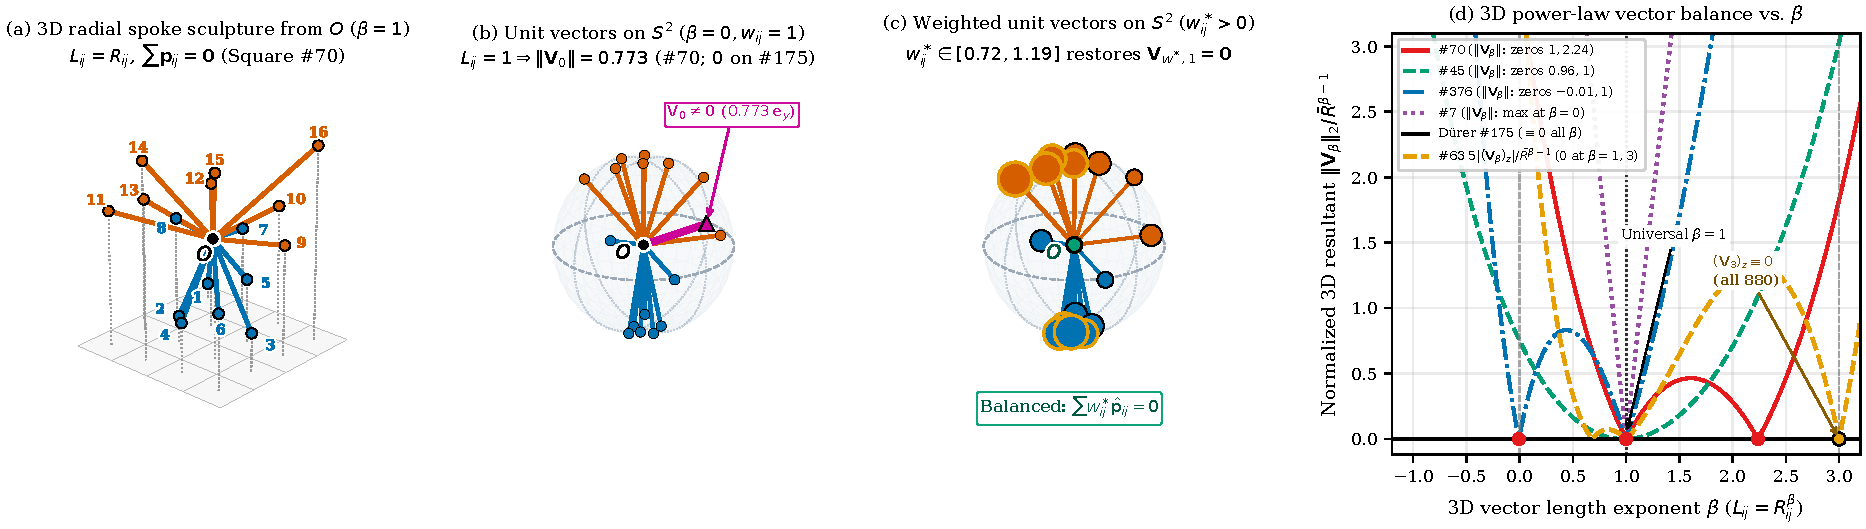
\includegraphics[width=\textwidth]{figures/fig_origin_vectors_3d.pdf}
\caption{Three-dimensional radial spoke sculptures from the origin $O=(0,0,0)$ of variable length and tip weight. (a)~The $16$-spoke radial sculpture $\mathbf p_{ij}$ ($\beta=1$, spoke length $L_{ij}=R_{ij}$, orange for $z_{ij}>0$, blue for $z_{ij}<0$) of non-associative square \#70 over the floor grid, balancing identically at the central hub $O$ ($\sum\mathbf p_{ij}=\mathbf 0$). (b)~Trimming all $16$ spokes to unit length $L_{ij}=1$ ($\beta=0$, equal tip weights $w_{ij}=1$) on the unit sphere $S^2$ leaves a non-zero resultant $\mathbf V_0=(0,0.773,0)$ (magenta arrow) on square \#70, whereas antipodal pairs cancel on associative D\"urer \#175. (c)~Assigning the minimum-variance positive tip weights $w_{ij}^*\in[0.72,1.19]$ (sphere tip sizes, gold-rimmed for $w_{ij}^*>1$) restores exact unit-sphere balance $\sum w_{ij}^*\hat{\mathbf p}_{ij}=\mathbf 0$ at $O$. (d)~Normalized 3D power-law resultant $\|\mathbf V_\beta(S;1)\|_2/\bar R^{\beta-1}$ versus length exponent $\beta$, showing universal balance at $\beta=1$, second power-law roots $\beta^*\ne1$ on Group~VI squares (\#70 at $\beta^*=2.24$, \#45 at $0.96$, \#376 at $-0.008$), and identical vertical vanishing $(\mathbf V_3)_z=0$ at $\beta=3$ (gold dashed curve showing $5|(\mathbf V_\beta)_z|/\bar R^{\beta-1}$ on square \#63).}
\label{fig:origin-vectors-3d}
\end{figure}

\begin{theorem}[3D Power-Law Vectors, Cubic Vertical Vanishing, and Positive Unit-Sphere Weights]
\label{thm:3d-power}
Let $S$ be a semi-magic square of order $n$ and let $\lambda>0$.
\begin{enumerate}
\item \emph{(Cubic 3D vector law $\beta=3$.)} For cubic 3D spoke lengths $L_{ij}=R_{ij}(\lambda)^3$ from the origin (dual by \Cref{prop:reciprocity}(1) to weighting $\mathbf p_{ij}(\lambda)$ by $w_{ij}=R_{ij}(\lambda)^2=r_{ij}^2+\lambda^2z_{ij}^2$), the vertical $z$-component vanishes identically for every semi-magic square of any order $n$ and every $\lambda>0$:
\begin{equation}
\label{eq:V3-exact}
\mathbf V_3(S;\lambda) = \sum_{i,j}\bigl(r_{ij}^2+\lambda^2z_{ij}^2\bigr)(x_j,y_i,\lambda z_{ij})
= \biggl(\lambda^2\sum_{i,j}z_{ij}^2 x_j,\;\; \lambda^2\sum_{i,j}z_{ij}^2 y_i,\;\; 0\biggr).
\end{equation}
At order $n=4$, $\mathbf V_3(S;\lambda)=\mathbf 0$ if and only if $S$ is one of the $48$ associative magic squares.
\item \emph{(Unit-sphere parity and Group~VI power-law roots.)} Under any even weight function $w_{ij}=f(|z_{ij}|)$, every associative square satisfies $\hat{\mathbf p}_{-c}(\lambda)=-\hat{\mathbf p}_c(\lambda)$ and hence $\mathbf V_\beta(S;\lambda)=\mathbf 0$ for all $\beta\in\R$ and $\lambda>0$. At $n=4$, $\mathbf V_0(S;\lambda)=\mathbf 0$ holds if and only if $S$ is one of the $48$ associative squares ($\|\mathbf V_0(S;1)\|_2\in[0.0072,2.4284]$ on the remaining $832$ squares). Among the $304$ Group~VI squares (where $C_2$ symmetry confines $\mathbf V_\beta(S;\lambda)$ to a single coordinate axis), $107$ squares possess a second 3D power-law balance exponent $\beta^*(S)\in[-3,4]\setminus\{1\}$ with $\mathbf V_{\beta^*}(S;1)=\mathbf 0$ (\Cref{fig:origin-vectors-3d}(d)).
\item \emph{(Universal positive minimum-variance balancing weights on $S^2$.)} Letting $\hat P(\lambda)\in\R^{N\times 3}$ have rows $\hat{\mathbf p}_{ij}(\lambda)^{\top}$, the unique weight vector $\mathbf w^*(S;\lambda)$ of minimum Euclidean distance $\|\mathbf w-\mathbf 1\|_2$ from uniform weights $\mathbf 1$ satisfying $\sum_{i,j}w_{ij}^*\hat{\mathbf p}_{ij}(\lambda)=\mathbf 0$ is
\begin{equation}
\label{eq:w-star}
\mathbf w^*(S;\lambda) = \mathbf 1 - \hat P(\lambda)\bigl(\hat P(\lambda)^{\top}\hat P(\lambda)\bigr)^{-1}\mathbf V_0(S;\lambda).
\end{equation}
Across all $880$ order-four magic squares at $\lambda=1$, $\lambda_{\mathrm{iso}}=1/\sqrt{17}$, and $\lambda_{\mathrm{cube}}=0.20$, every square admits strictly positive optimal weights $\mathbf w^*(S;\lambda)>\mathbf 0$ (\Cref{fig:origin-vectors-3d}(c)), with $\|\mathbf w^*(S;1)-\mathbf 1\|_2\in[0.0052,\,1.5967]$ across the $832$ non-associative squares.
\end{enumerate}
\end{theorem}

\begin{proof}
(1) Expanding $\mathbf V_3(S;\lambda)=\sum_{i,j}(r_{ij}^2+\lambda^2z_{ij}^2)(x_j,y_i,\lambda z_{ij})$, the horizontal sum $\sum_{i,j}r_{ij}^2(x_j,y_i)$ vanishes by odd grid symmetry, leaving $\lambda^2\sum_{i,j}z_{ij}^2(x_j,y_i)$. The vertical component is $\lambda\sum_{i,j}(x_j^2+y_i^2)z_{ij}+\lambda^3\sum_{i,j}z_{ij}^3$; here $\sum_{i,j}(x_j^2+y_i^2)z_{ij}=0$ because $x_j^2+y_i^2\in W_{\mathrm{rc}}$, and $\sum_{i,j}z_{ij}^3=0$ by odd symmetry of $\{z_{ij}\}$, proving \eqref{eq:V3-exact}.

(2) For associative squares, $z(-x,-y)=-z(x,y)$ implies $\mathbf p_{-c}(\lambda)=-\mathbf p_c(\lambda)$ and $R_{-c}(\lambda)=R_c(\lambda)$, so opposite cells cancel pairwise for every $\beta\in\R$.

(3) Minimizing $\frac12\|\mathbf w-\mathbf 1\|_2^2$ subject to $\hat P(\lambda)^{\top}\mathbf w=\mathbf 0$ by Lagrange multipliers gives \eqref{eq:w-star}, and exact enumeration over the $880$ squares establishes positivity and the stated bounds.
\end{proof}

Notice how the cubic resultant $\mathbf V_3(S;\lambda)$ in \eqref{eq:V3-exact} bridges static rays and rotational dynamics: while its vertical component vanishes for every semi-magic square, its residual horizontal dipole $\lambda^2\sum_{i,j}z_{ij}^2(x_j,y_i)$ measures the quadratic height asymmetry across the grid. In Test~2, we set our sculptures into three-dimensional rotation and see that this exact vector governs the vertical off-diagonal products of inertia of an entry-weighted gem.

\section{Test 2: Rotational Dynamics---Equal Masses Precess, Entry Masses Flip}
\label{sec:dynamics}

Our second test moves from static radial equilibrium to three-dimensional rotation. Suppose a Magic Gem or radial spoke sculpture of total mass $M$ and centre of mass $\mathbf c$ is supported on a low-friction conical pivot or gimbal at the origin $O$ under uniform gravity $\mathbf g=(0,0,-g)^{\top}$ (generalizing the conical fulcrum of \texttt{weighted\_ring.stl} in \cite{mathewson2025magicgemweb}), or tossed in free space. About the pivot $O$, gravity exerts the torque
\[
\boldsymbol\tau_{\mathrm{grav}} = M\,\mathbf c \times \mathbf g,
\]
which \emph{vanishes identically in every 3D orientation if and only if the centre of mass lies at the pivot ($\mathbf c=\mathbf 0$)}. Consequently, any balanced sculpture ($\mathbf c=\mathbf 0$) supported at $O$ rotates under Earth's gravity according to Euler's exact torque-free equations \cite{arnold1989mathematical,goldstein2002classical}: in the principal body frame, the angular velocity vector $\boldsymbol\omega=(\omega_1,\omega_2,\omega_3)^{\top}$ evolves via
\begin{equation}
\label{eq:euler}
I_1\dot\omega_1 = (I_2-I_3)\omega_2\omega_3,\qquad
I_2\dot\omega_2 = (I_3-I_1)\omega_3\omega_1,\qquad
I_3\dot\omega_3 = (I_1-I_2)\omega_1\omega_2,
\end{equation}
where $I_1,I_2,I_3$ are the principal moments of inertia. For an asymmetric body with three distinct principal moments $I_1<I_2<I_3$, rotation about the intermediate axis $I_2$ is exponentially unstable: any small perturbation grows at rate $\sqrt{(I_2-I_1)(I_3-I_2)/(I_1I_3)}\,|\omega_2|$, causing the body to execute the $180^\circ$ flips of the Dzhanibekov (or tennis-racket) theorem \cite{ashbaugh1991twisting,poinsot1834theorie}.

Test~2 asks: \emph{when the $16$ unequal heights $z_{ij}$ are set spinning in $\R^3$, do their geometric inequalities produce an asymmetric top that tumbles via Dzhanibekov flips, or does line-sum equality enforce smooth axisymmetric precession?}

\subsection{Equal Masses at Unequal Heights Form a Universal Axisymmetric Rotor}

Consider first the discrete point cloud $P_S(\lambda)=\{\mathbf p_{ij}(\lambda)=(x_j,y_i,\lambda z_{ij})\}$ carrying equal point masses $m=M/N$ at the $N=n^2$ unequal lifted points (for instance, identical steel bearings mounted at the tips of the sixteen radial spokes $\mathbf p_{ij}(\lambda)$ on a lightweight hub at $O$). Because $\mathbf c=\frac1N\sum_{i,j}\mathbf p_{ij}(\lambda)=\mathbf 0$, gravitational torque about $O$ vanishes identically for every semi-magic square, and the magic line sums neutralize all off-diagonal products of inertia.

\begin{theorem}[Universal symmetric-top law, spherical-top scale, and periodic polhodes]
\label{thm:rotor}
Let $S$ be any arrangement of $\{1,\dots,n^2\}$ ($n\ge2$) whose height field has vanishing first moments $\sum_{i,j}x_jz_{ij}=\sum_{i,j}y_iz_{ij}=0$ (in particular, any semi-magic or magic square), and place equal point masses $m=M/N$ at the points $\mathbf p_{ij}(\lambda)=(x_j,y_i,\lambda z_{ij})$.
\begin{enumerate}
\item \emph{(Axisymmetric inertia tensor.)} For every $\lambda>0$, the inertia tensor about the origin $O$,
\[
I(\lambda) = \frac{M}{N}\sum_{i,j}\Bigl(\|\mathbf p_{ij}(\lambda)\|_2^2\,I_3 - \mathbf p_{ij}(\lambda)\mathbf p_{ij}(\lambda)^{\top}\Bigr),
\]
is diagonal and strictly axisymmetric about the $z$-axis:
\begin{equation}
\label{eq:inertia-point}
I(\lambda) = M\diag\bigl(I_\perp(\lambda),\, I_\perp(\lambda),\, I_{zz}\bigr),\qquad
I_\perp(\lambda) = a_n + \lambda^2 b_n,\qquad
I_{zz} = 2a_n,
\end{equation}
with universal principal inertia ratio
\begin{equation}
\label{eq:inertia-ratio}
\frac{I_\perp(\lambda)}{I_{zz}} = \frac{a_n + \lambda^2 b_n}{2a_n} = \frac{1 + \lambda^2(n^2+1)}{2}.
\end{equation}
\item \emph{(Three critical aspect ratios.)} Varying the vertical lift scale $\lambda$ drives the rotor through three regimes (\Cref{fig:precession}(a)):
\begin{enumerate}
\item At the \emph{canonical lift} $\lambda=1$,
\begin{equation}
\label{eq:ratio-lambda1}
\frac{I_\perp(1)}{I_{zz}} = \frac{n^2+2}{2},
\end{equation}
which is an exact integer for every even order $n$ ($9$ for $n=4$, $19$ for $n=6$, $33$ for $n=8$) and a half-integer for every odd order $n$ ($11/2$ for $n=3$, $27/2$ for $n=5$).
\item At the \emph{spherical-top critical scale}
\begin{equation}
\label{eq:lambda-iso}
\lambda_{\mathrm{iso}}(n) = \frac{1}{\sqrt{n^2+1}}
\qquad\Bigl(\tfrac{1}{\sqrt{10}}\approx0.3162\text{ for }n=3,\quad \tfrac{1}{\sqrt{17}}\approx0.2425\text{ for }n=4\Bigr),
\end{equation}
$I_\perp(\lambda_{\mathrm{iso}})=I_{zz}=2a_n$, so $I(\lambda_{\mathrm{iso}})=2Ma_nI_3$ is a scalar multiple of the identity: the point-weighted gem is a \emph{spherical top} for which every axis through $O$ in $\R^3$ is a principal axis of inertia.
\item At the \emph{cubic bounding-box scale} $\lambda_{\mathrm{cube}}(n)=\frac{n-1}{n^2-1}=\frac{1}{n+1}$ (where the vertical span matches the horizontal footprint $[-\frac{n-1}{2},\frac{n-1}{2}]^2$, giving $\lambda_{\mathrm{cube}}=1/5=0.20$ at $n=4$),
\begin{equation}
\label{eq:ratio-cube}
\frac{I_\perp(\lambda_{\mathrm{cube}})}{I_{zz}} = \frac{n^2+n+1}{(n+1)^2}
\qquad\Bigl(\frac{21}{25}=0.84\text{ at }n=4\Bigr).
\end{equation}
\end{enumerate}
\item \emph{(Suppression of Dzhanibekov tumbling and rational orbit closure.)} Because $I_{xx}(\lambda)=I_{yy}(\lambda)=I_\perp(\lambda)$, no distinct intermediate principal axis exists. In torque-free motion \eqref{eq:euler}, $\omega_3(t)=\omega_{3,0}$ is constant and the transverse angular velocity $(\omega_1(t),\omega_2(t))$ precesses in a uniform circle at the body-frame polhode frequency
\begin{equation}
\label{eq:polhode-freq}
\Omega_{\mathrm{body}}(\lambda) = \frac{I_\perp(\lambda)-I_{zz}}{I_\perp(\lambda)}\,\omega_{3,0}
= \frac{\lambda^2(n^2+1)-1}{\lambda^2(n^2+1)+1}\,\omega_{3,0}.
\end{equation}
At $\lambda=1$, $\Omega_{\mathrm{body}}(1)=\frac{n^2}{n^2+2}\omega_{3,0}$ is a rational multiple of the spin rate $\omega_{3,0}$, so the polhode and space-cone trajectories close periodically after $n^2+2$ spin revolutions (or $(n^2+2)/2=9$ revolutions at $n=4$). At $\lambda=\lambda_{\mathrm{iso}}(n)$, $\Omega_{\mathrm{body}}=0$ and the gem rotates steadily without wobble about any initial angular velocity vector $\boldsymbol\omega_0\in\R^3$.
\end{enumerate}
\end{theorem}

\begin{proof}
By \cite[Lem.~3.1]{mathewson2026gems}, the empirical covariance matrix $\Sigma(\lambda)=\frac1N\sum_{i,j}\mathbf p_{ij}(\lambda)\mathbf p_{ij}(\lambda)^{\top}$ has diagonal entries $\Sigma_{xx}=\Sigma_{yy}=a_n=(n^2-1)/12$ and $\Sigma_{zz}=\lambda^2b_n=\lambda^2(n^4-1)/12=\lambda^2(n^2+1)a_n$, while $\Sigma_{xy}=0$ by grid symmetry and $\Sigma_{xz}=\Sigma_{yz}=0$ by vanishing of the first moments. Since $I(\lambda)=M\bigl(\tr(\Sigma(\lambda))I_3-\Sigma(\lambda)\bigr)$, we obtain \eqref{eq:inertia-point} and \eqref{eq:inertia-ratio}. Specializing \eqref{eq:inertia-ratio} to $\lambda=1$, $\lambda=(n^2+1)^{-1/2}$, and $\lambda=(n+1)^{-1}$ yields (2a)--(2c). Substituting $I_1=I_2=I_\perp(\lambda)$ and $I_3=I_{zz}$ into Euler's equations \eqref{eq:euler} gives $\dot\omega_3=0$ and $\dot\omega_1=\Omega_{\mathrm{body}}\omega_2$, $\dot\omega_2=-\Omega_{\mathrm{body}}\omega_1$ with $\Omega_{\mathrm{body}}$ as in \eqref{eq:polhode-freq}.
\end{proof}

\begin{figure}[htbp]
\centering
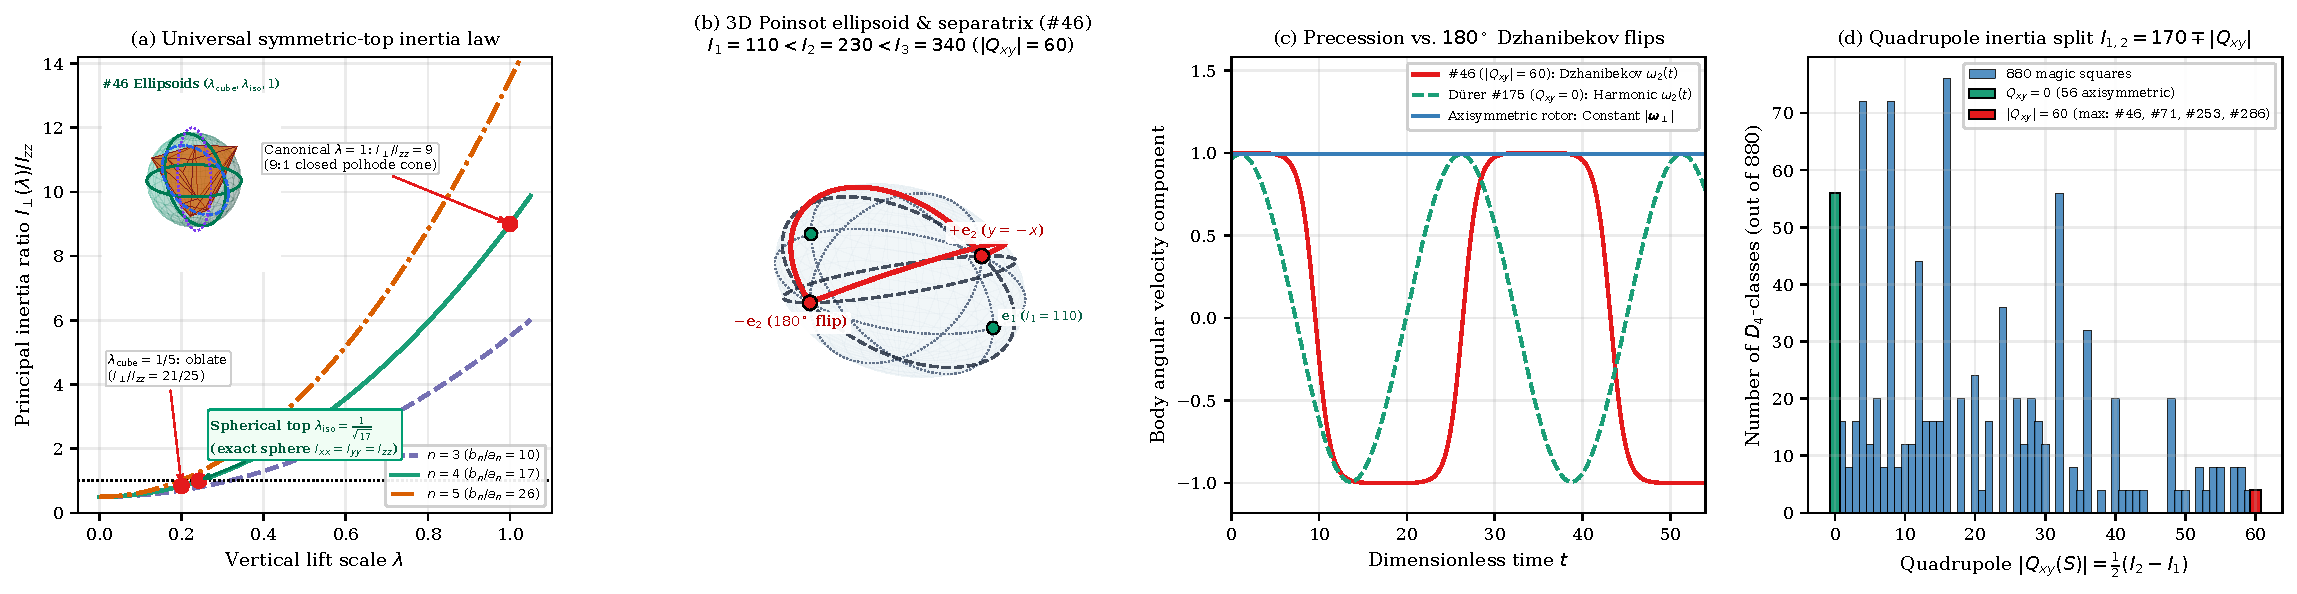
\includegraphics[width=\textwidth]{figures/fig_precession_dynamics.pdf}
\caption{Three-dimensional rotational dynamics of Magic Gems. (a)~Universal principal inertia ratio $I_\perp(\lambda)/I_{zz}=\frac12(1+\lambda^2(n^2+1))$ versus vertical scale $\lambda$ for orders $n=3,4,5$, with 3D inertia ellipsoids at the cubic 3D-print scale $\lambda_{\mathrm{cube}}=1/5$ ($21/25$), the isotropic spherical-top transition $\lambda_{\mathrm{iso}}=1/\sqrt{17}$ ($1$), and the canonical lift $\lambda=1$ ($9$) for $n=4$. (b)~Triaxial Poinsot energy ellipsoid $\frac12\sum I_k\omega_k^2=E$ of entry-weighted square \#46 ($I_1=110<I_2=230<I_3=340$), showing the figure-eight separatrix through the unstable intermediate saddle $\pm\boldsymbol\omega_2$ and the heteroclinic polhode orbit connecting $+\omega_2$ to $-\omega_2$. (c)~Time series of Euler's equations \eqref{eq:euler}: an axisymmetric magic rotor (D\"urer \#175 or any point-weighted gem) precesses harmonically with constant $|\boldsymbol\omega_\perp|$, whereas entry-weighted square \#46 ($|Q_{xy}|=60$) undergoes periodic $180^\circ$ Dzhanibekov flips $\omega_2(t)\in[+1,-1]$ about its intermediate diagonal axis. (d)~Census of the quadrupole moment $|Q_{xy}(S)|=|\sum z_{ij}x_jy_i|=\frac12(I_2-I_1)$ across the $880$ order-four magic squares.}
\label{fig:precession}
\end{figure}

\subsection{Unequal Entry Masses Expose \texorpdfstring{$Q_{xy}$}{Qxy} and Trigger Dzhanibekov Flips}

What breaks the universal axisymmetric rotation of \Cref{thm:rotor}? Weighting each cell by its \emph{unequal magic entry} $m_{ij}=s_{ij}$ (as in the planar balancing wheel \texttt{weighted\_ring.stl} \cite{mathewson2025magicgemweb}). While Loly's theorem \cite{loly2004invariance} keeps the diagonal moments equal ($I_{xx}=I_{yy}=I_0$), the unequal masses expose a second-order quadrant inequality—the planar quadrupole moment $Q_{xy}(S)=\sum_{i,j}z_{ij}x_jy_i$—together with the cubic 3D vector resultant $\mathbf V_3(S;\lambda)$ from Test~1. On square \#46 (\Cref{fig:hero-squares}(d)), for example, the heavy entries $\{16,13,15,14\}$ concentrate in the NW/SE quadrants ($xy<0$) while the light entries $\{1,4,2,3\}$ sit in the NE/SW quadrants ($xy>0$). Flicking the board to spin about its intermediate diagonal axis $y=-x$ ($I_2=230$) places the angular velocity directly on the saddle of the Poinsot energy ellipsoid (\Cref{fig:precession}(b)), triggering a $180^\circ$ Dzhanibekov flip (\Cref{fig:precession}(c)).

\begin{theorem}[Entry-weighted inertia split, quadrupole Dzhanibekov instability, and 3D lifted tensor]
\label{thm:quadrupole-split}
Let $S$ be any semi-magic square of order $n$, and assign entry masses $m_{ij}=s_{ij}=\bar s+z_{ij}$ with total mass $M=\sum_{i,j}s_{ij}=N\bar s=n^2(n^2+1)/2$.
\begin{enumerate}
\item \emph{(Planar inertia tensor and diagonal principal axes.)} When the masses $m_{ij}=s_{ij}$ are placed at the planar grid positions $(x_j,y_i,0)\in\R^3$, the centre of mass lies at $O$ and the $3\times3$ inertia tensor about $O$ is
\begin{equation}
\label{eq:inertia-entry}
I^{(s)}(S) = \begin{pmatrix}
I_0 & -Q_{xy}(S) & 0\\
-Q_{xy}(S) & I_0 & 0\\
0 & 0 & 2I_0
\end{pmatrix},\quad
I_0 = M a_n = \frac{n^2(n^4-1)}{24},\quad
Q_{xy}(S) = \sum_{i,j}z_{ij}x_jy_i.
\end{equation}
Its principal moments of inertia are
\begin{equation}
\label{eq:principal-entry}
I_1(S) = I_0 - |Q_{xy}(S)|,\qquad
I_2(S) = I_0 + |Q_{xy}(S)|,\qquad
I_3 = 2I_0,
\end{equation}
with horizontal principal axes directed along the two main diagonals $y=\pm x$.
\item \emph{(Order-four Dzhanibekov dichotomy.)} At order $n=4$, $I_0=170$ and $I_3=340$. Across the $880$ magic squares of order~$4$ (\Cref{fig:precession}(b--d)):
\begin{enumerate}
\item Exactly $56$ squares satisfy $Q_{xy}(S)=0$ ($48$ associative squares in Group~III, including D\"urer's \#175, plus $8$ in Groups~IX--X), remaining axisymmetric rotors with $I_1=I_2=170$.
\item The remaining $824$ squares have $|Q_{xy}(S)|\in\{1,\dots,60\}$ (peaking at $|Q_{xy}|=60$, $I_1=110 < I_2=230 < I_3=340$, on Group~VI squares \#46, \#71, \#253, and \#286), and undergo unstable Dzhanibekov flips about $y=-\operatorname{sgn}(Q_{xy})\,x$ at dimensionless exponential growth rate
\[
\Gamma(S) = \sqrt{\frac{(I_2-I_1)(I_3-I_2)}{I_1 I_3}} = \sqrt{\frac{|Q_{xy}(S)|}{I_0}} = \sqrt{\frac{|Q_{xy}(S)|}{170}}.
\]
\end{enumerate}
\item \emph{(3D lifted entry-weighted gem and unification with $\mathbf V_3(S;\lambda)$.)} When the entry masses $m_{ij}=s_{ij}$ are placed at the 3D lifted points $\mathbf p_{ij}(\lambda)=(x_j,y_i,\lambda z_{ij})$ ($\lambda>0$), the centre of mass shifts vertically to $\mathbf c^{(s)}(\lambda)=(0,0,z_{\mathrm{cm}}(\lambda))$ with $z_{\mathrm{cm}}(\lambda)=\lambda b_n/\bar s=\frac{\lambda(n^2-1)}{6}$ ($=\frac52\lambda$ at $n=4$). Because $\sum_{i,j}z_{ij}^3=0$, the diagonal moments of inertia about $O$ are $I_{xx,O}^{(s)}(\lambda)=I_{yy,O}^{(s)}(\lambda)=M(a_n+\lambda^2 b_n)$ and $I_{zz,O}^{(s)}(\lambda)=2I_0$, matching the equal-mass gem in \Cref{thm:rotor}(1). Translating to the true centre of mass $\mathbf c^{(s)}(\lambda)$ via Steiner's parallel-axis theorem leaves $I_{zz,\mathrm{cm}}^{(s)}=2I_0$ and all off-diagonal products unchanged while subtracting $Mz_{\mathrm{cm}}(\lambda)^2$ from the horizontal diagonal moments:
\[
I_{xx,\mathrm{cm}}^{(s)}(\lambda) = I_{yy,\mathrm{cm}}^{(s)}(\lambda)
= M\!\left(a_n + \lambda^2 b_n\!\left(1 - \frac{b_n}{\bar s^2}\right)\right)
= M a_n\!\left(1 + \frac{2(n^2+2)}{3}\lambda^2\right)
\]
($=170(1+12\lambda^2)$ at $n=4$). In both frames ($O$ and $\mathbf c^{(s)}(\lambda)$), the off-diagonal products of inertia are $I_{xy}^{(s)}=-Q_{xy}(S)$ and
\[
\bigl(I_{xz}^{(s)}(\lambda),\, I_{yz}^{(s)}(\lambda)\bigr)
= -\lambda\sum_{i,j}z_{ij}^2(x_j,y_i)
= -\lambda^{-1}\Bigl(\bigl(\mathbf V_3(S;\lambda)\bigr)_x,\, \bigl(\mathbf V_3(S;\lambda)\bigr)_y\Bigr).
\]
Consequently, an order-four magic square has a diagonal, axisymmetric 3D entry-weighted inertia tensor if and only if it is one of the $48$ associative squares ($Q_{xy}=0$ and $\mathbf V_3=\mathbf 0$).
\end{enumerate}
\end{theorem}

\begin{proof}
(1)--(2) Since every row excess $R_i=\sum_jz_{ij}$ and column excess $C_j=\sum_iz_{ij}$ vanishes, $\sum_{i,j}s_{ij}x_j^2=\bar s\sum_{i,j}x_j^2+\sum_jx_j^2C_j=M a_n=I_0$ and $\sum_{i,j}s_{ij}y_i^2=I_0$, giving $I_{xx}=I_{yy}=I_0$ and $I_{zz}=2I_0$. Since $\sum_{i,j}x_jy_i=0$, $I_{xy}=-\sum_{i,j}s_{ij}x_jy_i=-Q_{xy}(S)$. Diagonalizing $\bigl(\begin{smallmatrix}I_0 & -Q_{xy}\\ -Q_{xy} & I_0\end{smallmatrix}\bigr)$ yields eigenvalues $I_0\mp|Q_{xy}|$ along $(1,\pm1)/\sqrt{2}$, proving \eqref{eq:inertia-entry}--\eqref{eq:principal-entry}. At $n=4$, $I_0=170$, $|Q_{xy}|\le 60 < 170$, and $I_3-I_2=2I_0-(I_0+|Q_{xy}|)=I_1$ simplifies $\sqrt{(I_2-I_1)(I_3-I_2)/(I_1I_3)}$ to $\sqrt{|Q_{xy}|/I_0}$.

(3) At $\mathbf p_{ij}(\lambda)$, $\sum_{i,j}s_{ij}(x_j,y_i)=\mathbf 0$ while $\sum_{i,j}(\bar s+z_{ij})\lambda z_{ij}=\lambda\sum_{i,j}z_{ij}^2=N\lambda b_n$, giving $z_{\mathrm{cm}}(\lambda)=\lambda b_n/\bar s$. Since $\sum_{i,j}z_{ij}^3=0$, $\sum_{i,j}(\bar s+z_{ij})\lambda^2z_{ij}^2=M\lambda^2b_n$, so $I_{xx,O}^{(s)}(\lambda)=I_{yy,O}^{(s)}(\lambda)=M(a_n+\lambda^2b_n)$. Steiner's theorem subtracts $Mz_{\mathrm{cm}}(\lambda)^2\diag(1,1,0)$, and $1-b_n/\bar s^2=\frac{2(n^2+2)}{3(n^2+1)}$ gives $b_n(1-b_n/\bar s^2)=\frac{2(n^2+2)}{3}a_n$. Finally, $I_{xz}^{(s)}(\lambda)=-\lambda\sum_{i,j}z_{ij}^2x_j=-\lambda^{-1}(\mathbf V_3)_x$ and similarly for $I_{yz}^{(s)}(\lambda)$, both of which vanish alongside $Q_{xy}(S)$ on all $48$ associative squares by \Cref{thm:3d-power}(1).
\end{proof}

\subsection{From Point Clouds to Continuous Polyhedra: Why Solid Hulls Tilt on the Pivot}

What happens to rotational stability when we replace the discrete point cloud $P_S$ by the uniform-density 3D solid polyhedron $\mathcal G_0(S)=\conv P_S$? Decomposing $\mathcal G_0(S)$ into exact rational tetrahedra (\Cref{sec:appendix}) shows that about its own centre of mass $\mathbf c_0(S)$, the solid inertia tensor remains remarkably close to the axisymmetric point-mass rotor of \Cref{thm:rotor}: across all $880$ squares at $\lambda=1$, the ratio of the mean transverse moment $\frac12(I_2+I_3)$ to the axial moment $I_1$ averages $9.41$ (range $[7.34,\,11.57]$, tracking the point-mass value $9$), and the relative transverse splitting remains below $2.5\%$ ($\frac{I_3-I_2}{I_2}\in[0.00004,\,0.0243]$, mean $0.0071$).

Yet when we place the cast solid $\mathcal G_0(S)$ on our pivot at the grid origin $O$ under gravity, a more basic failure occurs: on $829$ of the $880$ squares, taking the convex hull shifts the solid centre of mass $\mathbf c_0(S)$ off the origin ($\mathbf c_0(S)\ne\mathbf 0$), so gravity immediately exerts a tipping torque $\boldsymbol\tau_{\mathrm{grav}}=M\mathbf c_0(S)\times\mathbf g\ne\mathbf 0$. Understanding why the convex hull breaks centroid balance—and how the interior points of the magic square restore it—is the subject of Test~3.

\section{Restoring Solid Balance via ``Diamond-in-a-Diamond'' Convex Layers}
\label{sec:nested}

A striking mechanical contrast arises as soon as we compare the discrete vector cloud $P_S$ with its solid convex hull $\mathcal G_0(S):=\mathcal G(S)=\conv P_S$. By centring \eqref{eq:coords}, the $N=n^2$ discrete vectors always sum to $\sum_{i,j}\mathbf p_{ij}=\mathbf 0$. Yet for $829$ of the $880$ order-four magic squares, the uniform-density solid polyhedron $\mathcal G_0(S)$ has a non-zero centre of mass
\[
\mathbf c_0(S) := \mathbf c_{\mathrm{solid}}(\mathcal G_0(S)) = \frac{1}{\vol\mathcal G_0(S)}\iiint_{\mathcal G_0(S)}\mathbf x\,dV \ne \mathbf 0.
\]
Two geometric mechanisms drive this centroid drift:
\begin{enumerate}
\item \emph{Omission of non-vertex points:} The boundary $\partial\mathcal G_0(S)$ depends solely on the $V=|\vertset\mathcal G_0(S)|$ extreme points and ignores the positions of the $N-V$ interior and non-vertex boundary points $P_S^{(1)}=P_S\setminus\vertset\mathcal G_0(S)$.
\item \emph{Volumetric simplex weighting:} Even when $V=N=16$ (which occurs for $18$ of the $880$ order-four gems), a tetrahedral decomposition of $\mathcal G_0(S)$ from $O$ weights each simplex $\Delta_k$ by its volume $\vol(\Delta_k)$ rather than weighting the $16$ vertices equally.
\end{enumerate}

\subsection{Fifty-One Order-Four Gems Balance Naturally as Uniform Solids}

\begin{proposition}[Classification of the 51 naturally balanced order-four gems]
\label{prop:51-balanced}
Across the $880$ magic squares of order~$4$, the uniform solid $\mathcal G_0(S)$ has centre of mass $\mathbf c_0(S)=\mathbf 0$ for exactly $51$ squares:
\begin{enumerate}
\item The $48$ associative squares (Dudeney's Group~III), for which $z(-x,-y)=-z(x,y)$ implies $\mathcal G_0(S)=-\mathcal G_0(S)$, forcing $\mathbf c_0(S)=-\mathbf c_0(S)=\mathbf 0$ by central inversion.
\item Three non-associative squares in Dudeney's Group~VI: squares \#86, \#739, and \#756 (\Cref{tab:three-exceptions}).
\end{enumerate}
\end{proposition}

\begin{proof}
For every associative square $S$, $P_S=-P_S$ implies $\mathcal G_0(S)=-\mathcal G_0(S)$ and $\mathbf c_0(S)=\mathbf 0$. Each of the three Group~VI squares \#86, \#739, and \#756 is self-complementary via a reflection ($\overline S = hS$ or $\overline S = vS$), so $\mathcal G_0(S)$ is invariant under a $180^\circ$ half-turn $\iota_h\colon(x,y,z)\mapsto(x,-y,-z)$ or $\iota_v\colon(x,y,z)\mapsto(-x,y,-z)$ in $\R^3$ \cite[Prop.~4.3]{mathewson2026gems}. The half-turn forces two coordinates of $\mathbf c_0(S)$ to vanish identically ($c_{0,y}=c_{0,z}=0$ under $\iota_h$, or $c_{0,x}=c_{0,z}=0$ under $\iota_v$), and exact simplicial integration (\Cref{sec:appendix}) certifies that the single remaining rational axial moment vanishes exclusively on \#86, \#739, and \#756 among all $832$ non-associative squares.
\end{proof}

\begin{table}[htbp]
\centering
\caption{The three non-associative order-four magic squares whose uniform solid $\mathcal G_0(S)$ has exact centre of mass $\mathbf c_0(S)=\mathbf 0$, together with their inner core $\mathcal G_1(S)=\conv(P_S\setminus\vertset\mathcal G_0(S))$. All three squares lie in Dudeney's Group~VI and have $12$ outer vertices and $4$ inner points (spanning a planar parallelogram in \#86 and a 3D tetrahedron in \#739 and \#756) whose centroid $\mathbf c_1(S)$ is also $\mathbf 0$.}
\label{tab:three-exceptions}
\small
\setlength{\tabcolsep}{4.5pt}
\begin{tabular}{r c c c c c l}
\toprule
Square & Dudeney & $f(\mathcal G_0)$ & $\vol(\mathcal G_0)$ & $\operatorname{Iso}(\mathcal G_0)$ & $\dim/\vol(\mathcal G_1)$ & First row of standard form $S$\\
\midrule
\#86  & Group VI & $(12,28,18)$ & $209/3$ & $C_2$ ($\overline S=vS$) & $2\mathrm{D}$ ($0$) & $(1,7,14,12)$\\
\#739 & Group VI & $(12,26,16)$ & $287/3$ & $C_2$ ($\overline S=hS$) & $3\mathrm{D}$ ($5/3$) & $(4,14,3,13)$\\
\#756 & Group VI & $(12,24,14)$ & $84$    & $C_2$ ($\overline S=hS$) & $3\mathrm{D}$ ($4/3$) & $(5,2,15,12)$\\
\bottomrule
\end{tabular}
\end{table}

\subsection{Outer Hull Vertices and Inner Core Points Pull in Strictly Opposite Directions}

To restore exact physical balance around $O$ for the remaining $829$ gems without discarding the omitted grid points, we apply Chazelle's \emph{convex layer decomposition} (or onion peeling) \cite{chazelle1985convex} to $P_S$:
\begin{equation}
\label{eq:peeling}
P_S^{(0)} = P_S,\qquad
\mathcal G_k(S) = \conv P_S^{(k)},\qquad
P_S^{(k+1)} = P_S^{(k)} \setminus \vertset\mathcal G_k(S)\quad (k\ge0).
\end{equation}
We call $\mathcal G_0(S)$ the \emph{outer gem} and $\mathcal G_1(S)=\conv P_S^{(1)}\subset\mathcal G_0(S)$ the \emph{inner core gem}—geometrically, ``a diamond inside a diamond'' (\Cref{fig:nested-diamonds}(a,b)).

\begin{proposition}[Vertex-centroid opposition and order-four onion hierarchy]
\label{prop:opposition}
Let $S$ be any arrangement of order $n$ with $V=|\vertset\mathcal G_0(S)|<N$.
\begin{enumerate}
\item \emph{(Exact vertex-centroid opposition.)} The centroid $\overline{\mathbf p}_{\mathrm{outer}}=\frac1V\sum_{\mathbf p\in\vertset\mathcal G_0}\mathbf p$ of the outer vertices and the centroid $\overline{\mathbf p}_{\mathrm{inner}}=\frac{1}{N-V}\sum_{\mathbf p\in P_S^{(1)}}\mathbf p$ of the inner core points satisfy
\begin{equation}
\label{eq:opposition}
V\,\overline{\mathbf p}_{\mathrm{outer}} + (N-V)\,\overline{\mathbf p}_{\mathrm{inner}} = \mathbf 0.
\end{equation}
In particular, $\overline{\mathbf p}_{\mathrm{outer}}$ and $\overline{\mathbf p}_{\mathrm{inner}}$ are collinear with the origin $O$ and point in strictly opposite directions whenever $\overline{\mathbf p}_{\mathrm{outer}}\ne\mathbf 0$.
\item \emph{(Order-four layer census.)} Across the $880$ magic squares of order~$4$ (\Cref{fig:nested-diamonds}(c)):
\begin{itemize}
\item $18$ squares have $V=16$ ($P_S^{(1)}=\emptyset$, onion depth~$1$).
\item $842$ squares have onion depth~$2$, with $\dim\mathcal G_1(S)\in\{0,1,2,3\}$ distributed as $14$ singletons ($V=15$), $162$ collinear segments, $175$ planar polygons, and $491$ three-dimensional polyhedra $\mathcal G_1(S)$ all of whose points are vertices of $\mathcal G_1(S)$.
\item $20$ squares have onion depth~$3$ ($\mathcal G_0(S)\supset\mathcal G_1(S)\supset\mathcal G_2(S)$), comprising $16$ squares with dimension sequence $(3,3,0)$ (a 3D inner core gem enclosing a single innermost point) and $4$ squares with dimension sequence $(3,3,1)$ (a 3D inner core gem enclosing a 2-point segment).
\end{itemize}
In total, $491+16+4=511$ order-four magic squares possess a three-dimensional inner core gem $\mathcal G_1(S)$.
\end{enumerate}
\end{proposition}

\begin{proof}
Equation~\eqref{eq:opposition} follows immediately from $\sum_{\mathbf p\in P_S}\mathbf p=\mathbf 0$ and the partition $P_S=\vertset\mathcal G_0(S)\sqcup P_S^{(1)}$, and exact integer rank and convex-hull peeling across all $880$ squares yields the layer distribution in~(2).
\end{proof}

\begin{figure}[htbp]
\centering
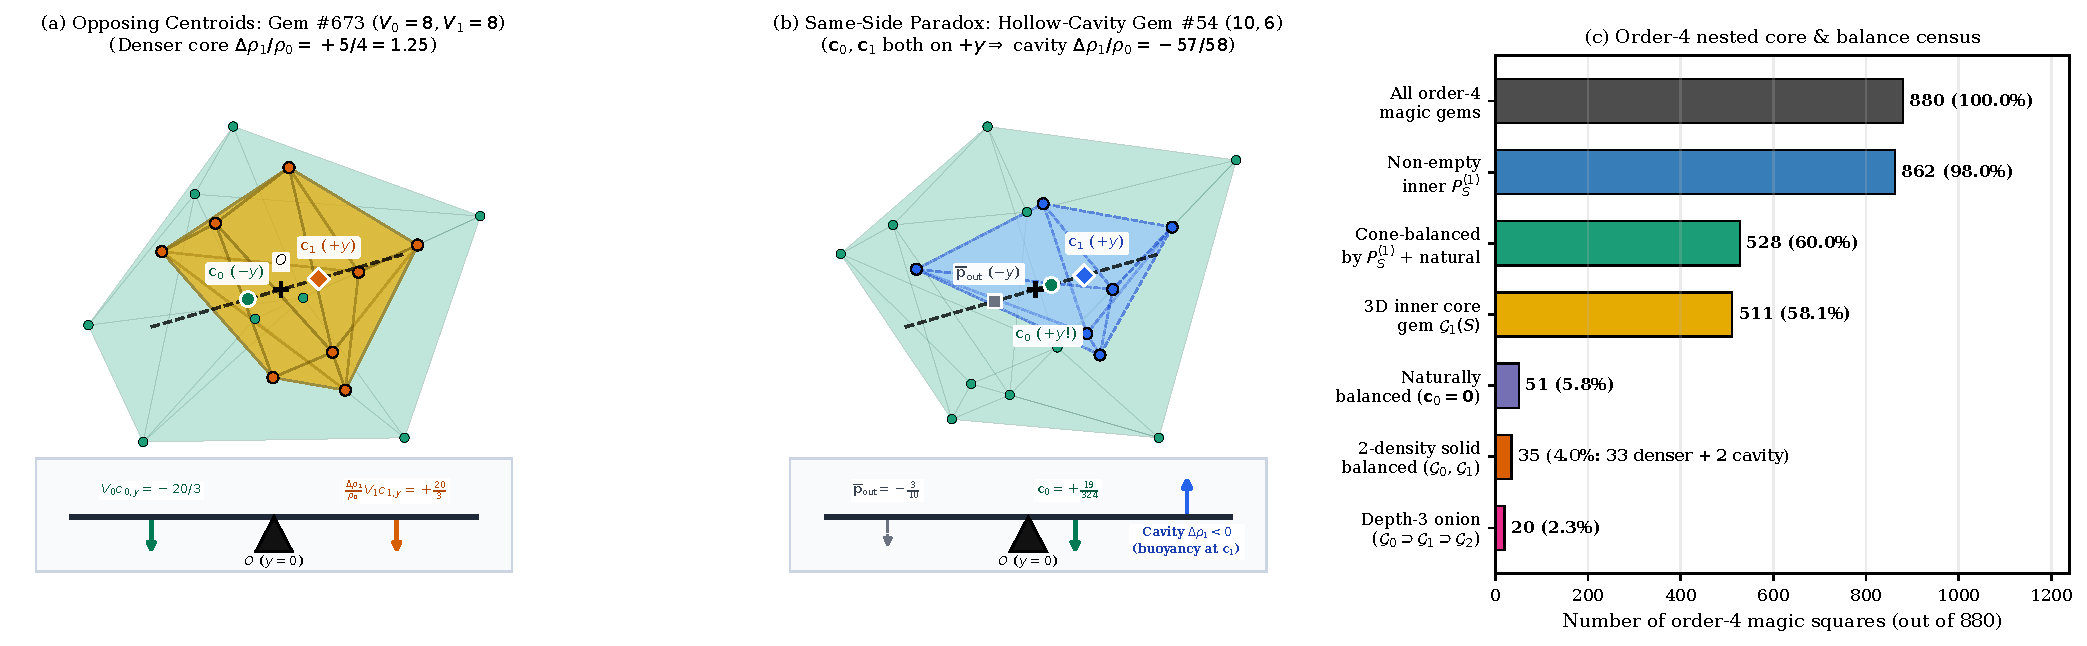
\includegraphics[width=\textwidth]{figures/fig_nested_diamonds.pdf}
\caption{Nested ``diamond-in-a-diamond'' convex layers $\mathcal G_0(S)\supset\mathcal G_1(S)$ and centre-of-mass restoration. (a)~Denser-core Gem \#673 ($(V_0,V_1)=(8,8)$, \Cref{fig:hero-squares}(e)) and (b)~hollow-cavity Gem \#54 ($(V_0,V_1)=(10,6)$, $1$-swap sibling of \#45 in \Cref{fig:hero-squares}(c)), showing the translucent outer hull $\mathcal G_0(S)$ enclosing the inner core gem $\mathcal G_1(S)$ alongside 2D fulcrum lever diagrams at bottom. On \#673, $\mathbf c_0=(0,0,-20/257)$ (green circle) and $\mathbf c_1=(0,0,+2/7)$ (gold diamond) lie on opposite sides of $O$, balancing via a heavier inner core ($\Delta\rho_1/\rho_0=+5/4$, $\rho_1/\rho_0=2.25$). On \#54, although the discrete outer vertices still pull to $-y$ ($\overline{\mathbf p}_{\mathrm{outer}}=(0,-3/10,0)$), volumetric simplex weighting pulls $\mathbf c_0=(0,+19/324,0)$ onto the $+y$ side alongside $\mathbf c_1=(0,+29/68,0)$, so subtracting a $98.3\%$ hollow core cavity ($\Delta\rho_1/\rho_0=-57/58$, $\rho_1/\rho_0=1/58$) restores balance at $O$. (c)~Breakdown of nested layer properties and balance mechanisms across all $880$ order-four magic squares.}
\label{fig:nested-diamonds}
\end{figure}

\subsection{Two-Density Core Inclusions and Inner-Core Weights Restore the Centre of Mass to the Origin}

Guided by \Cref{prop:opposition}, we establish three physical constructions that fabricate a continuous three-dimensional Magic Gem whose centre of mass lies at $O$.

\begin{theorem}[Composite ``diamond-in-a-diamond'' balancing]
\label{thm:diamond-balance}
Let $S$ be an order-four magic square.
\begin{enumerate}
\item \emph{(Two-density solid inclusion $(\mathcal G_0,\mathcal G_1)$.)} Suppose $\dim\mathcal G_1(S)=3$ ($511$ squares), and fabricate $\mathcal G_0(S)$ as a composite solid consisting of a baseline matrix of density $\rho_0>0$ throughout $\mathcal G_0(S)$ together with an inner core inclusion $\mathcal G_1(S)\subset\mathcal G_0(S)$ of excess density $\Delta\rho_1=\rho_1-\rho_0$. The composite centre of mass is
\[
\mathbf c_{\mathrm{comp}} = \frac{\rho_0\vol(\mathcal G_0)\,\mathbf c_0 + \Delta\rho_1\vol(\mathcal G_1)\,\mathbf c_1}{\rho_0\vol(\mathcal G_0) + \Delta\rho_1\vol(\mathcal G_1)}.
\]
Thus $\mathbf c_{\mathrm{comp}}=\mathbf 0$ for some $\Delta\rho_1\ne0$ if and only if $\mathbf c_0$ and $\mathbf c_1$ are non-zero and collinear ($\mathbf c_0\times\mathbf c_1=\mathbf 0$), with unique balancing density increment
\begin{equation}
\label{eq:density-ratio}
\frac{\Delta\rho_1}{\rho_0} = -\frac{\vol(\mathcal G_0)\,(\mathbf c_0\cdot\mathbf c_1)}{\vol(\mathcal G_1)\,\|\mathbf c_1\|_2^2}.
\end{equation}
The $511$ order-four gems with $\dim\mathcal G_1(S)=3$ partition into four exact classes:
\begin{itemize}
\item $207$ gems have $\mathbf c_1=\mathbf 0$ (comprising the $13$ associative gems with $\dim\mathcal G_1=3$ together with $194$ non-associative gems—including \#739 and \#756—whose four inner points form a tetrahedron with vertex sum $\mathbf 0$);
\item $254$ gems (outside Group~VI) have non-collinear solid centroids $\mathbf c_0\times\mathbf c_1\ne\mathbf 0$;
\item $33$ gems (all in Group~VI, where $C_2$ symmetry locks both $\mathbf c_0$ and $\mathbf c_1$ onto the symmetry axis) have strictly anti-parallel solid centroids ($\mathbf c_0\cdot\mathbf c_1<0$), balanced by a \emph{denser} inner core with rational excess density $\Delta\rho_1/\rho_0\in[5/4,\,191/6]$ (\Cref{tab:two-density} and \Cref{tab:all33}); for instance, on Gem \#673 (\Cref{fig:hero-squares}(e), \Cref{fig:nested-diamonds}(a)), eight extreme entries form a U-shaped outer cradle ($V_0=8$, $\overline{\mathbf p}_{\mathrm{outer}}=(0,-1/4,0)$) that swallows the eight intermediate T-core entries ($V_1=8$, $\overline{\mathbf p}_{\mathrm{inner}}=(0,+1/4,0)$), and loading $\mathcal G_1$ to $\Delta\rho_1/\rho_0=5/4$ balances the solid at $O$;
\item $17$ gems (also in Group~VI) have parallel solid centroids pointing in the \emph{same} direction ($\mathbf c_0\cdot\mathbf c_1>0$), because volumetric simplex weighting of $\mathcal G_0(S)\supset\mathcal G_1(S)$ pulls $\mathbf c_0$ to the same side of $O$ as $\mathbf c_1$ despite the opposite discrete vertex centroids of \eqref{eq:opposition}. Balancing these $17$ gems requires $\Delta\rho_1<0$, which is physically realizable with non-negative core density $\rho_1\in[0,\rho_0)$ ($|\Delta\rho_1|/\rho_0\le 1$) for two gems: square \#123 ($\Delta\rho_1/\rho_0=-3/17$, $\rho_1/\rho_0=14/17\approx0.824$, a lighter core) and square \#54 ($\Delta\rho_1/\rho_0=-57/58$, $\rho_1/\rho_0=1/58\approx0.017$, a nearly hollow core cavity, \Cref{fig:nested-diamonds}(b)). Notably, square \#54 is obtained from denser-core square \#45 ($\Delta\rho_1/\rho_0=+85/61$) by swapping a single complementary pair $(8,9)\leftrightarrow(15,2)$ in rows~$2$--$3$ (\Cref{fig:hero-squares}(c)): both have $(V_0,V_1)=(10,6)$, $\overline{\mathbf p}_{\mathrm{outer}}=(0,-3/10,0)$, and $\overline{\mathbf p}_{\mathrm{inner}}=(0,+1/2,0)$, yet inflating the $+y$ hull flares on \#54 pulls $\mathbf c_0$ across $O$ from $(0,-85/856,0)$ to $(0,+19/324,0)$ alongside $\mathbf c_1=(0,+29/68,0)$.
\end{itemize}
\item \emph{(Non-negative inner-core point weighting.)} If $\mathcal G_0(S)$ has uniform density $\rho_0$ and non-negative point masses $m_q\ge0$ are placed at the inner points $q\in P_S^{(1)}$, the composite solid balances at $O$ if and only if $-\mathbf c_0(S)\in\cone(P_S^{(1)})$. This cone condition holds for $477$ of the $829$ unbalanced gems; combined with the $51$ naturally balanced gems, $528$ of the $880$ order-four gems ($60.0\%$) achieve exact balance at $O$ via non-negative inner-core weights.
\item \emph{(Universal barycentric cell / bead-inlaid solid.)} For \emph{every} semi-magic square $S$ of any order $n$, partitioning $\mathcal G_0(S)$ into $N$ cells $C_{ij}$ of equal mass $M/N$ with cell centroids at $\mathbf p_{ij}$ (or embedding $N$ identical dense spherical beads of mass $m_{\mathrm{bead}}$ at $\mathbf p_{ij}$ in a light shell of density $\rho_0\to0$) yields $\mathbf c_{\mathrm{comp}}=\frac1N\sum_{i,j}\mathbf p_{ij}=\mathbf 0$ and restores the exact axisymmetric inertia tensor of \Cref{thm:rotor}.
\end{enumerate}
\end{theorem}

\begin{proof}
Part~(1) follows immediately from setting the first moment $\rho_0\vol(\mathcal G_0)\mathbf c_0+\Delta\rho_1\vol(\mathcal G_1)\mathbf c_1=\mathbf 0$ and evaluating the exact rational simplicial moments (\Cref{sec:appendix}) across all $511$ gems with $\dim\mathcal G_1(S)=3$. In Part~(2), existence of $m_q\ge0$ with $\rho_0\vol(\mathcal G_0)\mathbf c_0+\sum_{q\in P_S^{(1)}}m_q\mathbf p_q=\mathbf 0$ is equivalent to $-\mathbf c_0\in\cone(P_S^{(1)})$, certified by linear programming over the $829$ unbalanced gems. Part~(3) follows from $\sum_{i,j}\mathbf p_{ij}=\mathbf 0$ and \Cref{thm:rotor}.
\end{proof}

\begin{table}[htbp]
\centering
\caption{The eight order-four Magic Gems with the smallest balancing excess density ratios $\Delta\rho_1/\rho_0\in[5/4,40/19]\approx[1.25,2.11]$ in a two-density ``diamond-in-a-diamond'' solid inclusion $(\mathcal G_0(S),\mathcal G_1(S))$ (\Cref{thm:diamond-balance}(1)), all achievable with standard dual-material 3D printing. All $33$ denser-core gems belong to Dudeney's Group~VI, where $C_2$ symmetry forces even vertex counts $(V_0,V_1)$ and aligns $\mathbf c_0$ and $\mathbf c_1$ along the $x$- or $y$-axis. The complete list of $33$ gems is given in \Cref{tab:all33} and \texttt{anc/results\_paper\_c.json}.}
\label{tab:two-density}
\small
\setlength{\tabcolsep}{4.5pt}
\begin{tabular}{r r c c c c c c c}
\toprule
1-idx & 0-idx & $(V_0,V_1)$ & $\vol(\mathcal G_0)$ & $\vol(\mathcal G_1)$ & Axial $c_0$ & Axial $c_1$ & Exact $\Delta\rho_1/\rho_0$ & Decimal $\rho_1/\rho_0$\\
\midrule
\#673 & 672 & $(8,8)$  & $257/3$ & $56/3$ & $-20/257$  & $+2/7$    & $5/4$   & $2.250$\\
\#502 & 501 & $(10,6)$ & $271/3$ & $6$    & $+2/271$   & $-1/12$   & $4/3$   & $2.333$\\
\#45  & 44  & $(10,6)$ & $214/3$ & $6$    & $-85/856$  & $+61/72$  & $85/61$ & $2.393$\\
\#50  & 49  & $(10,6)$ & $254/3$ & $22/3$ & $-7/127$   & $+19/44$  & $28/19$ & $2.474$\\
\#307 & 306 & $(10,6)$ & $277/3$ & $22/3$ & $+23/1108$ & $-15/88$  & $23/15$ & $2.533$\\
\#49  & 48  & $(12,4)$ & $81$    & $2$    & $-2/81$    & $+1/2$    & $2$     & $3.000$\\
\#38  & 37  & $(10,6)$ & $263/3$ & $22/3$ & $+31/1052$ & $-15/88$  & $31/15$ & $3.067$\\
\#47  & 46  & $(10,6)$ & $247/3$ & $22/3$ & $-20/247$  & $+19/44$  & $40/19$ & $3.105$\\
\bottomrule
\end{tabular}
\end{table}

From a practical fabrication standpoint, the $33$ denser-core solids in \Cref{thm:diamond-balance}(1) split into two distinct regimes: the \emph{eight} gems in \Cref{tab:two-density} (\#673, \#502, \#45, \#50, \#307, \#49, \#38, and \#47) require a modest excess density ratio $\Delta\rho_1/\rho_0\in[5/4,\,40/19]\approx[1.25,\,2.11]$ (total core-to-shell density ratio $\rho_1/\rho_0\in[2.25,\,3.11]$), which is directly printable on a dual-extruder 3D printer using standard PLA ($\rho_0\approx1.24\,\mathrm{g/cm^3}$) around a tungsten- or bronze-filled composite filament core ($\rho_1\approx2.8\text{--}4.0\,\mathrm{g/cm^3}$), whereas the remaining $25$ gems in \Cref{tab:all33} have smaller inner-core volumes or shorter lever arms $\|\mathbf c_1\|_2$ and require $\Delta\rho_1/\rho_0\in[47/12,\,191/6]\approx[3.92,\,31.83]$. Overcoming this solid-density barrier—and extending exact balance to the $194$ gems whose tetrahedral core has $\mathbf c_{\mathrm{solid}}(\mathcal G_1)=\mathbf 0$—directly motivates the skeletal and thin-shell architectures of \Cref{subsec:wireframes-nets}: in a nested ball-and-rod wireframe $G(\mathcal G_0)\cup G(\mathcal G_1)$, linear rod mass density scales quadratically with diameter ($\rho_{\mathrm{lin}}\propto d^2$), compressing the required inner-to-outer rod diameter ratio by a square root ($d_1/d_0=\sqrt{\rho_{\mathrm{lin},1}/\rho_{\mathrm{lin},0}}$) and balancing $158$ Group~VI gems using a single homogeneous material.

\subsection{Ball-and-Rod Wireframes, Complete \texorpdfstring{$K_N$}{K\_N} Strut Networks, and Unfolded Papercraft Cutout Nets}
\label{subsec:wireframes-nets}

Beyond solid casting, the companion fabrication suite \cite{mathewson2025magicgemweb} realizes Magic Gems through three skeletal and thin-shell architectures (\Cref{fig:wireframes-nets}):
\begin{enumerate}
\item \emph{Outer and nested ball-and-rod wireframes $G(\mathcal G_0)\cup G(\mathcal G_1)$} (\texttt{magicGem\_v1.stl}), placing spherical or cubic nodes at the lifted points $\mathbf p_u(\lambda)$ and cylindrical rods along the $f_1(\mathcal G_0)$ edges of the outer hull $\mathcal G_0(S)$ and the $f_1(\mathcal G_1)$ edges of the inner core gem $\mathcal G_1(S)$ (\Cref{fig:wireframes-nets}(a));
\item \emph{Fully interconnected complete strut networks $K_N\bigl(P_S(\lambda)\bigr)$} (\texttt{magicGem\_v2.stl}), connecting all $\binom{N}{2}$ pairs of lifted points $\mathbf p_u(\lambda),\mathbf p_v(\lambda)$ ($120$ rods at $n=4$: $f_1(\mathcal G_0)$ outer boundary edges plus $120-f_1(\mathcal G_0)$ internal cross-struts running through the interior of the hull, \Cref{fig:wireframes-nets}(b)); and
\item \emph{Unfolded 2D papercraft cutout nets with trapezoidal glue tabs}, unfolding the boundary surface $\partial\mathcal G_\lambda(S)$ into a flat printable net along a breadth-first spanning tree of the dual facet graph $G^*(\mathcal G)$ (\Cref{fig:wireframes-nets}(c)).
\end{enumerate}

\begin{theorem}[Universal covariance of the complete $K_N$ strut network versus length-weighted and nested wireframes]
\label{thm:complete-network}
Let $S$ be an arrangement of $\{1,\dots,N\}$, $N=n^2$ ($n\ge2$), with lifted point cloud $P_S(\lambda)=\{\mathbf p_1(\lambda),\dots,\mathbf p_N(\lambda)\}\subset\R^3$ satisfying $\sum_{u=1}^N\mathbf p_u(\lambda)=\mathbf 0$ and empirical covariance matrix $\Sigma(\lambda)=\frac1N\sum_{u=1}^N\mathbf p_u(\lambda)\mathbf p_u(\lambda)^{\top}$. In the one-dimensional slender-rod (line-skeleton) limit $d/L_{uv}\to 0^+$, where each rod is concentrated along its centreline segment:
\begin{enumerate}
\item \emph{(Equal-mass-per-edge complete network $K_N$.)} Suppose each of the $\binom{N}{2}$ slender rods connecting $\mathbf p_u(\lambda)$ and $\mathbf p_v(\lambda)$ ($1\le u<v\le N$) carries equal mass $m_{\mathrm{edge}}=M_{\mathrm{rods}}/\binom{N}{2}$ (together with optional equal node masses $m_{\mathrm{node}}=M_{\mathrm{nodes}}/N$ at the $N$ vertices, where $M_{\mathrm{nodes}}=\theta M$ and $M_{\mathrm{rods}}=(1-\theta)M$ for $\theta\in[0,1]$). Because $K_N$ is $(N-1)$-regular, the centre of mass of $K_N\bigl(P_S(\lambda)\bigr)$ lies at the origin $O$ for \emph{every} arrangement $S$:
\begin{equation}
\label{eq:kN-com}
\mathbf c\bigl(K_N(\lambda)\bigr) = \frac{1}{\binom{N}{2}}\sum_{1\le u<v\le N}\frac{\mathbf p_u(\lambda)+\mathbf p_v(\lambda)}{2} = \frac{1}{N}\sum_{u=1}^N\mathbf p_u(\lambda) = \mathbf 0.
\end{equation}
Furthermore, the continuous second-moment covariance matrix of the $\binom{N}{2}$ equal-mass slender rods is an exact universal scalar multiple of the discrete covariance matrix $\Sigma(\lambda)$:
\begin{equation}
\label{eq:kN-cov}
\Sigma_{\mathrm{rods}}^{(=\text{mass})}\bigl(K_N(\lambda)\bigr)
= \frac{2N-3}{3(N-1)}\,\Sigma(\lambda)
\qquad\Bigl(=\frac{5}{8}\,\Sigma(\lambda)\text{ at }n=3,\quad \frac{29}{45}\,\Sigma(\lambda)\text{ at }n=4\Bigr).
\end{equation}
Consequently, for \emph{every} semi-magic square $S$ of order $n$ and every node-mass fraction $\theta\in[0,1]$, the composite complete network $K_N\bigl(P_S(\lambda)\bigr)$ has covariance $\bigl(\theta+(1-\theta)\frac{2N-3}{3(N-1)}\bigr)\Sigma(\lambda)$ and therefore shares the \emph{exact same axisymmetric inertia ratio $I_\perp(\lambda)/I_{zz}=\frac12\bigl(1+\lambda^2(n^2+1)\bigr)$, the exact same spherical-top scale $\lambda_{\mathrm{iso}}=(n^2+1)^{-1/2}$, and the exact same integer polhode ratio $(n^2+2)/2=9$ at $\lambda=1$} as the discrete point cloud in \Cref{thm:rotor}.
\item \emph{(Length-weighted strut networks $\rho_{\mathrm{lin}}=\mathrm{const}$.)} When a subgraph $G=(V_G,E_G)$ is fabricated from slender rods of uniform cross-sectional diameter $d$ and linear mass density $\rho_{\mathrm{lin}}=\frac\pi4 d^2\rho_{\mathrm{mat}}$, each rod $(u,v)\in E_G$ has mass proportional to its Euclidean length $L_{uv}(\lambda)=\|\mathbf p_u(\lambda)-\mathbf p_v(\lambda)\|_2$, total rod length $L(G;\lambda)=\sum_{(u,v)\in E_G}L_{uv}(\lambda)$, and length-weighted centroid
\[
\mathbf c_{\mathrm{len}}(G;\lambda) = \frac{1}{2L(G;\lambda)}\sum_{u\in V_G}\Biggl(\sum_{v:\,(u,v)\in E_G}L_{uv}(\lambda)\Biggr)\mathbf p_u(\lambda).
\]
Across all $880$ order-four magic squares (\Cref{fig:wireframes-nets}(d)):
\begin{itemize}
\item Both the $120$-rod complete network $K_{16}$ and the outer hull wireframe $G(\mathcal G_0)$ have $\mathbf c_{\mathrm{len}}=\mathbf 0$ if and only if $S$ is one of the $48$ centrally symmetric associative squares ($5.5\%$).
\item Passing from the outer hull wireframe $G(\mathcal G_0)$ (mean total rod length $\overline L=143.30$ at $\lambda=1$ and $60.00$ at $\lambda=0.20$) to the complete $120$-rod network $K_{16}$ ($\overline L=756.14$ at $\lambda=1$ and $305.34$ at $\lambda=0.20$) reduces the mean centroid drift $\|\mathbf c_{\mathrm{len}}\|_2$ by $2.7\times$ at $\lambda=1$ (from $0.1940$ to $0.0717$) and by $3.6\times$ at $\lambda=0.20$ (from $0.0879$ to $0.0247$, versus $0.0888$ for the uniform solid), while tightening the mean transverse inertia splitting $(I_3-I_2)/I_2$ to $0.0051$ at $\lambda=1$.
\end{itemize}
\item \emph{(Composite balance of nested wireframes $G(\mathcal G_0)\cup G(\mathcal G_1)$ via rod diameter tuning.)} For the $848$ order-four gems with $\dim\mathcal G_1(S)\ge1$, fabricating the outer edges $E(\mathcal G_0)$ with rod diameter $d_0$ and the disjoint inner core edges $E(\mathcal G_1)$ with rod diameter $d_1$ yields $\mathbf c_{\mathrm{wire}}(\mathcal G_0\cup\mathcal G_1)=\mathbf 0$ whenever $\mathbf c_{\mathrm{wire}}(\mathcal G_0)$ and $\mathbf c_{\mathrm{wire}}(\mathcal G_1)$ are strictly anti-parallel, at the unique rod diameter ratio
\begin{equation}
\label{eq:rod-diam-ratio}
\frac{d_1}{d_0} = \sqrt{\frac{\rho_{\mathrm{lin},1}}{\rho_{\mathrm{lin},0}}}
= \sqrt{-\frac{L\bigl(G(\mathcal G_0)\bigr)\,\bigl(\mathbf c_{\mathrm{wire}}(\mathcal G_0)\cdot\mathbf c_{\mathrm{wire}}(\mathcal G_1)\bigr)}{L\bigl(G(\mathcal G_1)\bigr)\,\|\mathbf c_{\mathrm{wire}}(\mathcal G_1)\|_2^2}}.
\end{equation}
Because $E(\mathcal G_0)\cap E(\mathcal G_1)=\emptyset$, any ratio $d_1/d_0>0$ is physically realizable without cavity constraints. Consequently, exact composite wireframe balance holds for $158$ Group~VI gems at $\lambda=1$ ($81$ with $\dim\mathcal G_1=3$, $37$ with $\dim\mathcal G_1=2$, $40$ with $\dim\mathcal G_1=1$; e.g., Gem \#673 at $d_1/d_0=0.7932$ and Gem \#45 at $d_1/d_0=0.7945$) and for $164$ Group~VI gems at $\lambda=0.20$ ($83$ with $\dim\mathcal G_1=3$; e.g., Gem \#673 at $d_1/d_0=0.4932$ and Gem \#45 at $d_1/d_0=0.7694$).
\end{enumerate}
\end{theorem}

\begin{proof}
(1) Integrating $\mathbf x(t)=(1-t)\mathbf p_u+t\mathbf p_v$ over $t\in[0,1]$ gives the rod midpoint $\frac12(\mathbf p_u+\mathbf p_v)$ and second-moment matrix
\[
M_2(u,v) = \int_0^1 \mathbf x(t)\mathbf x(t)^{\top}\,dt = \frac{1}{3}\bigl(\mathbf p_u\mathbf p_u^{\top} + \mathbf p_v\mathbf p_v^{\top}\bigr) + \frac{1}{6}\bigl(\mathbf p_u\mathbf p_v^{\top} + \mathbf p_v\mathbf p_u^{\top}\bigr).
\]
In $K_N$, each vertex $u$ belongs to $N-1$ edges, proving \eqref{eq:kN-com} and giving $\sum_{u<v}(\mathbf p_u\mathbf p_u^{\top}+\mathbf p_v\mathbf p_v^{\top})=(N-1)\sum_{u=1}^N\mathbf p_u\mathbf p_u^{\top}=N(N-1)\Sigma(\lambda)$. Similarly, expanding $\mathbf 0=\bigl(\sum_u\mathbf p_u\bigr)\bigl(\sum_v\mathbf p_v\bigr)^{\top}$ yields $\sum_{u<v}(\mathbf p_u\mathbf p_v^{\top}+\mathbf p_v\mathbf p_u^{\top})=-\sum_{u=1}^N\mathbf p_u\mathbf p_u^{\top}=-N\Sigma(\lambda)$. Dividing by $\binom{N}{2}=\frac12N(N-1)$ gives
\[
\Sigma_{\mathrm{rods}}^{(=\text{mass})}\bigl(K_N(\lambda)\bigr)
= \frac{2}{N(N-1)}\left(\frac{N-1}{3} - \frac{1}{6}\right)N\Sigma(\lambda)
= \frac{2N-3}{3(N-1)}\,\Sigma(\lambda),
\]
establishing \eqref{eq:kN-cov}. Parts~(2) and~(3) follow by evaluating $L(G;\lambda)$, $\mathbf c_{\mathrm{len}}(G;\lambda)$, and \eqref{eq:rod-diam-ratio} across all $880$ squares (\Cref{sec:appendix}).
\end{proof}

\begin{proposition}[Papercraft cutout nets, topological glue-tab invariant, and thin-shell balance]
\label{prop:papercraft-net}
Let $\mathcal G_\lambda(S)$ be any three-dimensional Magic Gem with $f$-vector $(f_0,f_1,f_2)$.
\begin{enumerate}
\item \emph{(Universal glue-tab invariant $N_{\mathrm{tabs}}=f_0-1$ and non-overlapping order-four nets.)} Unfolding $\partial\mathcal G_\lambda(S)$ into a connected planar cutout net along any spanning tree $T^*$ of the dual facet graph $G^*(\mathcal G)$ \cite{durer1525underweysung,shephard1975convex,demaine2007geometric,ghomi2014durer} partitions the $f_1$ polyhedral edges into $|E_{\mathrm{fold}}|=f_2-1$ interior fold lines (dashed creases in \Cref{fig:wireframes-nets}(c)) and $N_{\mathrm{tabs}}=f_1-(f_2-1)$ cut edges, each opened into a pair of exterior boundary segments joined by one trapezoidal glue tab (labelled in matching pairs \texttt{a}--\texttt{k} in \Cref{fig:wireframes-nets}(c)). Because $\partial\mathcal G_\lambda(S)\cong S^2$ is a genus-$0$ planar surface, the cut edges $E\setminus E(T^*)$ form a complementary spanning tree $T$ of the primal $1$-skeleton $G(\mathcal G_\lambda)$ on the $f_0$ hull vertices (equivalently, the cycle rank $\beta_1(G^*)=f_1-f_2+1$ of the dual graph equals $f_0-1$ by Euler's formula $f_0-f_1+f_2=2$), so the number of glue tabs depends \emph{solely on the hull vertex count $f_0$}:
\begin{equation}
\label{eq:glue-tabs}
N_{\mathrm{tabs}} = f_1 - (f_2 - 1) = |E(T)| = f_0 - 1,
\end{equation}
and the net perimeter consists of $2(f_0-1)$ cut boundary segments. Moreover, \eqref{eq:glue-tabs} is strictly invariant under triangulating non-triangular facets into $F_\Delta=2f_0-4$ triangles and $E_\Delta=3f_0-6$ edges, since $E_\Delta-(F_\Delta-1)=(3f_0-6)-(2f_0-5)=f_0-1$. Across the $880$ order-four Magic Gems, $N_{\mathrm{tabs}}=f_0-1$ takes every integer value in $\{7,\dots,15\}$ (distributed as $7$ gems with $7$ tabs, $10$ with $8$, $103$ with $9$, $80$ with $10$, $380$ with $11$ including D\"urer's gem \#175, $106$ with $12$, $162$ with $13$, $14$ with $14$, and $18$ with $15$ tabs). Under the deterministic breadth-first dual spanning tree $T^*$ rooted at the largest-area facet $F_0$ (marked $\bigstar F_0$ in \Cref{fig:wireframes-nets}(c), visiting adjacent facets in canonical index order), \emph{all $880$ order-four Magic Gems ($100\%$) unfold into strictly non-overlapping 2D planar nets} at both $\lambda=1$ and $\lambda=0.20$.
\item \emph{(Hollow thin-shell mechanics $\partial\mathcal G_\lambda(S)$ and nested shell balance.)} In the idealized mathematical shell model $\partial\mathcal G_\lambda(S)$ of uniform areal mass density $\sigma_0>0$ (with massless glue tabs, or butt-jointed laser-cut facets), the surface area is $\operatorname{area}(\partial\mathcal G_\lambda)\in[116.53,148.62]$ (mean $135.13$) at $\lambda=1$ and $[31.26,40.02]$ (mean $36.38$) at $\lambda=0.20$, with area-weighted centroid $\mathbf c_{\mathrm{shell}}(\mathcal G_0)=\frac{1}{\operatorname{area}(\partial\mathcal G_0)}\sum_F A_F\mathbf c(F)$ vanishing on all $48$ associative squares and having mean drift $0.1357$ at $\lambda=1$ ($0.0907$ at $\lambda=0.20$). Enclosing a nested inner shell $\partial\mathcal G_1(S)$ ($\dim\mathcal G_1=3$) of areal density $\sigma_1$ restores exact composite balance $\mathbf c_{\mathrm{shell}}(\partial\mathcal G_0\cup\partial\mathcal G_1)=\mathbf 0$ for $80$ Group~VI gems at $\lambda=1$ and $87$ Group~VI gems at $\lambda=0.20$ (including Gem \#673 at $\sigma_1/\sigma_0=0.9110$ for $\lambda=1$ and $0.6826$ for $\lambda=0.20$, and Gem \#45 at $\sigma_1/\sigma_0=0.0849$ for $\lambda=1$ and $0.2003$ for $\lambda=0.20$).
\end{enumerate}
\end{proposition}

\begin{proof}
By planar graph duality on $\partial\mathcal G_\lambda(S)\cong S^2$, the complement of a dual spanning tree $T^*\subset G^*(\mathcal G_\lambda)$ ($|E(T^*)|=f_2-1$) is a primal spanning tree $T\subset G(\mathcal G_\lambda)$ on the $f_0$ vertices, giving $N_{\mathrm{tabs}}=|E(T)|=f_0-1$ directly (and matching $f_1-(f_2-1)=f_0-1$ by Euler's formula). Whether every convex polyhedron admits a non-overlapping edge unfolding remains open in general (D\"urer's conjecture \cite{durer1525underweysung,shephard1975convex,demaine2007geometric,ghomi2014durer}); for the $880$ order-four Magic Gems at $\lambda=1$ and $\lambda=0.20$, exact 2D polygon intersection testing of the breadth-first dual spanning-tree unfolding and exact triangular surface moments certify non-overlap and the stated shell censuses across all $880$ gems (\Cref{sec:appendix}).
\end{proof}

\begin{remark}[Finite-diameter cylinders, hub intersections, and core suspension]
\label{rem:finite-diameter}
In a physical 3D print of finite rod diameter $d>0$, each right circular cylinder of length $L_{uv}$ and unit direction $\hat{\mathbf e}_{uv}=(\mathbf p_v-\mathbf p_u)/L_{uv}$ has midpoint centroid $\frac12(\mathbf p_u+\mathbf p_v)$ (leaving \eqref{eq:kN-com} unchanged) and adds the transverse radial inertia correction $m_{uv}\frac{d^2}{16}(I_3+\hat{\mathbf e}_{uv}\hat{\mathbf e}_{uv}^{\top})$ to its slender-rod inertia tensor, while boolean union at the $16$ degree-$15$ vertex hubs and interior strut crossings subtracts $O(d^3)$ cap-overlap volumes. To suspend the disjoint inner core wireframe $G(\mathcal G_1)$ inside $G(\mathcal G_0)$ on a Group~VI gem, one connects them by either lightweight tension filaments or $C_2$-symmetric pairs of equal-length struts whose midpoint centroid lies at $O$, leaving the balancing diameter ratio $d_1/d_0$ in \eqref{eq:rod-diam-ratio} invariant. Finally, the jump from $35$ two-density balanced solids (\Cref{thm:diamond-balance}(1)) to $158$ balanced nested wireframes at $\lambda=1$ arises because $194$ non-associative gems have a $4$-vertex tetrahedral core $\mathcal G_1(S)$ with $\sum_{q\in P_S^{(1)}}\mathbf p_q=\mathbf 0$: its solid centroid is $\mathbf c_{\mathrm{solid}}(\mathcal G_1)=\frac14\sum\mathbf p_q=\mathbf 0$, which cannot counter $\mathbf c_0\ne\mathbf 0$, whereas its six edges have unequal Euclidean lengths on opposite sides of $O$, producing a non-zero wireframe centroid $\mathbf c_{\mathrm{wire}}(\mathcal G_1)\ne\mathbf 0$ along the Group~VI $C_2$ axis.
\end{remark}

\begin{figure}[htbp]
\centering
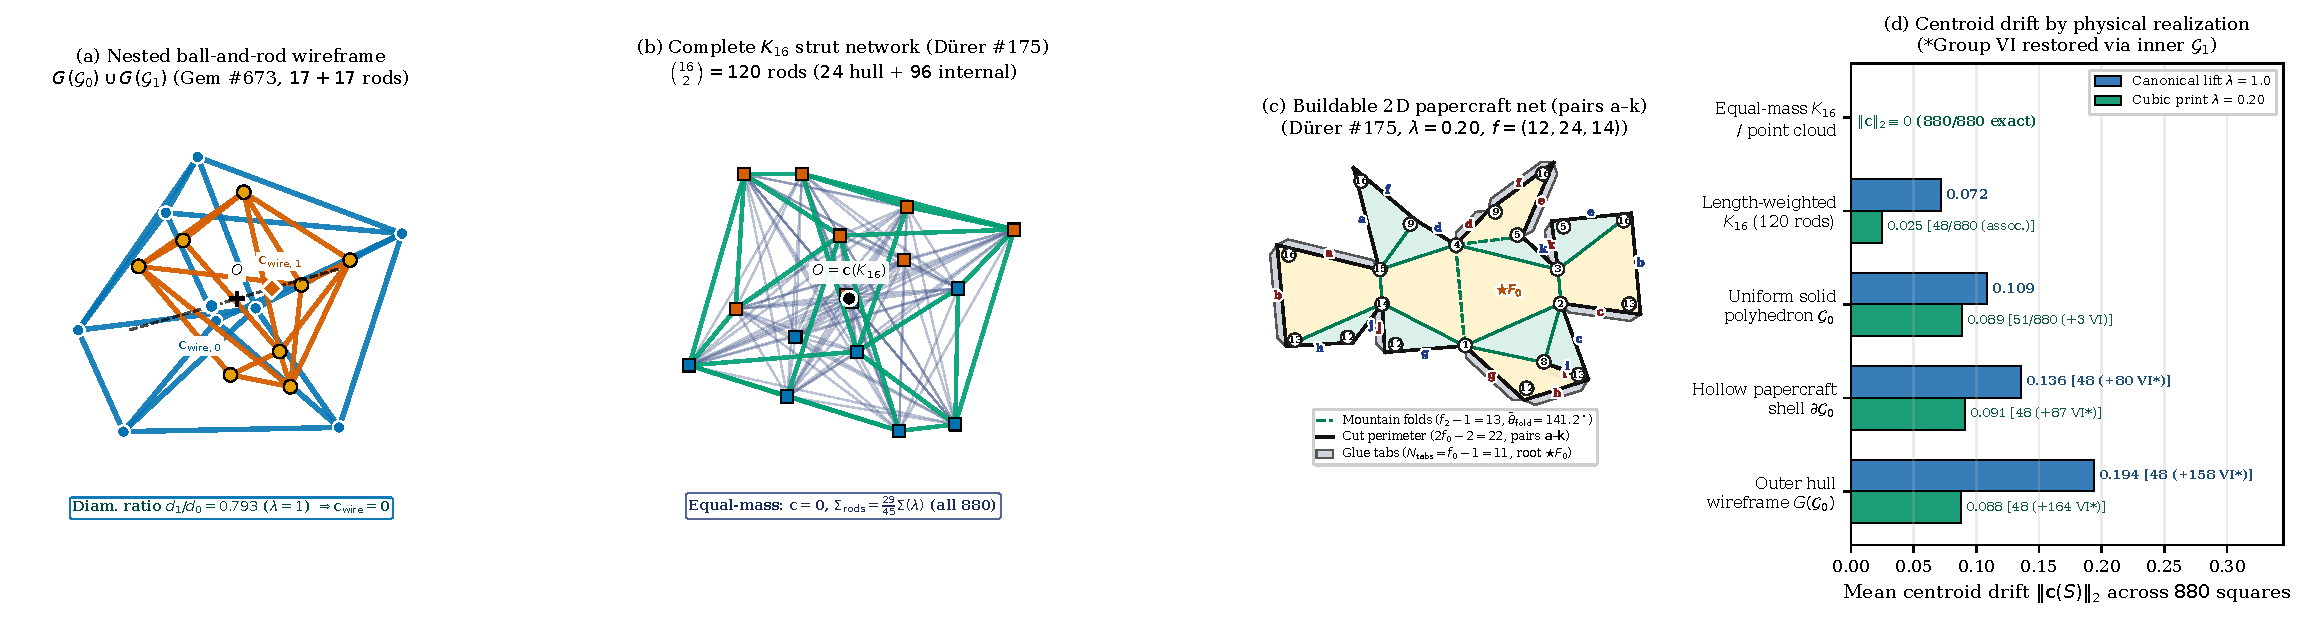
\includegraphics[width=\textwidth]{figures/fig_wireframes_and_nets.pdf}
\caption{Wireframes, complete $K_{16}$ strut networks, and unfolded papercraft cutout nets of Magic Gems \cite{mathewson2025magicgemweb}. (a)~Nested ball-and-rod wireframe $G(\mathcal G_0)\cup G(\mathcal G_1)$ of Gem \#673 ($17$ outer blue rods + $17$ inner orange rods), where tuning the inner-to-outer rod diameter ratio to $d_1/d_0=0.793$ at $\lambda=1$ ($0.493$ at $\lambda=0.20$) restores $\mathbf c_{\mathrm{wire}}=\mathbf 0$. (b)~Fully interconnected complete network $K_{16}$ of D\"urer's Gem \#175 (\texttt{magicGem\_v2.stl}) with all $\binom{16}{2}=120$ rods ($24$ outer hull edges in green + $96$ internal cross-struts in slate) and $16$ node cubes; for equal-mass rods, $\mathbf c(K_{16})=\mathbf 0$ and $\Sigma_{\mathrm{rods}}=\frac{29}{45}\Sigma(\lambda)$ for all $880$ squares (\Cref{thm:complete-network}(1)). (c)~Exact 2D unfolded papercraft cutout net of D\"urer's Gem \#175 ($\lambda=0.20$, $f=(12,24,14)$) rooted at $\bigstar F_0$, with $f_2-1=13$ dashed fold lines (mean dihedral fold angle $\overline{\theta}_{\mathrm{fold}}=141.2^\circ\in[117^\circ,165^\circ]$), $2f_0-2=22$ solid cut perimeter segments, $N_{\mathrm{tabs}}=f_0-1=11$ grey trapezoidal glue tabs paired with their mating cut edges by lowercase labels \texttt{a}--\texttt{k} (\Cref{prop:papercraft-net}(1)), and magic entries $s_{ij}$ at the unfolded vertices. (d)~Comparison of mean centroid drift $\|\mathbf c(S)\|_2$ across all $880$ order-four magic squares for the five physical realizations at $\lambda=1.0$ and $\lambda=0.20$.}
\label{fig:wireframes-nets}
\end{figure}


\section{Mirror-Twin Inversion Locks Gems into Vertical Towers}
\label{sec:stacking}

Our final mechanical investigation treats Magic Gems as physical building blocks under gravity. When a polyhedron $\mathcal G_\lambda(S)$ rests on a flat horizontal table on one of its facets $F$, or when multiple gems are stacked face-to-face into a vertical column, two geometric questions arise: (i)~when is a resting facet statically stable against tipping under gravity, and (ii)~how can copies of a gem be stacked along slanted facets without the column curving away from the vertical and toppling?

\subsection{Cubic Aspect Scaling Raises Facet Resting Stability from \texorpdfstring{$43.0\%$}{43.0\%} to \texorpdfstring{$74.5\%$}{74.5\%}}

Let $F\subset\partial\mathcal G_\lambda(S)$ be a facet with outward unit normal $\hat{\mathbf n}_F(\lambda)$. When $\mathcal G_\lambda(S)$ rests with $F$ on a horizontal plane (so $\hat{\mathbf n}_F(\lambda)$ points straight down), gravity acts vertically through the centre of mass $\mathbf c(\lambda)$. Let $\pi_F(\mathbf c(\lambda))$ denote the orthogonal projection of $\mathbf c(\lambda)$ onto the affine plane of $F$, and let $h_F(\lambda)=(\mathbf p_F-\mathbf c(\lambda))\cdot(-\hat{\mathbf n}_F(\lambda))>0$ be the height of the centre of mass above the table.

\begin{definition}[Static stability margin and critical tipping angle]
\label{def:stability}
For a facet $F\subset\partial\mathcal G_\lambda(S)$, the \emph{stability margin} $d_{\mathrm{stab}}(S,F;\lambda)$ is the signed Euclidean distance in the plane of $F$ from $\pi_F(\mathbf c(\lambda))$ to the boundary $\partial F$ of the facet polygon (taken positive when $\pi_F(\mathbf c(\lambda))$ lies in the strict relative interior of $F$, and negative outside). Facet $F$ is \emph{statically stable} if and only if $d_{\mathrm{stab}}(S,F;\lambda)>0$, in which case its \emph{critical tipping angle} (the maximum tilt of the table before $\mathcal G_\lambda(S)$ topples across an edge of $F$) is
\begin{equation}
\label{eq:tip-angle}
\theta_{\mathrm{tip}}(S,F;\lambda) = \arctan\!\left(\frac{d_{\mathrm{stab}}(S,F;\lambda)}{h_F(\lambda)}\right).
\end{equation}
\end{definition}

\begin{proposition}[Order-four resting stability census]
\label{prop:stability-census}
Across all $880$ magic squares of order~$4$, the gems $\mathcal G_\lambda(S)$ possess a total of $14{,}824$ facets (mean $16.85$ facets per gem).
\begin{enumerate}
\item At the canonical lift $\lambda=1$, using the exact uniform-solid centre of mass $\mathbf c_0(S)$, exactly $6{,}378$ of the $14{,}824$ facets ($43.0\%$) are statically stable, with every gem possessing between $4$ and $12$ stable resting facets (mean $7.25$; using the balanced point centroid $O$ gives $6{,}340$ stable facets, $42.8\%$).
\item At the cubic 3D-print scale $\lambda_{\mathrm{cube}}=1/5=0.20$ (where the height span of $1,\dots,16$ equals the $3\times3$ grid footprint), the reduced vertical aspect ratio brings the centre of mass closer to the slanted upper and lower facets: $11{,}044$ of the $14{,}824$ facets ($74.5\%$) are statically stable, with a mean critical tipping angle of $17.8^\circ$ and a maximum of $47.3^\circ$ (\Cref{fig:mirror-stacking}(d)).
\end{enumerate}
\end{proposition}

\begin{proof}
For each of the $880$ gems and each facet $F\subset\partial\mathcal G_\lambda(S)$ with exact integer plane equation $aX+bY+cZ+d=0$ in doubled coordinates, rescaling $z\mapsto\lambda z$ transforms the outward normal to $\mathbf n_F(\lambda)\propto(a\lambda,b\lambda,c)$ and the solid centroid to $\mathbf c_0(\lambda)=(c_{0,x},c_{0,y},\lambda c_{0,z})$. Projecting $\mathbf c_0(\lambda)$ onto an orthonormal basis of the affine plane of $F$ and evaluating the signed edge distances $d_{\mathrm{stab}}(S,F;\lambda)$ and \eqref{eq:tip-angle} across all $14{,}824$ facets at $\lambda=1$ and $\lambda=0.20$ yields the stated counts and extremal angles.
\end{proof}

\subsection{Central Inversion Pairs Every Upper Facet with a Parallel Lower Facet of Its Mirror Twin}

Suppose we wish to stack multiple blocks vertically along an upper facet $F_+\subset\mathcal G_\lambda(S)$ (with outward normal $\mathbf n_+$, $n_{+,z}>0$) and a lower facet $F_-\subset\mathcal G_\lambda(S)$ (with outward normal $\mathbf n_-$, $n_{-,z}<0$). Stacking translated copies of the \emph{same} gem $\mathcal G_\lambda(S)$ without rotation requires $\mathbf n_-=-\mathbf n_+$ (which holds for only $124$ of the $880$ gems); when $\mathbf n_-\ne-\mathbf n_+$, same-gem copies meet at an open wedge gap (\Cref{fig:mirror-stacking}(c), left). Pairing a gem with its \emph{rotational complement (mirror twin)}
\begin{equation}
\label{eq:mirror-twin}
S^* := r^2\overline S = (N+1)\mathbf 1 - r^2 S
\end{equation}
solves the stacking problem universally via central inversion in $\R^3$ (\Cref{fig:mirror-stacking}(a,c)).

\begin{figure}[htbp]
\centering
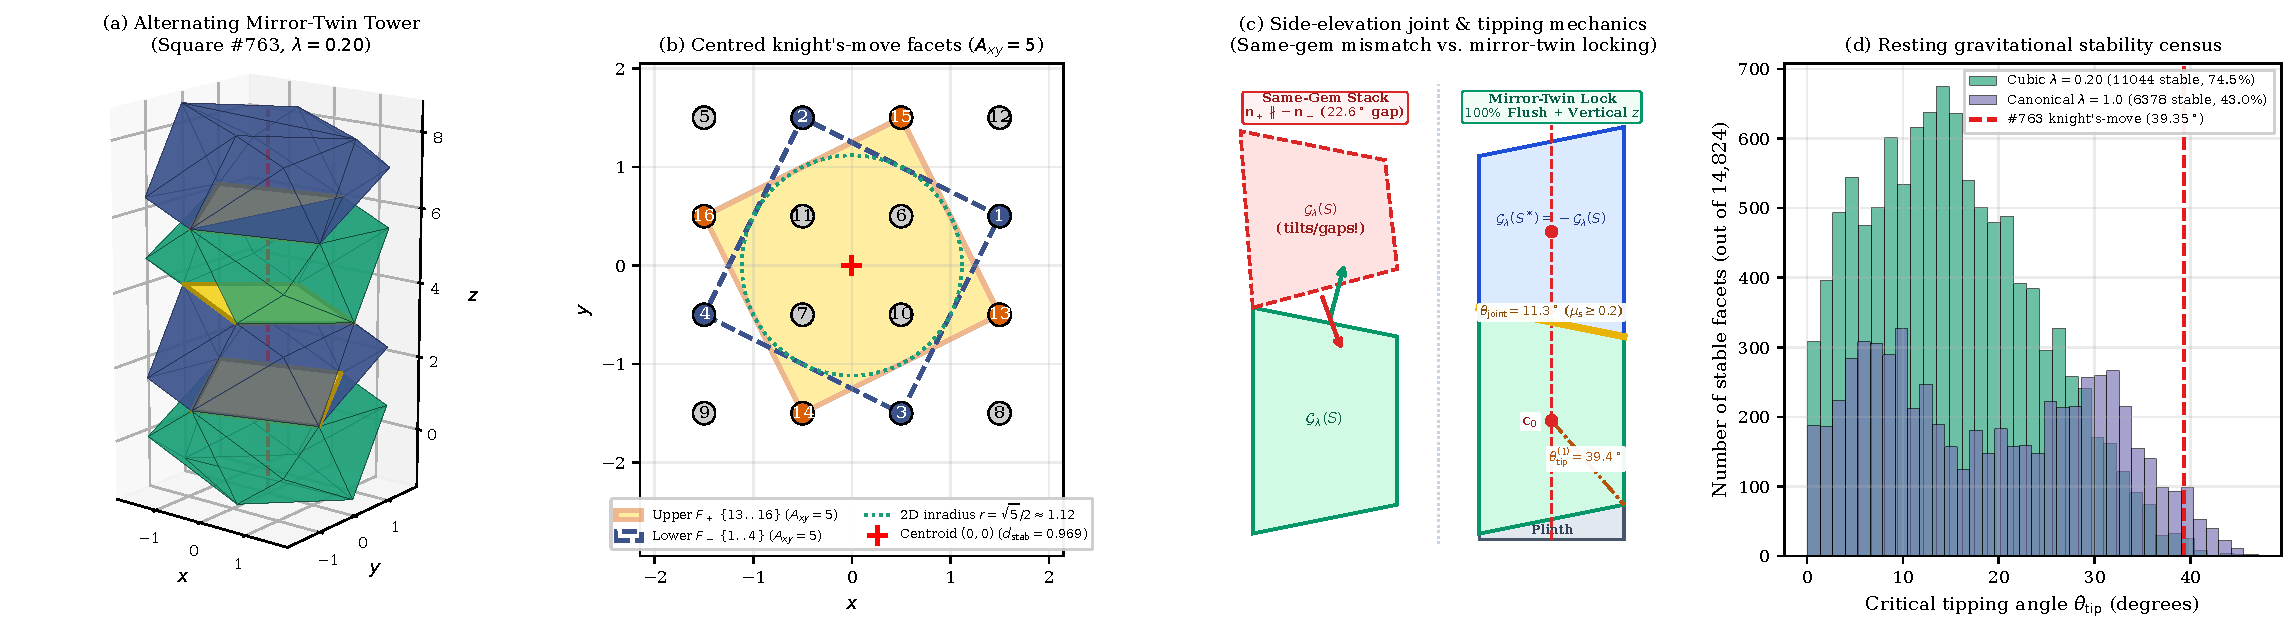
\includegraphics[width=\textwidth]{figures/fig_mirror_stacking.pdf}
\caption{Mirror-twin facet locking and periodic vertical towers. (a)~Four-block alternating tower of square \#763 at the cubic 3D-print scale $\lambda=0.20$, alternating $\mathcal G_\lambda(S)$ (green) with its mirror twin $\mathcal G_\lambda(r^2\overline S)=-\mathcal G_\lambda(S)$ (blue); the golden contact joints are the centred knight's-move squares $\{13,14,15,16\}$ and $\{1,2,3,4\}$, which meet with $100\%$ vertex congruence and keep the column's centre of mass on the vertical $z$-axis (red dashed). (b)~Top-down $(x,y)$ footprint of square \#763 showing the dual knight's-move squares of area $A_{xy}=5$ and 2D footprint inradius $r=\sqrt{5}/2\approx1.12$ (while the 3D tilted-plane stability margin from $\mathbf c_0$ is $d_{\mathrm{stab}}=0.969$ at $\lambda=0.20$). (c)~Two-dimensional side-elevation joint and tipping schematic comparing the $2\theta_{\mathrm{joint}}=22.6^\circ$ wedge mismatch of unrotated same-gem stacking against flush mirror-twin locking ($\mathbf n_+^*=-\mathbf n_+$) on a $\theta_{\mathrm{joint}}=11.3^\circ$ base plinth. (d)~Census of critical tipping angles $\theta_{\mathrm{tip}}$ over all $14{,}824$ facets at $\lambda=0.20$ and $\lambda=1.0$.}
\label{fig:mirror-stacking}
\end{figure}

\begin{theorem}[Mirror-Twin Inversion and Zero-Rotation Alternating Towers]
\label{thm:mirror-tower}
Let $S$ be any arrangement of order $n$, let $S^*=r^2\overline S$ be its half-turned complement, and let $\lambda>0$.
\begin{enumerate}
\item \emph{(Central inversion identity.)} In $\R^3$, the lifted point clouds and convex hulls satisfy
\begin{equation}
\label{eq:central-inv}
P_{S^*}(\lambda) = -P_S(\lambda),\qquad
\mathcal G_\lambda(S^*) = -\mathcal G_\lambda(S).
\end{equation}
Consequently, the map $F\mapsto F^*:=-F$ is an area-preserving, normal-reversing bijection between the upper facets $F_+\subset\mathcal G_\lambda(S)$ (outward normal $+\mathbf n_+$) and the lower facets $F_+^*\subset\mathcal G_\lambda(S^*)$ (outward normal $-\mathbf n_+$), and between the lower facets $F_-\subset\mathcal G_\lambda(S)$ (outward normal $+\mathbf n_-$) and the upper facets $F_-^*=-F_-\subset\mathcal G_\lambda(S^*)$ (outward normal $-\mathbf n_-$).
\item \emph{(Zero-rotation alternating tower.)} Choose \emph{any} upper facet $F_+\subset\mathcal G_\lambda(S)$ and \emph{any} lower facet $F_-\subset\mathcal G_\lambda(S)$ (not necessarily parallel) that are centrally symmetric polygons in $\R^3$ with centroids $\mathbf c(F_+)$ and $\mathbf c(F_-)$. Define the alternating sequence of unrotated blocks $B_0,B_1,B_2,\dots$ by
\begin{equation}
\label{eq:tower-blocks}
B_{2m} = \mathcal G_\lambda(S) + m\mathbf T,\qquad
B_{2m+1} = -\mathcal G_\lambda(S) + 2\mathbf c(F_+) + m\mathbf T,\qquad
\mathbf T = 2\bigl(\mathbf c(F_+) - \mathbf c(F_-)\bigr).
\end{equation}
Then:
\begin{enumerate}
\item At every odd joint $B_{2m}\cap B_{2m+1}$, the upper facet $F_+ + m\mathbf T$ of $B_{2m}$ coincides \emph{identically} (100\% polygon and vertex overlap, with opposite outward normals $\pm\mathbf n_+$) with the lower facet $-F_+ + 2\mathbf c(F_+) + m\mathbf T$ of $B_{2m+1}$.
\item At every even joint $B_{2m-1}\cap B_{2m}$, the upper facet $-F_- + 2\mathbf c(F_+) + (m-1)\mathbf T$ of $B_{2m-1}$ coincides \emph{identically} (with opposite outward normals $\mp\mathbf n_-$) with the lower facet $F_- + m\mathbf T$ of $B_{2m}$.
\item Every two-block repeating unit $B_{2m}\cup B_{2m+1}$ is centrally symmetric about $\mathbf c(F_+)+m\mathbf T$. When $\mathbf c(F_+)=(0,0,z_+)$ and $\mathbf c(F_-)=(0,0,z_-)$ both lie on the vertical $z$-axis ($z_+>0>z_-$), the period vector $\mathbf T=(0,0,2(z_+-z_-))$ is purely vertical, and the centre of mass of any $2M$-block tower lies on the $z$-axis regardless of whether $\mathbf c_0(S)=\mathbf 0$ (\Cref{fig:mirror-stacking}(a,c)).
\end{enumerate}
\end{enumerate}
\end{theorem}

\begin{proof}
(1) In centred coordinates \eqref{eq:coords}, $r^2$ sends $(x,y)\mapsto(-x,-y)$ and complementation sends $z\mapsto-z$, so $r^2\overline S$ lifts to $-\mathbf p_{ij}(\lambda)$, proving \eqref{eq:central-inv}.

(2) Central symmetry of $F_\pm$ about $\mathbf c(F_\pm)$ gives $-F_\pm + 2\mathbf c(F_\pm)=F_\pm$. Translating by $m\mathbf T$ yields~(2a) and~(2b), while central inversion about $\mathbf c(F_+)+m\mathbf T$ exchanges $B_{2m}$ and $B_{2m+1}$, proving~(2c).
\end{proof}

\subsection{Seventeen Gems Form Area-\texorpdfstring{$5$}{5} Towers via Centred Knight's-Move Square Facets}

\begin{proposition}[Vertically centered tower census and the knight's-move square \#763]
\label{prop:knights-move}
Across the $880$ magic squares of order~$4$:
\begin{enumerate}
\item Exactly $48$ squares possess both an upper facet $F_+$ and a lower facet $F_-$ that are centrally symmetric polygons whose centroids lie on the vertical axis $(0,0,z_\pm)$.
\item The maximum projected horizontal contact area among these $48$ squares is $A_{xy}=5$ (spanning $5/9\approx55.6\%$ of the $3\times3$ grid footprint), achieved by exactly $17$ squares (listed in \Cref{tab:knights-move}; e.g.\ squares \#603, \#763, and \#774). In all $17$ squares, the projected polygon $\pi_{xy}(F_+)$ is the centred $2\times1$ knight's-move square with vertices $(\pm\frac32,\mp\frac12)$ and $(\pm\frac12,\pm\tfrac32)$ (\Cref{fig:mirror-stacking}(b)).
\item Of these $17$ knight's-move gems, only two (\#774 and \#792) have parallel top and bottom facets ($\mathbf n_-=-\mathbf n_+$). The remaining $15$ gems cannot form a vertical column from unrotated copies of a single gem, but lock into a purely vertical, zero-drift column when alternated with their mirror twin.
\item In particular, square \#763 (Dudeney Group~VI, $\overline S=hS$, so $S^*=r^2\overline S=vS$ is its vertical reflection) is obtained from naturally balanced solid \#756 ($\mathbf c_0=\mathbf 0$, \Cref{tab:three-exceptions}) by swapping the single complementary pair $(4,13)\leftrightarrow(16,1)$ in rows~$2$--$3$ (\Cref{fig:hero-squares}(f)):
\[
S_{\#763} = \begin{pmatrix}
5 & 2 & \mathbf{15} & 12\\
\mathbf{16} & 11 & 6 & 1\\
4 & 7 & 10 & \mathbf{13}\\
9 & \mathbf{14} & 3 & 8
\end{pmatrix},\qquad
S^*_{\#763} = vS_{\#763} = \begin{pmatrix}
9 & 14 & 3 & 8\\
4 & 7 & 10 & 13\\
16 & 11 & 6 & 1\\
5 & 2 & 15 & 12
\end{pmatrix}.
\]
This single swap lifts $\{13,14,15,16\}$ onto the Pythagorean upper knight's-move plane $4x-3y+5z=30$ (centroid $(0,0,6\lambda)$) and $\{1,2,3,4\}$ onto the lower plane $-4x-3y-5z=30$ (centroid $(0,0,-6\lambda)$), while shifting the solid centroid slightly to $\mathbf c_0=(0,-5/126,0)$ (which cancels pairwise in $B_{2m}\cup B_{2m+1}$). Both facets have 3D area $5\sqrt{1+\lambda^2}$ ($\sqrt{26}\approx5.099$ at $\lambda=0.20$), stability margin $d_{\mathrm{stab}}=0.9694$, and single-block tipping angle $\theta_{\mathrm{tip}}^{(1)}=39.35^\circ$ at $\lambda=0.20$. Because $\mathbf n_\pm(\lambda)\propto(\pm4\lambda,-3\lambda,\pm5)$ makes angle $\theta_{\mathrm{joint}}(\lambda)=\arctan(\lambda)$ with $\hat{\mathbf e}_z$ ($\sqrt{4^2+(-3)^2}=5$), scaling from $\lambda=1$ ($\theta_{\mathrm{joint}}=45^\circ$) to $\lambda=0.20$ reduces the joint slope to $\arctan(0.20)\approx11.31^\circ$: any material with static friction $\mu_s>\lambda=0.20$ holds the unbonded column at level ($\theta_{\mathrm{table}}=0$), while tilting an $M$-block column of centre-of-mass height $H_M$ is governed by $\min\bigl(\arctan(\mu_s)-\theta_{\mathrm{joint}}(\lambda),\,\arctan(d_{\mathrm{stab}}/H_M)\bigr)$ (\Cref{fig:mirror-stacking}(c)).
\end{enumerate}
\end{proposition}

\begin{proof}
Testing each facet $F\subset\partial\mathcal G_1(S)$ across the $880$ gems for central symmetry ($F=2\mathbf c(F)-F$ with $c_x(F)=c_y(F)=0$) identifies the $48$ gems in~(1) and the $17$ gems of projected shoelace area $A_{xy}=5$ in~(2)--(3). For square \#763, substituting the lifted coordinates of $\{13,14,15,16\}$ and $\{1,2,3,4\}$ into $4x-3y+5(z/\lambda)=30$ and $-4x-3y-5(z/\lambda)=30$ verifies the facet planes, normals $\mathbf n_\pm(\lambda)\propto(\pm4\lambda,-3\lambda,\pm5)$, surface area $A_{xy}\sqrt{1+(4^2+3^2)\lambda^2/5^2}=5\sqrt{1+\lambda^2}$, and joint tilt $\tan\theta_{\mathrm{joint}}(\lambda)=\sqrt{(4\lambda)^2+(-3\lambda)^2}/5=\lambda$.
\end{proof}

\begin{remark}[Three-dimensional chirality and why a single mold cannot build the \#763 tower]
\label{rem:chirality}
Because square \#763 satisfies $\overline S=hS$ ($z(-x,y)=-z(x,y)$), its 3D gem $\mathcal G_\lambda(S_{\#763})$ is invariant under the $180^\circ$ proper rotation around the $y$-axis, $R_{y,\pi}(x,y,z)=(-x,y,-z)\in SO(3)$, which exchanges $F_+\colon 4x-3y+5z=30$ and $F_-\colon -4x-3y-5z=30$ and returns the \emph{exact same block} in its original orientation. Why, then, can a maker not cast two identical copies of $\mathcal G_\lambda(S_{\#763})$ from a single mold and flip the second block upside-down around the $x$-axis via $R_{x,\pi}(x,y,z)=(x,-y,-z)$ to mate with $F_+$? Because $R_{x,\pi}$ maps $F_+$ to a lower facet with outward normal $(+4\lambda,+3\lambda,-5)\ne-\mathbf n_+=(-4\lambda,+3\lambda,-5)$ (reversing the $y$-slope while keeping the $x$-slope at $+4\lambda$) and maps $F_-$ to an upper facet with outward normal $(-4\lambda,+3\lambda,+5)$. More fundamentally, the full orthogonal symmetry group of $\mathcal G_\lambda(S_{\#763})$ is $\operatorname{Aut}_{O(3)}\bigl(\mathcal G_\lambda(S_{\#763})\bigr)=\{I_3,R_{y,\pi}\}\cong C_2\subset SO(3)$, which contains no improper reflections: $\mathcal G_\lambda(S_{\#763})$ and its mirror twin $\mathcal G_\lambda(S^*_{\#763})=-\mathcal G_\lambda(S_{\#763})$ are \emph{chiral 3D enantiomorphs} lying in disjoint proper rigid-motion orbits ($R\mathcal G_\lambda(S_{\#763})\ne\mathcal G_\lambda(S^*_{\#763})$ for all $R\in SO(3)$). Building the alternating tower of \Cref{fig:mirror-stacking}(a) therefore genuinely requires two opposite-handed molds.
\end{remark}

\begin{table}[htbp]
\centering
\caption{Representative order-four Magic Gems from the $17$ classes (\#603, \#763, \#768, \#774, \#779, \#785, \#788, \#791, \#792, \#818, \#824, \#828, \#836, \#837, \#839, \#842, \#844) achieving the maximum projected contact area $A_{xy}=5$ via centred knight's-move square facets $F_+$ and $F_-$ (\Cref{prop:knights-move}). Plane equations $(a,b,c,d)$ are given in doubled coordinates $aX+bY+cZ+d=0$. ``Same-gem $\parallel$'' indicates whether $\mathbf n_-=-\mathbf n_+$; stability margins $d_{\mathrm{stab}}$ and single-block critical tipping angles $\theta_{\mathrm{tip}}^{(1)}$ (\Cref{def:stability}) are reported for the upper facet at $\lambda=0.20$.}
\label{tab:knights-move}
\small
\setlength{\tabcolsep}{4.5pt}
\begin{tabular}{r r c c c c c c}
\toprule
1-idx & 0-idx & Group & Upper $F_+$ plane & Lower $F_-$ plane & Same-gem $\parallel$ & $d_{\mathrm{stab}}$ ($\lambda=0.2$) & $\theta_{\mathrm{tip}}^{(1)}$ ($\lambda=0.2$)\\
\midrule
\#603 & 602 & VI & $(2,-9,5,-50)$ & $(-2,-9,-5,-50)$ & No  & $1.020$ & $45.39^\circ$\\
\#763 & 762 & VI & $(4,-3,5,-60)$ & $(-4,-3,-5,-60)$ & No  & $0.969$ & $39.35^\circ$\\
\#768 & 767 & II & $(0,-1,1,-12)$ & $(-4,-3,-5,-60)$ & No  & $0.973$ & $39.24^\circ$\\
\#774 & 773 & VI & $(1,0,1,-12)$  & $(-1,0,-1,-12)$  & Yes & $0.931$ & $38.35^\circ$\\
\#791 & 790 & VI & $(-3,-4,5,-60)$& $(-3,4,-5,-60)$  & No  & $0.969$ & $39.35^\circ$\\
\#792 & 791 & VI & $(0,-1,1,-12)$ & $(0,1,-1,-12)$   & Yes & $0.931$ & $38.35^\circ$\\
\#837 & 836 & VI & $(4,-3,5,-60)$ & $(4,3,-5,-60)$   & No  & $0.962$ & $38.94^\circ$\\
\bottomrule
\end{tabular}
\end{table}

\section{Synthesis: Three Tiers of Balance in Inequality and Open Problems}
\label{sec:discussion}

Stepping back from the individual theorems, Tests~1--4 tell a unified story about how combinatorial \emph{balance in inequality} behaves when lifted from a flat grid of numbers into three-dimensional physical space (\Cref{tab:synthesis}). Across all four physical regimes—radial spokes, spinning rotors, convex polyhedra, and stacked columns—the $880$ order-four magic squares stratify into three distinct mechanical tiers determined by how their symmetries interact with nonlinearity:

\begin{enumerate}
\item \textbf{Tier~1: Universal Line-Sum Cancellation ($880/880 = 100\%$).} Whenever a physical observable is linear or symmetric-quadratic in the coordinates $(x_j,y_i,z_{ij})$, the row and column constraints neutralize entry inequality across \emph{all} $880$ squares. This universal tier encompasses linear 3D and 2D spoke balance ($\beta=1,\alpha=1$), cubic vertical spoke vanishing ($(\mathbf V_3)_z=0$), existence of positive unit-sphere counterweights ($\mathbf w^*>\mathbf 0$), axisymmetric precession and the $\lambda_{\mathrm{iso}}=1/\sqrt{17}$ spherical-top transition for equal point masses and equal-mass $K_{16}$ strut networks, outer--inner vertex opposition ($V_0\overline{\mathbf p}_{\mathrm{outer}}=-V_1\overline{\mathbf p}_{\mathrm{inner}}$), non-overlapping papercraft nets with $N_{\mathrm{tabs}}=f_0-1$ glue tabs, and mirror-twin facet inversion ($\mathcal G_\lambda(r^2\overline S)=-\mathcal G_\lambda(S)$).

\item \textbf{Tier~2: Axial Dipole Counterbalancing in Dudeney's Group~VI ($304$ squares, $\overline S=hS$ or $vS$).} When a nonlinear geometric operation breaks universal balance, it typically creates a three-component residual imbalance vector $\mathbf c=(c_x,c_y,c_z)\in\R^3$ that a single scalar parameter cannot zero out. In Dudeney's Group~VI, however, the $180^\circ$ proper half-turn symmetry ($C_2\subset SO(3)$) forces two coordinates of every residual vector to vanish identically, locking opposing components onto a \emph{single coordinate axis}. This axial alignment explains why one-parameter restoration occurs throughout Group~VI: the $8$ planar Pell-minimum squares (\#70, $v/u=9/4\approx\sqrt{5}$), the integer power-law spoke roots ($\alpha^*=-1$ on \#45 and $\alpha^*=+3$ on \#286), all $107$ 3D power-law spoke roots $\beta^*\ne1$, the $3$ non-associative balanced solids (\#86, \#739, \#756), all $35$ two-density ``diamond-in-a-diamond'' solids ($33$ denser cores led by \#673 plus the $2$ lighter/hollow-cavity cores \#123 and \#54), all $158$ balanced nested wireframes ($d_1/d_0$), all $80$ balanced nested shells ($\sigma_1/\sigma_0$), and the chiral knight's-move mirror-twin towers (\#763).

\item \textbf{Tier~3: Pointwise Antipodal Cancellation in Dudeney's Group~III ($48$ associative squares, $r^2S=\overline S$).} Finally, when a nonlinear observable requires \emph{unweighted} equilibrium without an opposing parameter—such as equal-weight unit-sphere spokes ($\mathbf V_0=\mathbf 0$), full 3D cubic spoke vanishing ($\mathbf V_3=\mathbf 0$), 3D entry-weighted rotational axisymmetry ($Q_{xy}=0$ and $\mathbf V_3=\mathbf 0$), or uniform-diameter wireframes and hollow shells—balance holds if and only if central inversion $\mathbf p_{-c}(\lambda)=-\mathbf p_c(\lambda)$ cancels opposite cells pairwise, singling out the $48$ associative squares led by D\"urer's \#175.
\end{enumerate}

\begin{table}[htbp]
\centering
\caption{Synthesis of the four progressive mechanical tests across the $880$ order-four magic squares, organized by Baseline Equilibrium, Nonlinear Symmetry Breaking, and Dual Restoration (certified in exact rational arithmetic; see \Cref{sec:appendix}).}
\label{tab:synthesis}
\scriptsize
\setlength{\tabcolsep}{3.0pt}
\resizebox{\textwidth}{!}{%
\begin{tabular}{@{}l c l l@{}}
\toprule
Test / Mechanical Regime & $n=4$ Count & Universal Law, Breakdown, or Restoration Threshold & Flagship Exemplars\\
\midrule
\multicolumn{4}{@{}l}{\textbf{Test~1: 1D Radial Spokes from the Origin (\Cref{sec:vectors})}}\\
Linear 3D \& 2D spokes ($\beta=1,\alpha=1$) & $880/880$ ($100\%$) & Baseline: $\sum\mathbf p_{ij}(\lambda)=\mathbf 0$, $\mathbf B_{z,r}=\mathbf 0$ identically & All semi-magic\\
Planar unit spokes ($\alpha=0$, $r_2/r_1=\sqrt{5}$) & $0/880$ vanish & Breakdown: $\min\|\mathbf B_{\mathrm{unit}}\|_2=\frac{18\sqrt{10}}{5}-8\sqrt{2}\approx0.0705$ ($v/u=9/4$) & $8$ in VI (\#70, \#76, \dots)\\
Planar power-law restoration ($\ell=r^{\alpha^*}$) & $204/880$ ($23.2\%$) & Parallel ring dipoles $\mathbf d_{\mathrm{out}}=\kappa\mathbf d_{\mathrm{in}}$ ($25$ at $\alpha^*=-1$, $25$ at $+3$) & \#45 ($-1$), \#286 ($+3$)\\
3D unit sphere $\sum\hat{\mathbf p}_{ij}(\lambda)=\mathbf 0$ ($\beta=0$) & $48/880$ ($5.5\%$) & Pointwise antipodal cancellation ($\iff$ Group~III); $107$ VI have $\beta^*\ne1$ & \#175 ($\mathbf 0$), \#70 ($\beta^*\approx2.24$)\\
3D unit-sphere tip weights $\mathbf w^*>\mathbf 0$ & $880/880$ ($100\%$) & Restoration: $\sum w_{ij}^*\hat{\mathbf p}_{ij}=\mathbf 0$, $\|\mathbf w^*-\mathbf 1\|_2\in[0.005,1.60]$ & All $880$ squares\\
3D cubic spoke law ($\beta=3$, $L_{ij}=R_{ij}^3$) & $880/880$ ($100\%$) & Universal vertical vanishing $(\mathbf V_3)_z=0$; $\mathbf V_3=\mathbf 0\iff$ Group~III ($48$) & All semi-magic ($z=0$)\\
\midrule
\multicolumn{4}{@{}l}{\textbf{Test~2: 3D Rotational Dynamics (\Cref{sec:dynamics})}}\\
Equal-mass point rotor $I_\perp(\lambda)/I_{zz}$ & $880/880$ ($100\%$) & Baseline: $\frac{1+17\lambda^2}{2}$ (spherical top $1$ at $\lambda=\frac{1}{\sqrt{17}}$, prolate $9$ at $\lambda=1$) & All semi-magic\\
Entry-weighted ($m_{ij}=s_{ij}$) Dzhanibekov split & $824/880$ flip & Breakdown: $I_{1,2}=170\mp|Q_{xy}|$ ($56$ have $Q_{xy}=0$; $48$ Group~III in 3D) & \#46 ($|Q_{xy}|=60$), \#175 ($0$)\\
\midrule
\multicolumn{4}{@{}l}{\textbf{Test~3: 3D Convex Hulls, Skeletons, and Shells (\Cref{sec:nested})}}\\
Uniform solid hull $\mathcal G_0(S)$ ($\mathbf c_0=\mathbf 0$) & $51/880$ ($5.8\%$) & Breakdown on $829$ gems; $48$ Group~III $+ 3$ Group~VI balance naturally & \#175, \#86, \#739, \#756\\
Outer--inner vertex opposition & $862/880$ ($V_0<16$) & Restoration law: $V_0\overline{\mathbf p}_{\mathrm{outer}}+V_1\overline{\mathbf p}_{\mathrm{inner}}=\mathbf 0$ ($511$ have 3D core $\mathcal G_1$) & All $V_0<16$ gems\\
Two-density solid $(\mathcal G_0,\mathcal G_1)$ & $35/511$ 3D cores & Group~VI: $33$ denser ($8$ with $\Delta\rho_1/\rho_0\le\frac{40}{19}$) $+ 2$ lighter/hollow cavity & \#673 ($\frac54$), \#45$\leftrightarrow$\#54\\
Non-negative inner-core point weights & $528/880$ ($60.0\%$) & $51$ natural $+ 477$ with $-\mathbf c_0\in\cone(P_S^{(1)})$; bead inlay balances $880/880$ & $528$ magic gems\\
Complete $K_{16}$ strut network ($120$ rods) & $880/880$ ($=\text{mass}$) & $\mathbf c=\mathbf 0$, $\Sigma_{\mathrm{rods}}=\frac{29}{45}\Sigma(\lambda)$; uniform-diam.\ drift cut $3.6\times$ at $\lambda=0.20$ & All $880$ (\#175)\\
Two-gauge nested wireframe $G(\mathcal G_0)\cup G(\mathcal G_1)$ & $206/880$ ($\lambda=1$) & $48$ Group~III $+ 158$ Group~VI ($164$ at $\lambda=0.20$) via rod ratio $d_1/d_0$ & \#673 ($d_1/d_0=0.793$)\\
Papercraft nets \& nested shells $\partial\mathcal G_0$ & $880/880$ nets & $100\%$ non-overlapping, $N_{\mathrm{tabs}}=f_0-1\in[7,15]$; $48+80$ VI shells balance & \#175 ($11$ tabs, $13$ folds)\\
\midrule
\multicolumn{4}{@{}l}{\textbf{Test~4: Freestanding Gravity and Mirror-Twin Towers (\Cref{sec:stacking})}}\\
Single-block facet resting stability & $11{,}044/14{,}824$ & Cubic aspect $\lambda=0.20$ raises stability from $43.0\%$ ($\lambda=1$) to $74.5\%$ & $\max\theta_{\mathrm{tip}}=47.3^\circ$\\
Mirror-twin vertical towers $\mathcal G_\lambda(r^2\overline S)$ & $48/880$ ($5.5\%$) & Central inversion $-\mathcal G_\lambda(S)$ locks slanted facets ($17$ area-$5$ knight's-move) & \#763$\leftrightarrow$\#756, \#603\\
\bottomrule
\end{tabular}%
}
\end{table}

We close with four open problems raised by these mechanical tests:

\begin{enumerate}
\item \textbf{Higher-order Diophantine ring minima.} At order $n=5$, the $24$ non-central cells of $A_5$ lie on five concentric rings of radii $r\in\{1,\sqrt{2},2,\sqrt{5},2\sqrt{2}\}$, involving the independent square-free radicals $\sqrt{2}$ and $\sqrt{5}$. Does $\mathbf B_{\mathrm{unit}}(S)=\sum z_{ij}\mathbf u_{ij}$ vanish for any magic square of order $n\ge5$, or what is the asymptotic decay rate of $\min_{S\in\mathcal M_n}\|\mathbf B_{\mathrm{unit}}(S)\|_2$ as $n\to\infty$ via simultaneous Diophantine approximation?
\item \textbf{Onion depth of Siamese and linear magic gems.} By \cite[Thm.~6.4]{mathewson2026gems}, the outer hull $\mathcal G_0(S)$ of the Siamese magic square of odd order $n\ge5$ strips off only $12$ vertices, leaving $n^2-12$ points in $P_S^{(1)}$ lying on five sheared planar polygons. How does the onion peeling depth $d_{\mathrm{onion}}(S_n)$ of the Siamese square grow with $n$, and what are the asymptotic $f$-vectors of its inner convex layers $\mathcal G_1(S_n)\supset\mathcal G_2(S_n)\supset\dots$?
\item \textbf{Exact solid-isotropic Magic Gems.} While point-weighted Magic Gems become exact spherical tops ($I_{xx}=I_{yy}=I_{zz}$) at $\lambda_{\mathrm{iso}}=(n^2+1)^{-1/2}$, the uniform polyhedral solid $\mathcal G_\lambda(S)$ has a small transverse splitting $(I_3-I_2)/I_2\in[0.00004,0.0243]$ at $n=4$. Does there exist a magic square of some order $n\ge5$ (or a two-density composite $(\mathcal G_0,\mathcal G_1)$ at $n=4$) whose continuous solid inertia tensor is an exact scalar multiple of the identity $I_3$?
\item \textbf{Space-filling and interlocking polyhedral packings.} Beyond vertical mirror-twin columns (\Cref{thm:mirror-tower}), can a Magic Gem $\mathcal G_\lambda(S)$ and its $D_4\times\langle\tau\rangle$ images tile a horizontal slab or interlock in three-dimensional space with full facet-to-facet contact?
\end{enumerate}

\section*{Acknowledgments}
\label{sec:ai_statement}

This work grew out of the author's physical and computational explorations of 3D-printed Magic Gems, ball-and-rod wireframes, and folded papercraft models \cite{mathewson2025magicgemweb}, and forms the third part of a series alongside \cite{mathewson2026gems,mathewson2026moments}. Large language models (OpenAI's ChatGPT, Anthropic's Claude, and Google's Gemini) were used by the author as interactive assistants for symbolic checks, verification scripting, interactive simulator prototyping, and manuscript copy-editing; all mathematical formulations, proofs, and exact computational certificates were verified by the author, who takes full responsibility for the work.


\bibliographystyle{plain}
{\small\setlength{\itemsep}{0pt}\bibliography{references}}

\appendix
\section{Exact computational methods and certificates}
\label{sec:appendix}

All computations in this paper use Python~3.9 with NumPy~2.0, SciPy~1.13, and Python's exact rational module \texttt{fractions.Fraction}. The complete verification script \texttt{anc/verify\_paper\_c.py} and figure generator \texttt{anc/make\_figures\_c.py} run in under $10$\,s on a single core and write the certified census archive \texttt{anc/results\_paper\_c.json}.

\paragraph{Exact simplex moments for continuous polyhedra.}
As in \cite[App.~A]{mathewson2026gems}, doubling the centred coordinates \eqref{eq:coords} produces integer vectors $P=2\mathbf p\in\Z^3$, and every facet plane $aX+bY+cZ+d=0$ of $\mathcal G_0(S)$ and of the inner core gem $\mathcal G_1(S)=\conv P_S^{(1)}$ is certified in exact integer arithmetic. To compute the exact rational volume $\vol(\mathcal G)$, solid centroid $\mathbf c_{\mathrm{solid}}(\mathcal G)$, and second-moment covariance matrix $\Sigma_{\mathrm{solid}}(\mathcal G)$ of any 3-dimensional gem $\mathcal G$, we decompose $\mathcal G$ into tetrahedra $\Delta_k=\conv\{\mathbf v_0,\mathbf v_{k,1},\mathbf v_{k,2},\mathbf v_{k,3}\}$ sharing the rational vertex $\mathbf v_0=\frac12 P_0\in(\frac12\Z)^3$. Each tetrahedron has exact rational volume
\[
V_k = \frac{1}{6}\,\bigl|\det(\mathbf v_{k,1}-\mathbf v_0,\, \mathbf v_{k,2}-\mathbf v_0,\, \mathbf v_{k,3}-\mathbf v_0)\bigr| \in \Q_{\ge0},
\]
exact first moment
\[
\iiint_{\Delta_k} \mathbf x\,dV = \frac{V_k}{4}\,\bigl(\mathbf v_0 + \mathbf v_{k,1} + \mathbf v_{k,2} + \mathbf v_{k,3}\bigr) \in \Q^3,
\]
and exact canonical second moment
\[
\iiint_{\Delta_k} x_i x_j\,dV = \frac{V_k}{20}\left(2\sum_{a=0}^3 v_{a,i}v_{a,j} + \sum_{0\le a\ne b\le3} v_{a,i}v_{b,j}\right) \in \Q,
\]
where $(\mathbf v_{k,0},\mathbf v_{k,1},\mathbf v_{k,2},\mathbf v_{k,3})=(\mathbf v_0,\mathbf v_{k,1},\mathbf v_{k,2},\mathbf v_{k,3})$. Summing over all simplices $\Delta_k$ yields $\vol(\mathcal G)=\sum_k V_k\in\Q$, $\mathbf c_{\mathrm{solid}}(\mathcal G)=\frac{1}{\vol(\mathcal G)}\sum_k\iiint_{\Delta_k}\mathbf x\,dV\in\Q^3$, and $\Sigma_{\mathrm{solid},ij}=\frac{1}{\vol(\mathcal G)}\sum_k\iiint_{\Delta_k}x_ix_j\,dV - c_{\mathrm{solid},i}c_{\mathrm{solid},j}\in\Q$ without floating-point rounding. Because the simplicial decomposition partitions the convex body $\mathcal G$, these rational integrals are independent of the choice of boundary triangulation.

\paragraph{Complete list of the 33 two-density balanced gems.}
For completeness, \Cref{tab:all33} lists all $33$ order-four magic squares for which $\dim\mathcal G_1(S)=3$ and the solid centroids $\mathbf c_0(S)$ and $\mathbf c_1(S)$ are strictly anti-parallel, together with their exact rational balancing density increment $\Delta\rho_1/\rho_0=-\vol(\mathcal G_0)c_0/(\vol(\mathcal G_1)c_1)>0$ (\Cref{thm:diamond-balance}(1)). Every one of the $33$ squares belongs to Dudeney's Group~VI.

\begin{table}[htbp]
\centering
\caption{Complete census of the $33$ order-four Magic Gems admitting exact two-density ``diamond-in-a-diamond'' solid balance $\mathbf c_{\mathrm{comp}}=\mathbf 0$ (\Cref{thm:diamond-balance}(1)), sorted by increasing excess density ratio $\Delta\rho_1/\rho_0$.}
\label{tab:all33}
\scriptsize
\setlength{\tabcolsep}{4.5pt}
\begin{tabular}{r c c c | r c c c | r c c c}
\toprule
Gem & $\vol(\mathcal G_0)$ & $\vol(\mathcal G_1)$ & $\Delta\rho_1/\rho_0$ &
Gem & $\vol(\mathcal G_0)$ & $\vol(\mathcal G_1)$ & $\Delta\rho_1/\rho_0$ &
Gem & $\vol(\mathcal G_0)$ & $\vol(\mathcal G_1)$ & $\Delta\rho_1/\rho_0$\\
\midrule
\#673 & $257/3$ & $56/3$ & $5/4$   & \#665 & $281/3$ & $6$    & $61/13$  & \#697 & $248/3$ & $28/3$ & $166/11$\\
\#502 & $271/3$ & $6$    & $4/3$   & \#252 & $233/3$ & $7$    & $88/9$   & \#671 & $84$    & $2/3$  & $31/2$\\
\#45  & $214/3$ & $6$    & $85/61$ & \#166 & $93$    & $8/3$  & $21/2$   & \#383 & $284/3$ & $7$    & $47/3$\\
\#50  & $254/3$ & $22/3$ & $28/19$ & \#158 & $88$    & $9$    & $57/5$   & \#398 & $260/3$ & $7$    & $95/6$\\
\#307 & $277/3$ & $22/3$ & $23/15$ & \#168 & $280/3$ & $7$    & $110/9$  & \#18  & $71$    & $9$    & $33/2$\\
\#49  & $81$    & $2$    & $2$     & \#672 & $260/3$ & $4/3$  & $99/8$   & \#627 & $83$    & $4/3$  & $67/4$\\
\#38  & $263/3$ & $22/3$ & $31/15$ & \#167 & $90$    & $8/3$  & $27/2$   & \#452 & $236/3$ & $6$    & $118/7$\\
\#47  & $247/3$ & $22/3$ & $40/19$ & \#199 & $256/3$ & $22/3$ & $206/15$ & \#604 & $221/3$ & $26/3$ & $229/10$\\
\#261 & $259/3$ & $7$    & $47/12$ & \#615 & $244/3$ & $5$    & $14$     & \#226 & $235/3$ & $7$    & $143/6$\\
\#670 & $244/3$ & $10$   & $103/25$& \#6   & $239/3$ & $7$    & $127/9$  & \#626 & $69$    & $2/3$  & $49/2$\\
\#488 & $277/3$ & $22/3$ & $71/16$ & \#573 & $251/3$ & $8$    & $44/3$   & \#436 & $235/3$ & $6$    & $191/6$\\
\bottomrule
\end{tabular}
\end{table}


\end{document}
